\documentclass[10pt,xcolor=x11names,compress, notes=show]{beamer}% pour l'impression, tout n'apparait qu'une fois \documentclass[handout,12pt]{beamer}

%\documentclass[xcolor=x11names]{beamer}
%\usepackage[scaled]{helvet}
\usepackage[round]{natbib}



\usepackage[utf8x]{inputenc}
\usepackage{ucs}
\usepackage[french]{babel}
\usepackage{todonotes}
\usepackage{tikz}
\usepackage{color}
%\usepackage{subfigure}
%\usepackage[]{geometry}
\usepackage{changepage}
\usetikzlibrary{calc}

\usepackage{bm}
\usepackage{pifont} %pour les symbole sympa \ding{nb}
\usepackage[export]{adjustbox}
\usepackage{subcaption}


\setbeamertemplate{navigation symbols}{} 


%\usepackage{palatino}

%pour le theme
%\usetheme{CambridgeUS}

%\usetheme{Goettingen}
\useinnertheme{default}
\useoutertheme[subsection=false]{miniframes}
\setbeamertemplate{blocks}[rounded][shadow=true]
\setbeamercolor{block title}{fg=DeepSkyBlue4,bg=DeepSkyBlue4!10}
\setbeamercolor{block title alerted}{bg=DeepSkyBlue4!0} 
\setbeamercolor{block title example}{bg=DeepSkyBlue4!20}
\setbeamercolor*{lower separation line head}{bg=DeepSkyBlue4} 

\setbeamerfont{title like}{shape=\scshape}
\setbeamercolor{frametitle}{fg=DeepSkyBlue4}
\setbeamercolor{title}{fg=DeepSkyBlue4}
\setbeamercolor{itemize item}{fg=black}
\setbeamercolor{itemize subitem}{fg=black}
\setbeamercolor{toc}{fg=DeepSkyBlue4}
\usepackage{amsmath,mathtools}
\usefonttheme[onlymath]{serif}

\setbeamertemplate{frametitle}{\vspace{0.13cm}\hspace{-0.9cm} \insertframetitle}
\setbeamerfont{frametitle}{size=\Large}

\setlength{\fboxrule}{1pt}

\setbeamertemplate{bibliography item}[]

%couleur table des matières
\usepackage{hyperref}
\hypersetup{colorlinks=true, linkcolor=DeepSkyBlue4}

\setbeamertemplate{caption}{\raggedright\insertcaption\par}

%Mettre la section courante en titre de diapo (pour champ de titre non-vide)
%\addtobeamertemplate{frametitle}{\frametitle{\insertsubsectionhead}}{}

\addtobeamertemplate{footline}{\hspace{11cm} \insertframenumber/\inserttotalframenumber}

\newcommand{\tr}[1]{\prescript{t\hspace{-0.08cm}}{}{#1}}



%page de titre
\author{Alice \textsc{Dinsenmeyer} \\~\\ supervised by\\ Romain \textsc{Brossier} \& Ludovic \textsc{Moreau} \\ Maîtres de conférences, ISTerre}

\title{FWI for Ultrasonic Imaging}
\subtitle{Flaw detection in steel weld}
\date{July 8, 2016}

\titlegraphic{
\begin{minipage}{0.3\textwidth}
	\centering
	
\includegraphics[height=1cm]{img/univ.png}	
\end{minipage}
\begin{minipage}{0.3\textwidth}
	\centering	
	
\includegraphics[height=1cm]{img/cnrs.png}
\end{minipage}
\begin{minipage}{0.3\textwidth}
	\centering
	
\includegraphics[height=1cm]{img/isterre.png}
\end{minipage}

}


\begin{document}

\begin{frame}
	\titlepage 
\end{frame}


\section{NDT for welds}

\subsection*{}
\begin{frame}{\insertsectionhead}
\vspace{-0.7cm}
		\begin{columns}
			\column{0.5\textwidth}
			\centering
			\begin{figure}
				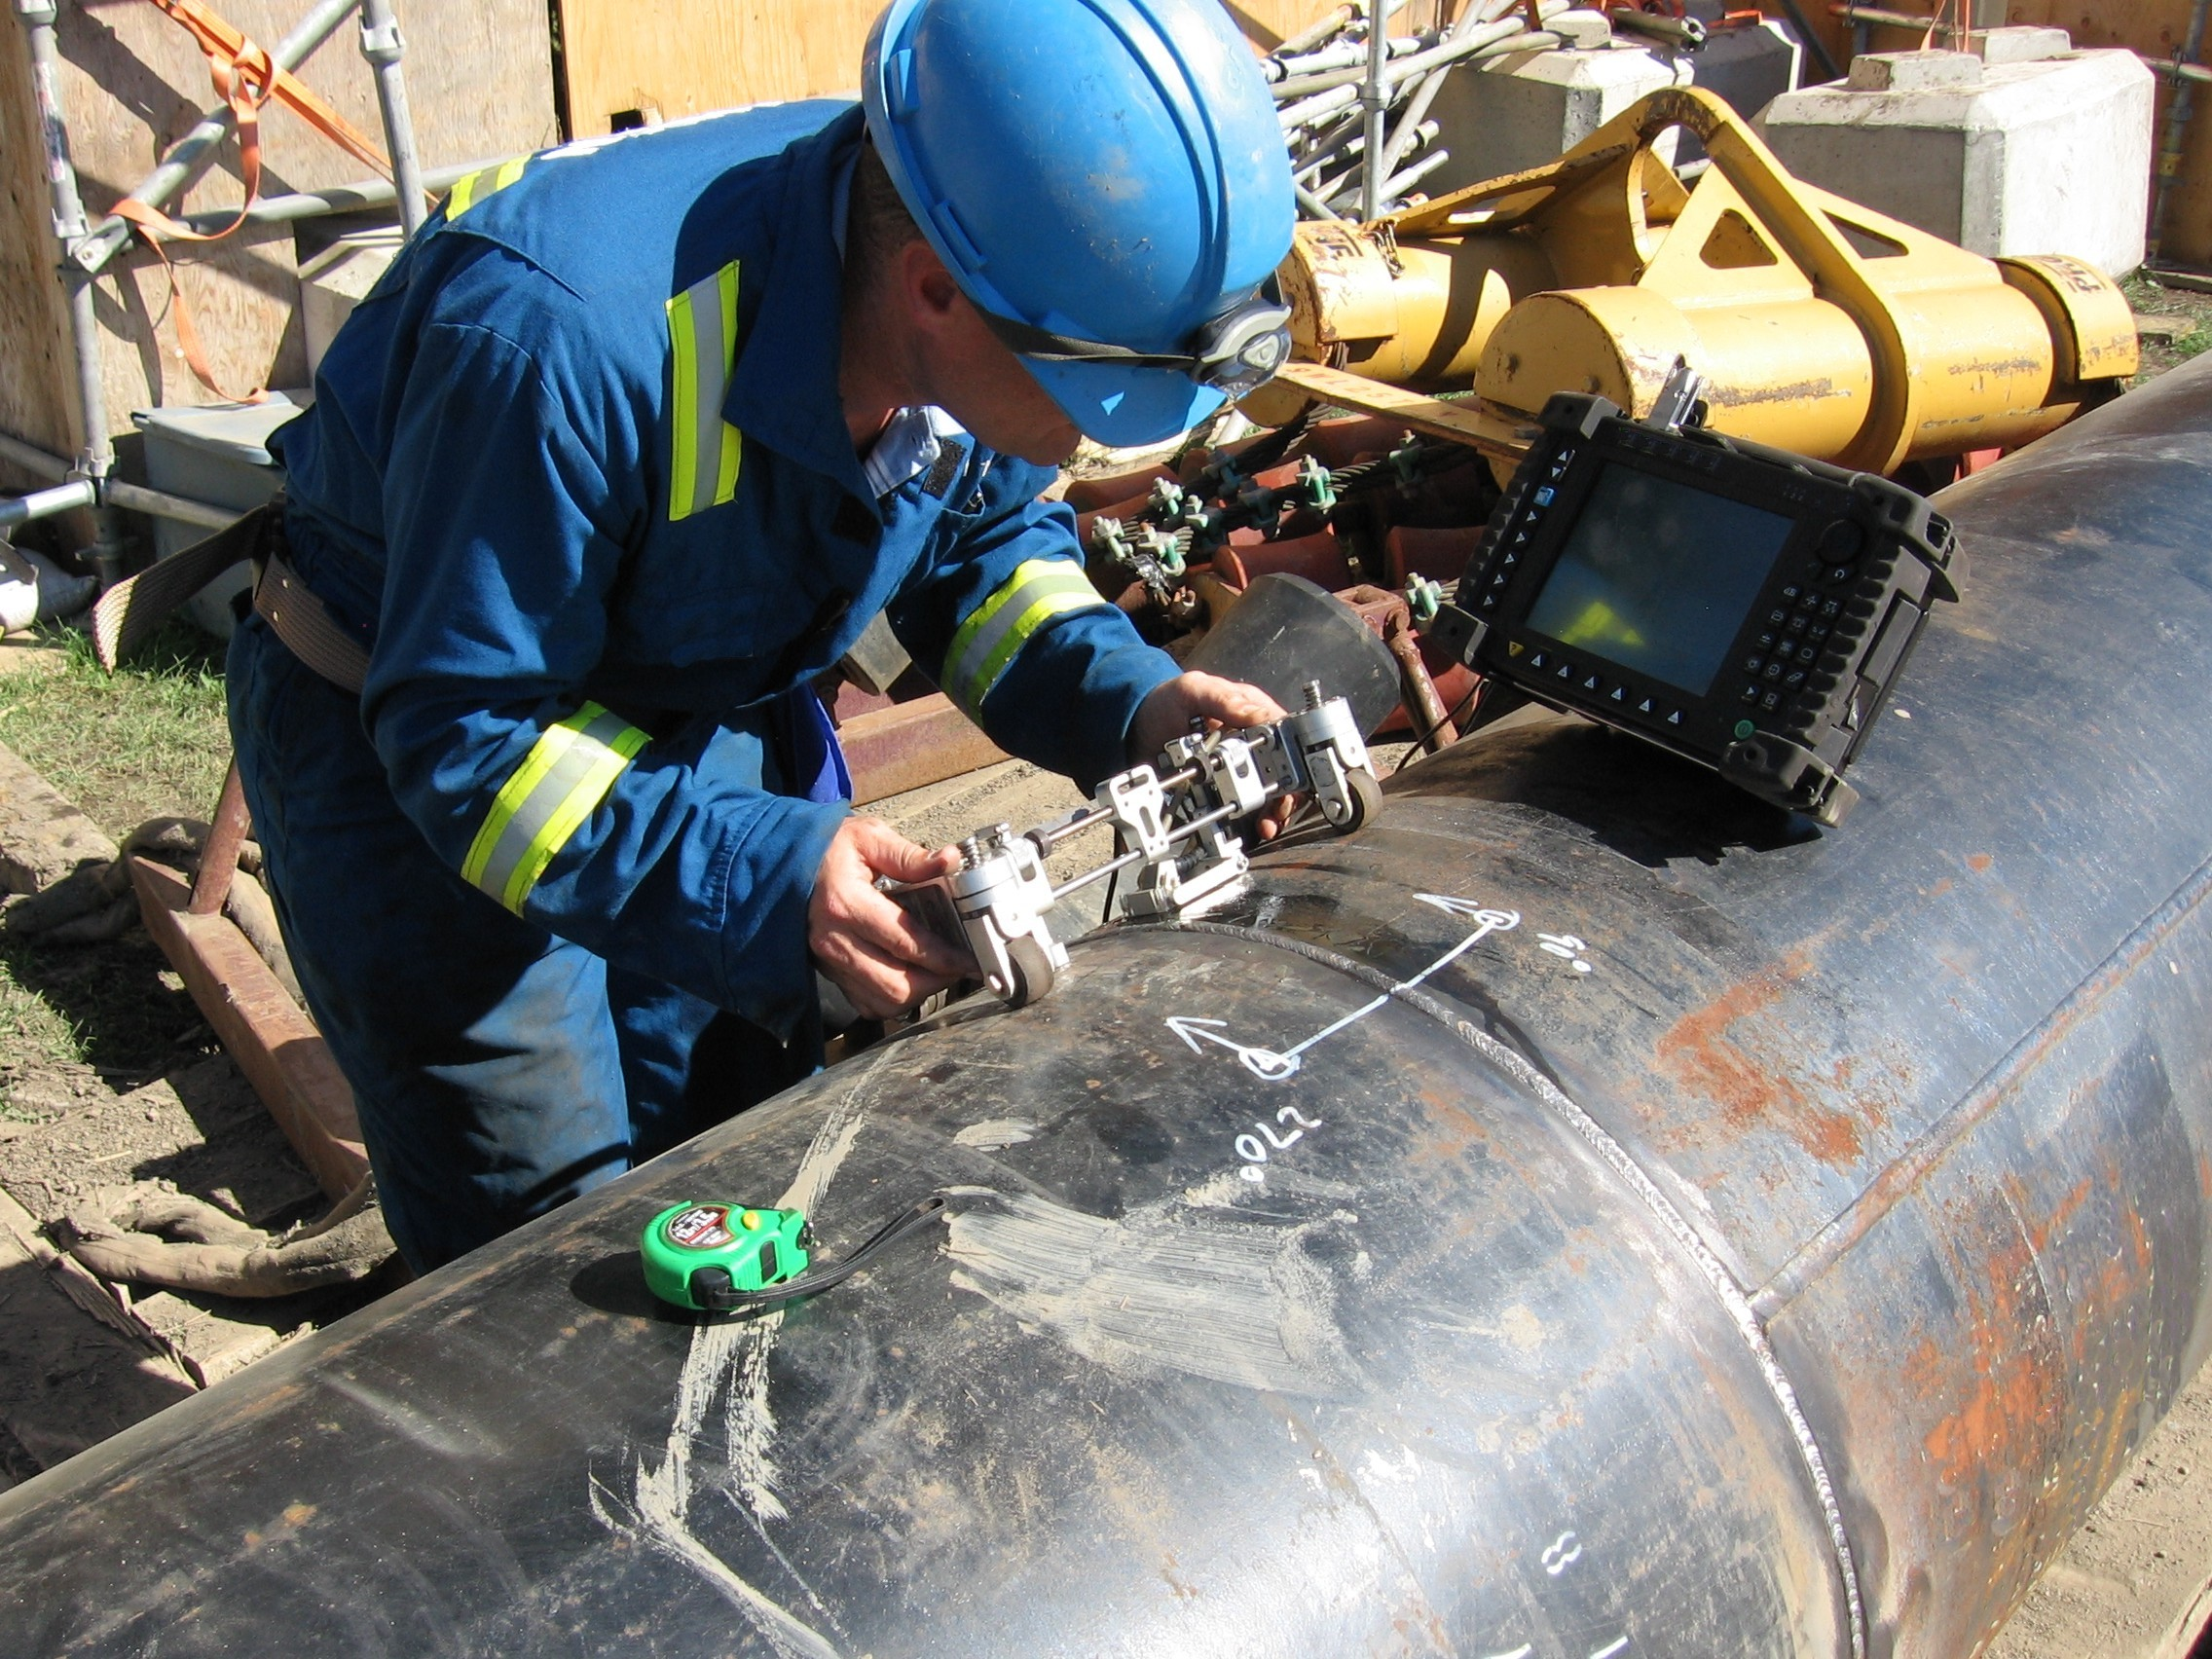
\includegraphics[height=3cm]{img/us_test.jpg}\\
				{\tiny{\raggedright \itshape Picture from Davidmack}\\ \centering \scriptsize{Pipeline test}}
			\end{figure}		
			\column{0.5\textwidth}
			\begin{figure}
				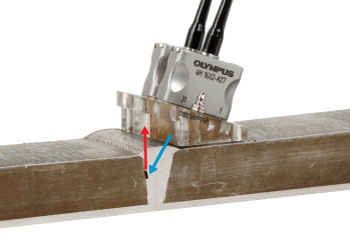
\includegraphics[height=3cm]{img/olympus.jpg}\\
				 {\tiny{\itshape Picture from Olympus}\\ \centering			\scriptsize{Echo mode testing}}
			\end{figure}
		\end{columns}	
		\vspace{0.6cm}	

	%\begin{columns}
			%\column{.5\textwidth}
			Non destructive testing for weld in :\\
			\begin{itemize}
				\item nuclear reactors (cooling system)
				\item oil and gaz pipelines 
			\end{itemize}
			%\column{.05\textwidth}
			%\ding{222}
			%\column{.45\textwidth}
			%\centering
			\vspace{0.6cm}
 			\indent \ding{222} porosity, cracks, lack of fusion, corrosion, inclusions,. . .
	%\end{columns}
\end{frame}

\begin{frame}{\insertsectionhead}
\vspace{-1cm}
\hspace{1cm}
	\begin{columns}[c]
			\column{.5\textwidth}<1->
			\centering
			\begin{figure}
				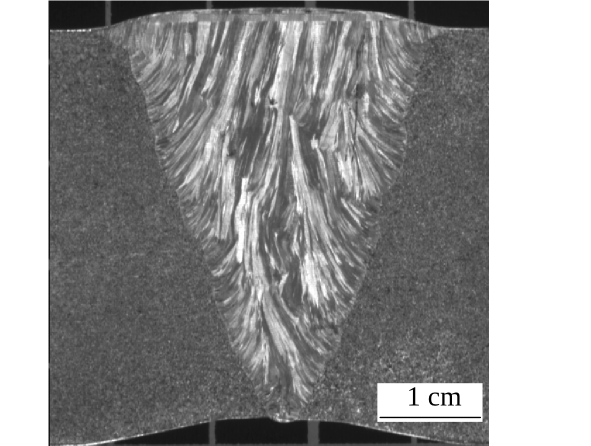
\includegraphics[height=2.7cm]{./img/soudure1.png}\\
				{\tiny{ \itshape Picture from Chassignole, 2010 (PhD thesis)} \\ \centering \scriptsize Macrography of a weld }
			\end{figure}
			\column{.001\textwidth}<2->
			\hspace{-3cm}
			\vspace{2cm}
			\begin{tikzpicture}
					\draw[<-, thick,shorten <=2pt,shorten >=2pt,red] (-1.5,3)--(0.5,4);
			\end{tikzpicture}
			\column{.9\textwidth}<2->
			%\vfill
			\hspace{-1cm}
			\textcolor{red}{Strong unknown anisotropy}\\
			$\hookrightarrow$ distorsion and splitting of the beam\\[0.2cm]
			\hspace{-0.5cm}
			\hspace{2cm} 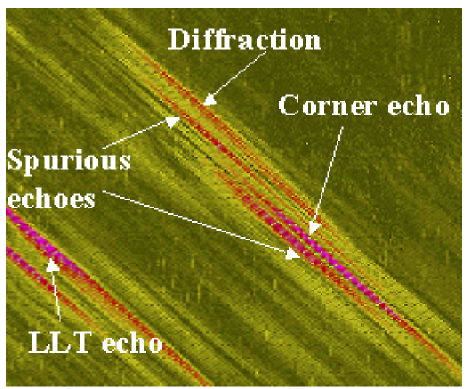
\includegraphics[height=2cm]{img/chassignole_echos.png}\\
			\hspace{1cm} {\tiny{ \itshape Picture from Chassignole, 2010 (PhD thesis)} \\ \centering \scriptsize Comparison of ray based model and experiment result } 
				
	\end{columns}
	\vspace{0.3cm}
	\begin{columns}[c]
			\column{.5\textwidth}<1->
			%\begin{block}{}
				\begin{itemize}
					\item[$\bullet$] delay and sum methods
					\item[$\bullet$] decomposition of covariance matrix (DORT)
				\end{itemize}
			%\end{block}
			\column{.05\textwidth}<2->
			\ding{222}
			\column{.5\textwidth}<2->
			%\begin{block}{}
				\begin{itemize}
					\item[\ding{55}] need to know $c$ a priori\\
					\item[\ding{55}] strong artefacts
				\end{itemize}
			%\end{block}
			
	\end{columns}
	\begin{columns}[c]
		\column{.5\textwidth}<3->
			\begin{itemize}
				\item[$\bullet$] solving NL optimization problem
			\end{itemize}
		\column{.05\textwidth}<3->
			\ding{222}
		\column{.5\textwidth}<3->
			\begin{itemize}
			\item contour reconstruction :\\\hspace{-0.5cm}\small{\emph{Dominguez et al.}, \emph{Rodriguez et al.}}\\[0.1cm]
			\item[\ding{51}] \normalsize{$C_{ij}$ reconstruction : FWI}
		\end{itemize}		
	\end{columns}
\end{frame} 

\section{What is specific to weld imaging ?}
\begin{frame}{\insertsectionhead}
	\begin{itemize}
		\item <1-> 2 free surfaces : more information $\leftrightarrow$ non-linear inversion
		\item <2-> surface acquisition only 
		\item <3-> anisotropy $\rightarrow$ multi-parameter inversion \\\hspace{2.3cm}($C_{ij}\times$6 : weld + defects)
		%\item <4-> defects $\rightarrow$ multi-scale inversion ($C_{ij}^{d}\times$6)
	\end{itemize}
	\vfill
	\begin{figure}[!h]
		\centering
		\includegraphics<1-1>[scale=1]{img/soud1.pdf}
		\includegraphics<2-2>[scale=1]{img/soud2.pdf}
		%\includegraphics<3-3>[scale=1]{img/soud3.pdf}
		\includegraphics<3-3>[scale=1]{img/soud4_bis.pdf}
	\end{figure}

\end{frame}



\section{Resolution analysis}

\begin{frame}{\insertsectionhead}
	\only<1-3>{
		\begin{equation*}
			\frac{\partial C}{\partial m_{i}}= \textcolor{DeepSkyBlue4}{\underbrace{\textcolor{black}{\tr{\tilde{\bm{d}}_{cal}}}}_{\substack{\text{incident}\\ \text{wavefield}}}}
			 \tr{\left( \frac{\partial\bm{A}}{\partial m_{i}} \right)} 
			 \textcolor{DeepSkyBlue4}{\underbrace{\textcolor{black}{\bm{\lambda}}}_{\substack{\text{back-propagated} \\ \text{residual wavefields}}}}
		\end{equation*}
	}
%	\only<4->{
%		\vspace{-0.06cm}\begin{equation*}
%			\frac{\partial C}{\partial m_{i}}= \textcolor{DeepSkyBlue4}{\underbrace{\textcolor{black}{\tr{\tilde{\bm{d}}_{cal}}}}_{\substack{\text{champ incident}}}}
%			 \text{\fcolorbox{DeepSkyBlue4}{white!0}{$\tr{\left( \frac{\partial\bm{A}}{\partial m_{i}} \right)}$ }}
%			 \textcolor{DeepSkyBlue4}{\underbrace{\textcolor{black}{\bm{\lambda}}}_{\substack{\text{résidus rétropopagés}}}}
%		\end{equation*}		
%	\begin{picture}(0,0)(0,0)\put(155,-105){
%		\begin{tikzpicture}	
%					\node (A) at (6,0) {};
%					\node (ray) at ($(A)+(0,-4)$) {};
%					\draw[->, thick,shorten <=2pt,shorten >=2pt,DeepSkyBlue4] (A) -- (ray);		
%		\end{tikzpicture}
%	}\end{picture}
%	}
	\begin{equation*}
		~~~~~~~~\sim~ \Re\left( e^{j k_{0} \bm{s.x}} \right)~~~~~~~~~\sim~ \Re\left( e^{j k_{0} \bm{r.x}} \right)
	\end{equation*}
		
	\onslide<2->{
		\begin{itemize}
			\item Gradient resolution : \vspace{-0.2cm}
			\begin{align}
				k=|\bm{s}+\bm{r}|=&\frac{\omega}{c}2\cos\left( \frac{\theta}{2} \right)~~~~~~~~\\
			\end{align}	\vspace{-1cm}		
	}
		\only<1-3>{
			\begin{columns}
				\column{0.4\textwidth}<1-3>
				\begin{figure}
					\centering
					\vfill
					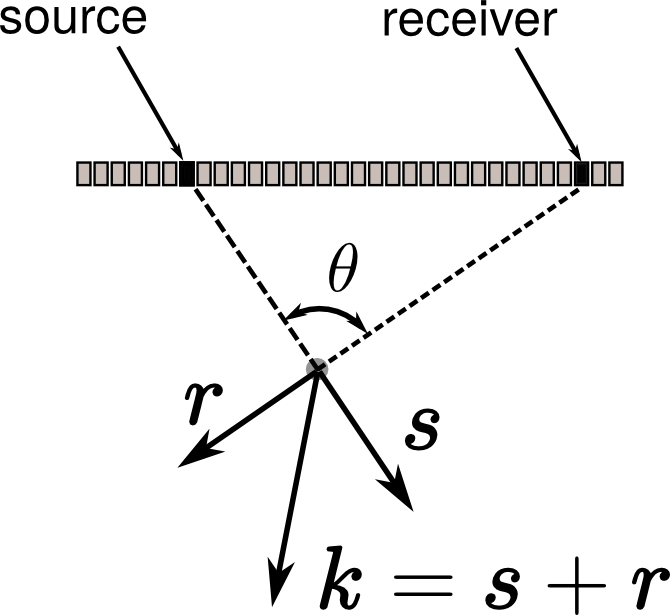
\includegraphics[height=2.5cm]{img/reso.png}	
				\end{figure}
				\column{0.55\textwidth}<3-3>
				\begin{figure}
					\centering
					\vspace{0.4cm} 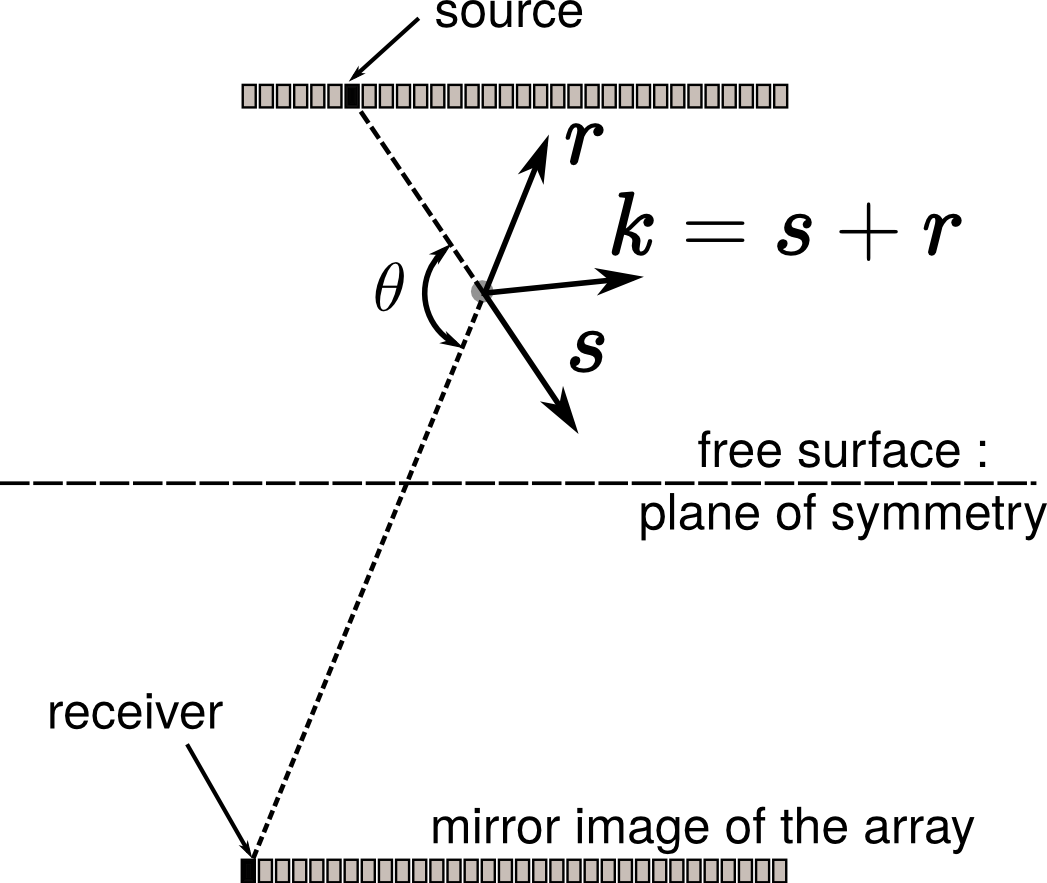
\includegraphics[height=3.7cm]{img/reso_surf_libre.png}
				\end{figure}		
			\end{columns}
		}
	
%
%	\only<4->{		
%		\vspace{0.7cm}\item Radiation patterns :\\[0.2cm] 
%		\begin{figure}
%			\hspace{-1cm}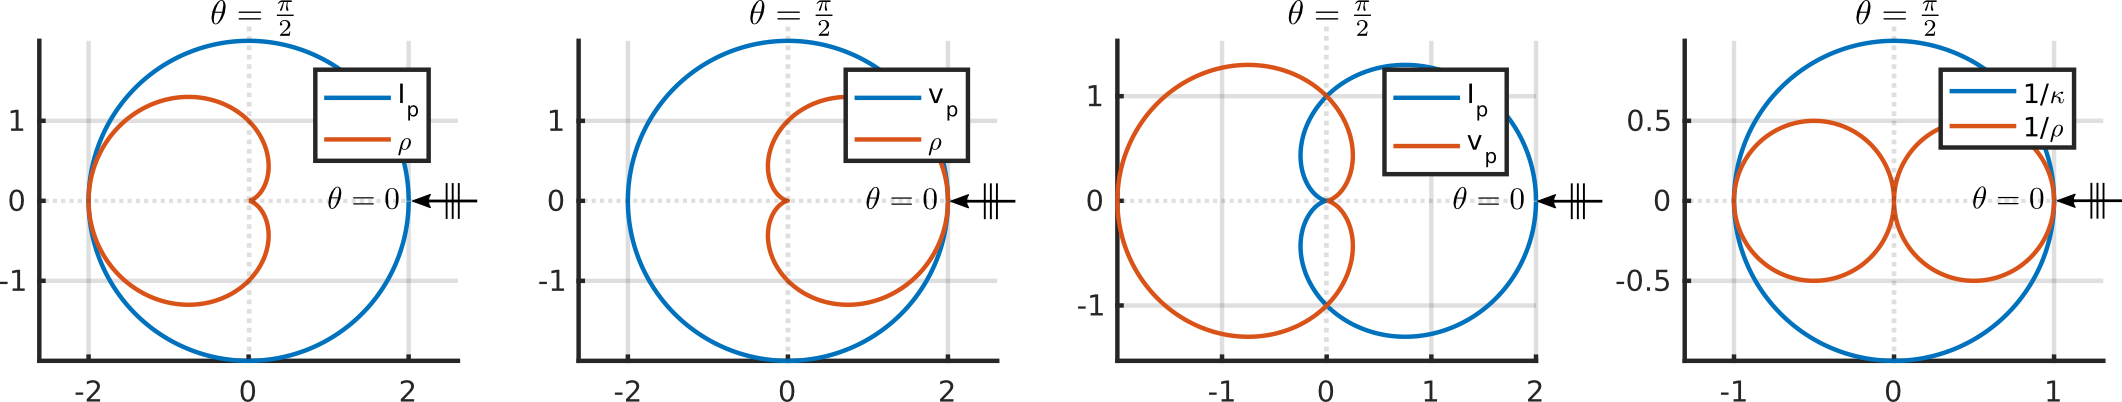
\includegraphics[height=2cm]{img/rayonnement.png}
%		\end{figure}		
%	}

	\end{itemize}
	\vspace{1cm}
\end{frame}




\begin{frame}{\insertsectionhead~-- Local 2DFT}
	\begin{figure}
		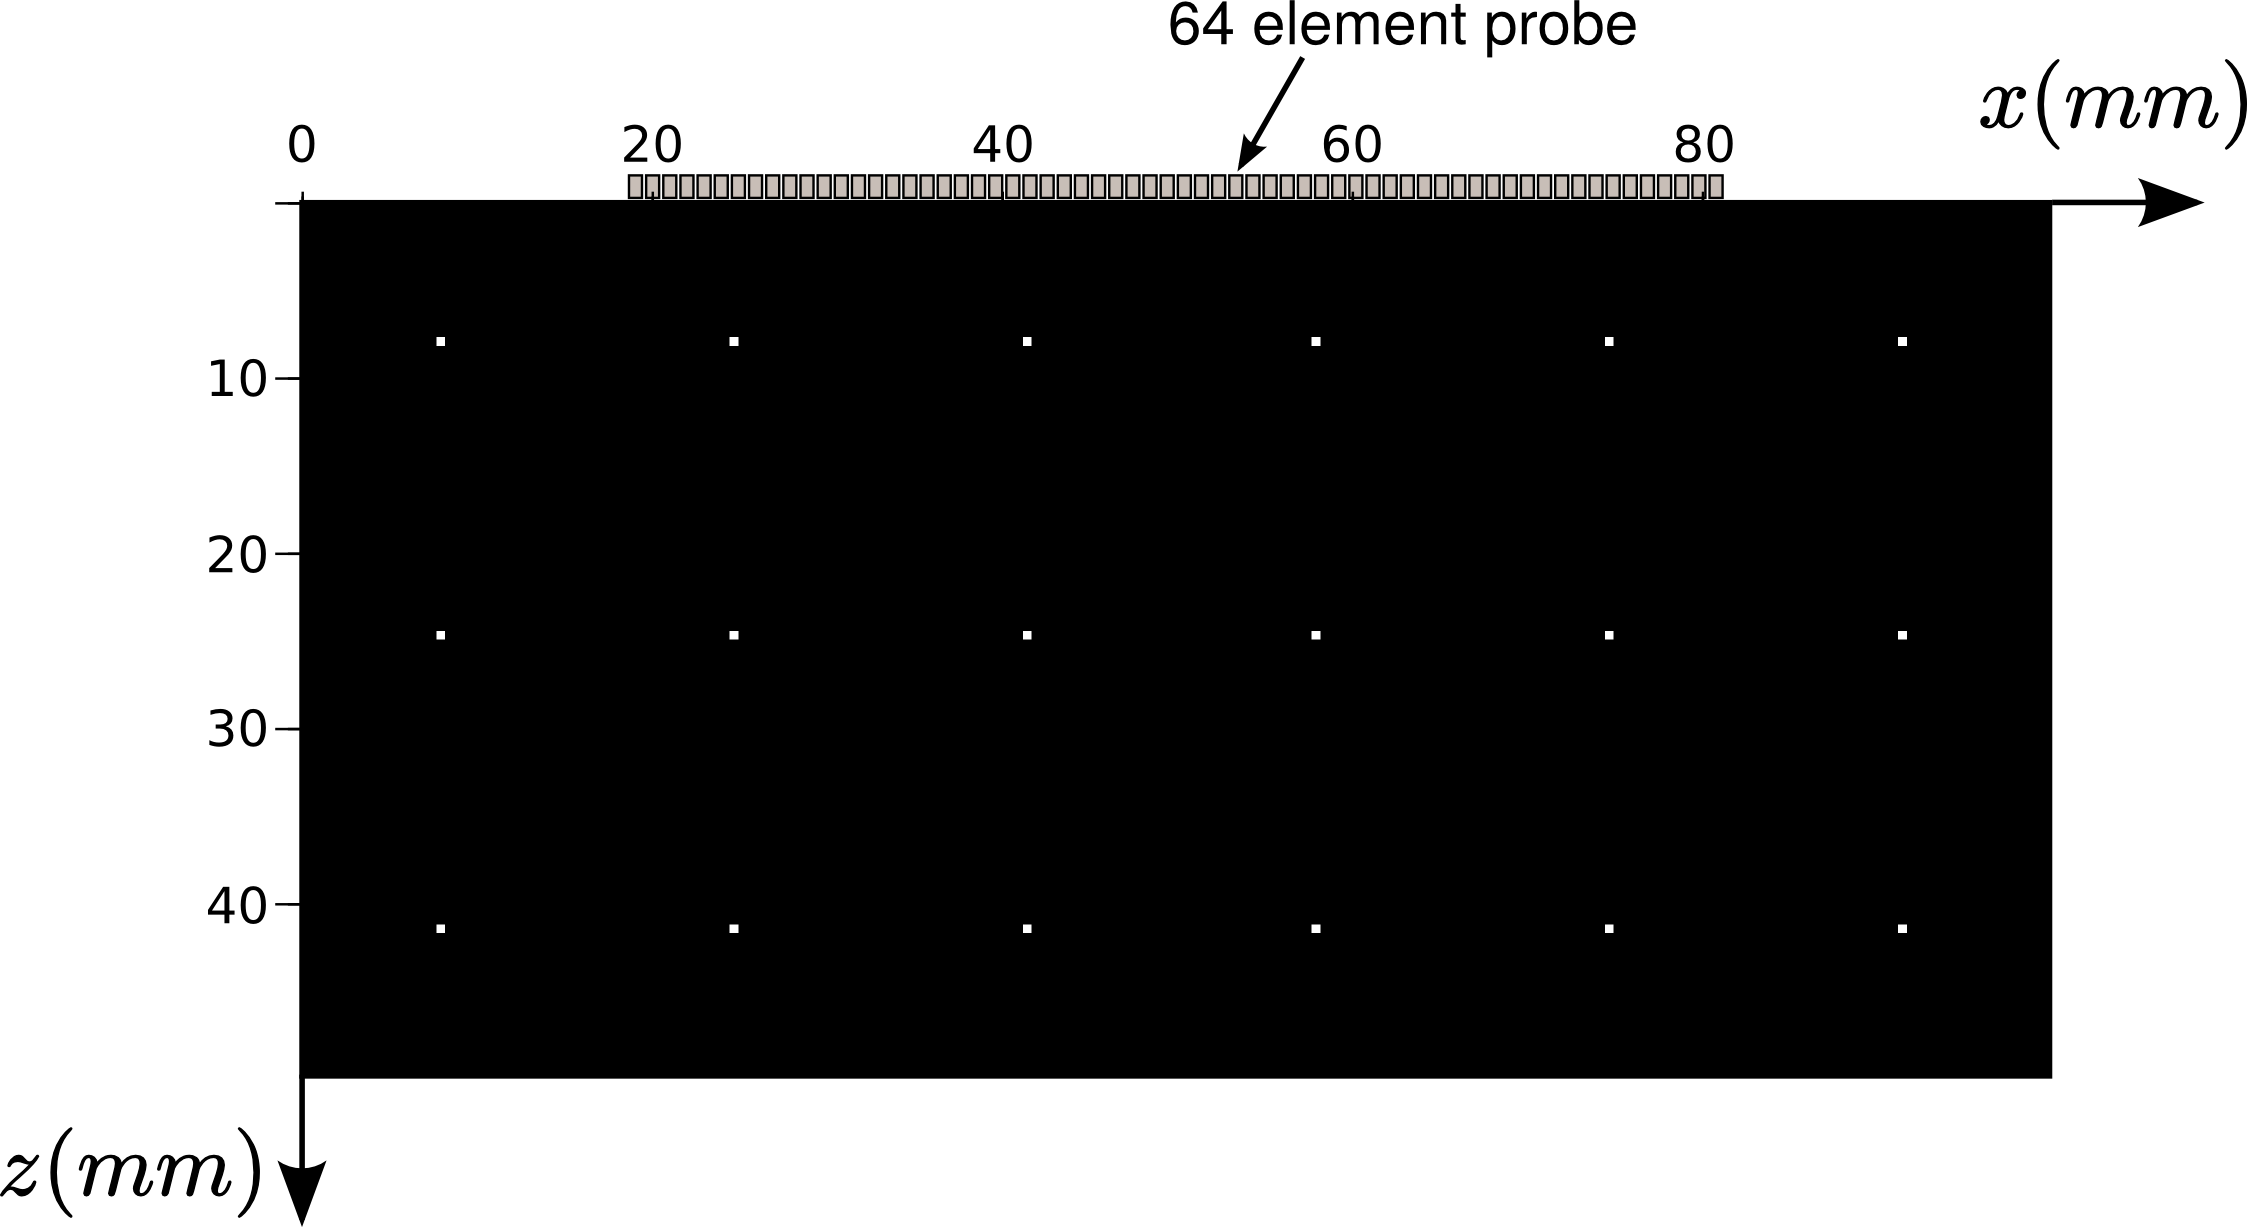
\includegraphics[height=2.5cm]{img/vp_scat.png}\\
		\vspace{-0.3cm} \small{Velocity model}
	\end{figure}
	\vspace{-0.6cm} 
	\begin{columns}
		\column{0.5\textwidth}
		\begin{figure}
			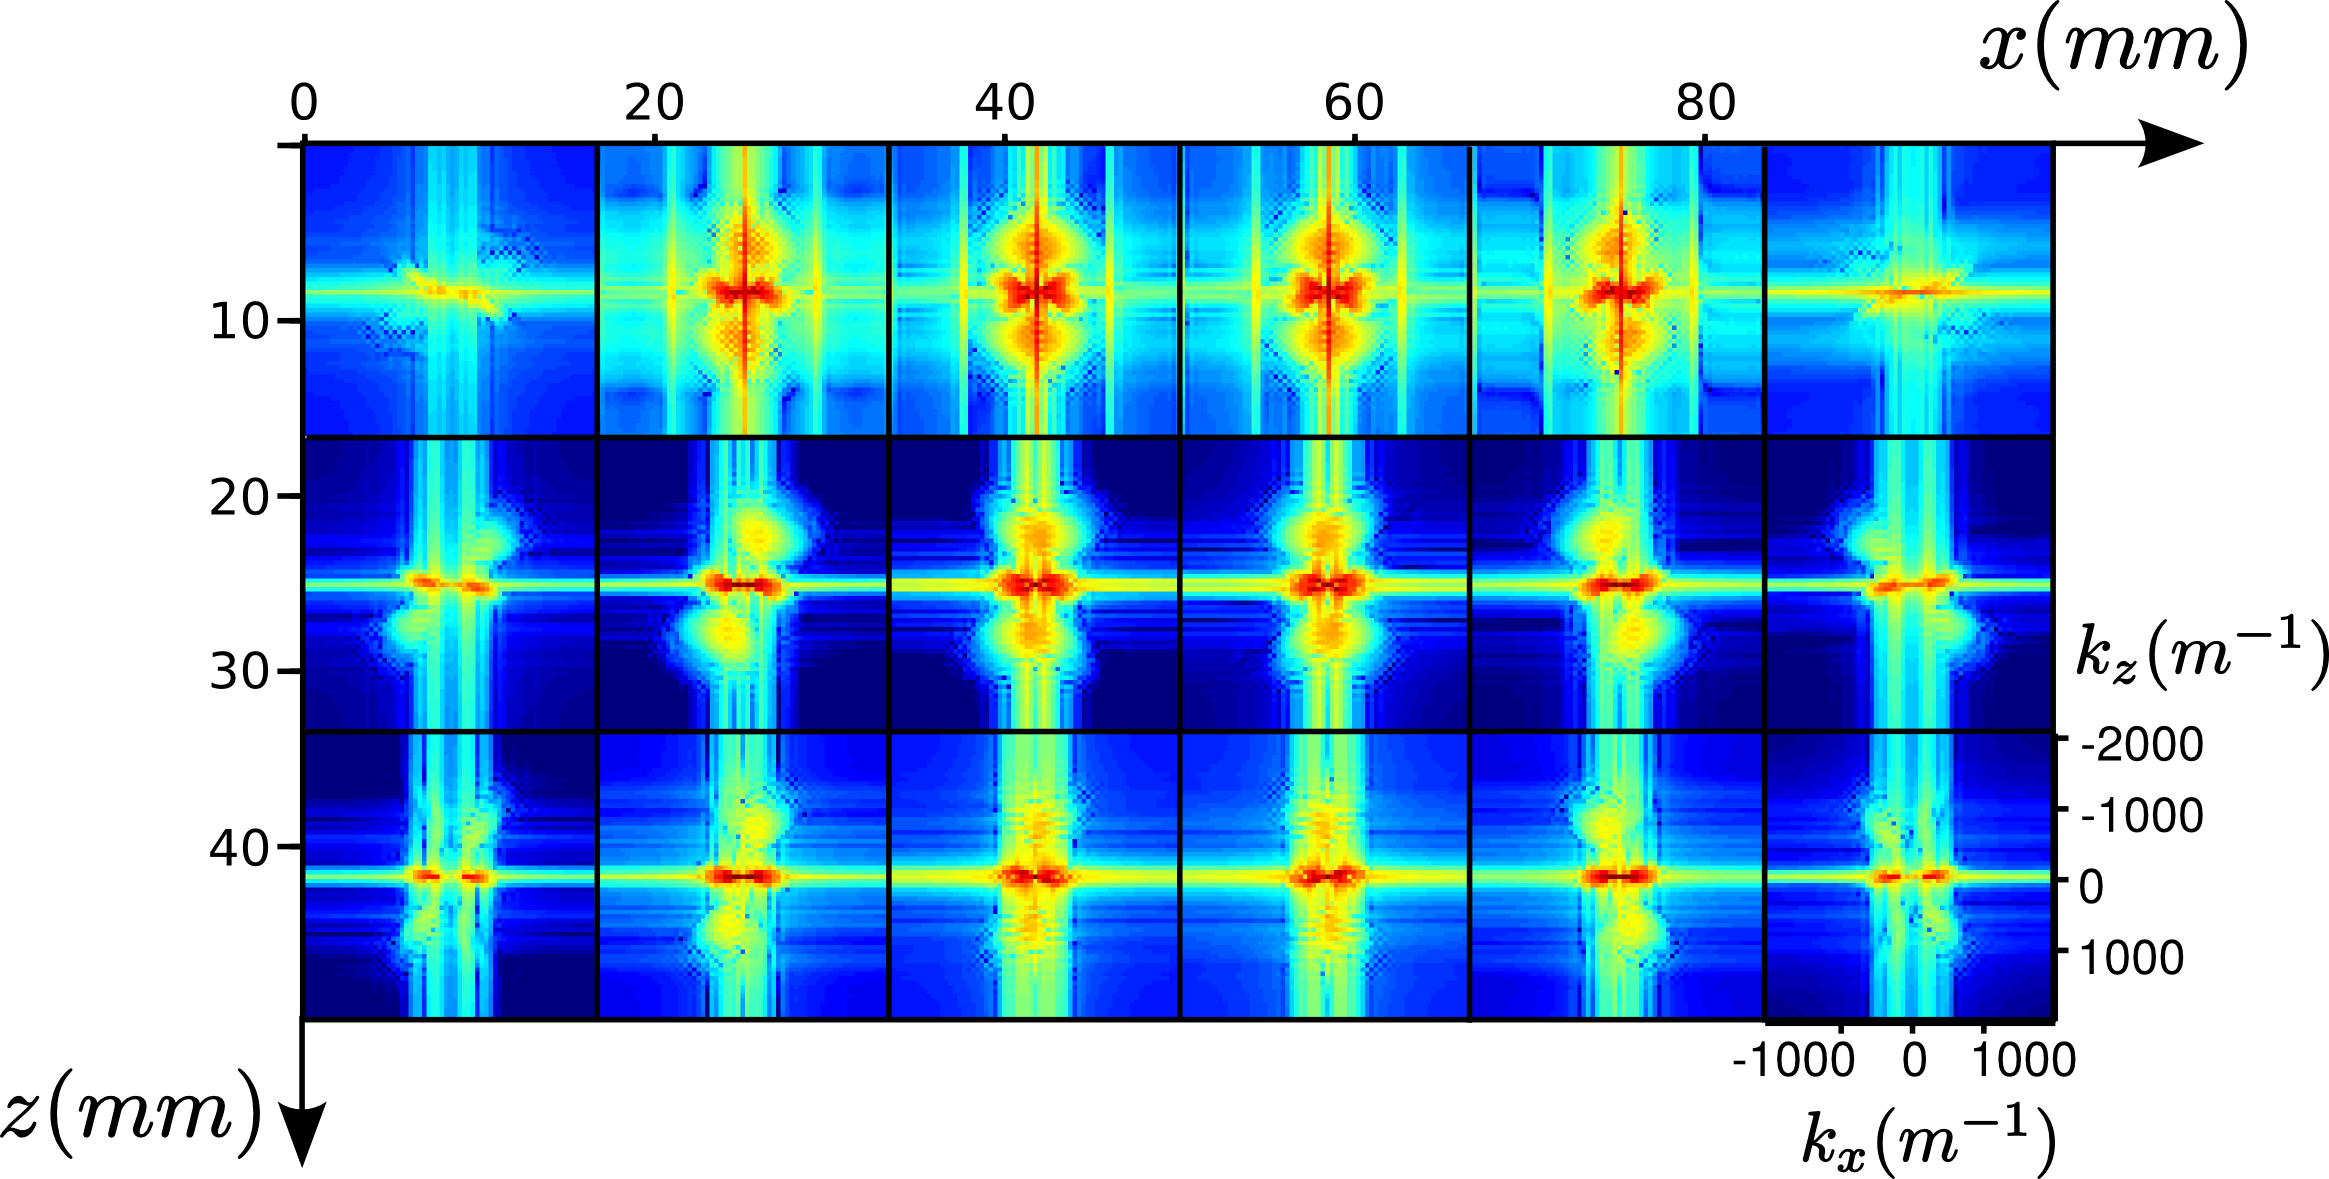
\includegraphics[height=3cm]{img/1400pt.png}\\
			\small{For 1 reflection}\\[0.3cm]
			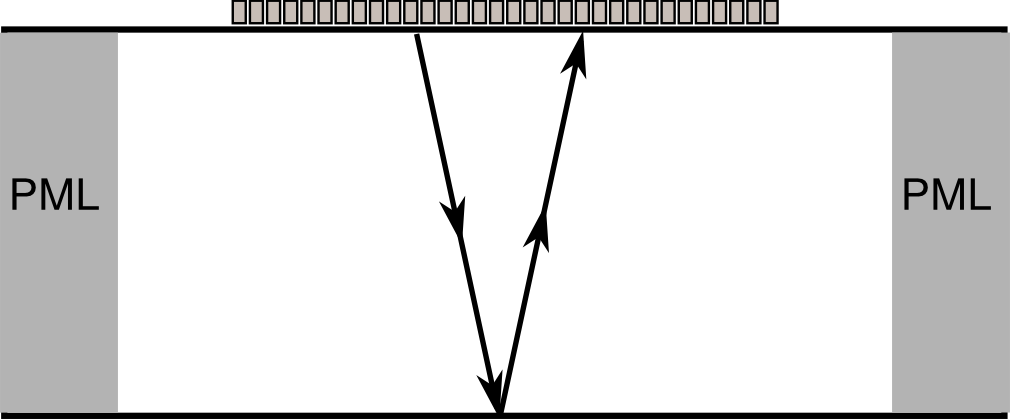
\includegraphics[height=1cm]{img/1ref.png}
		\end{figure}
		\column{0.5\textwidth}
		\begin{figure}
			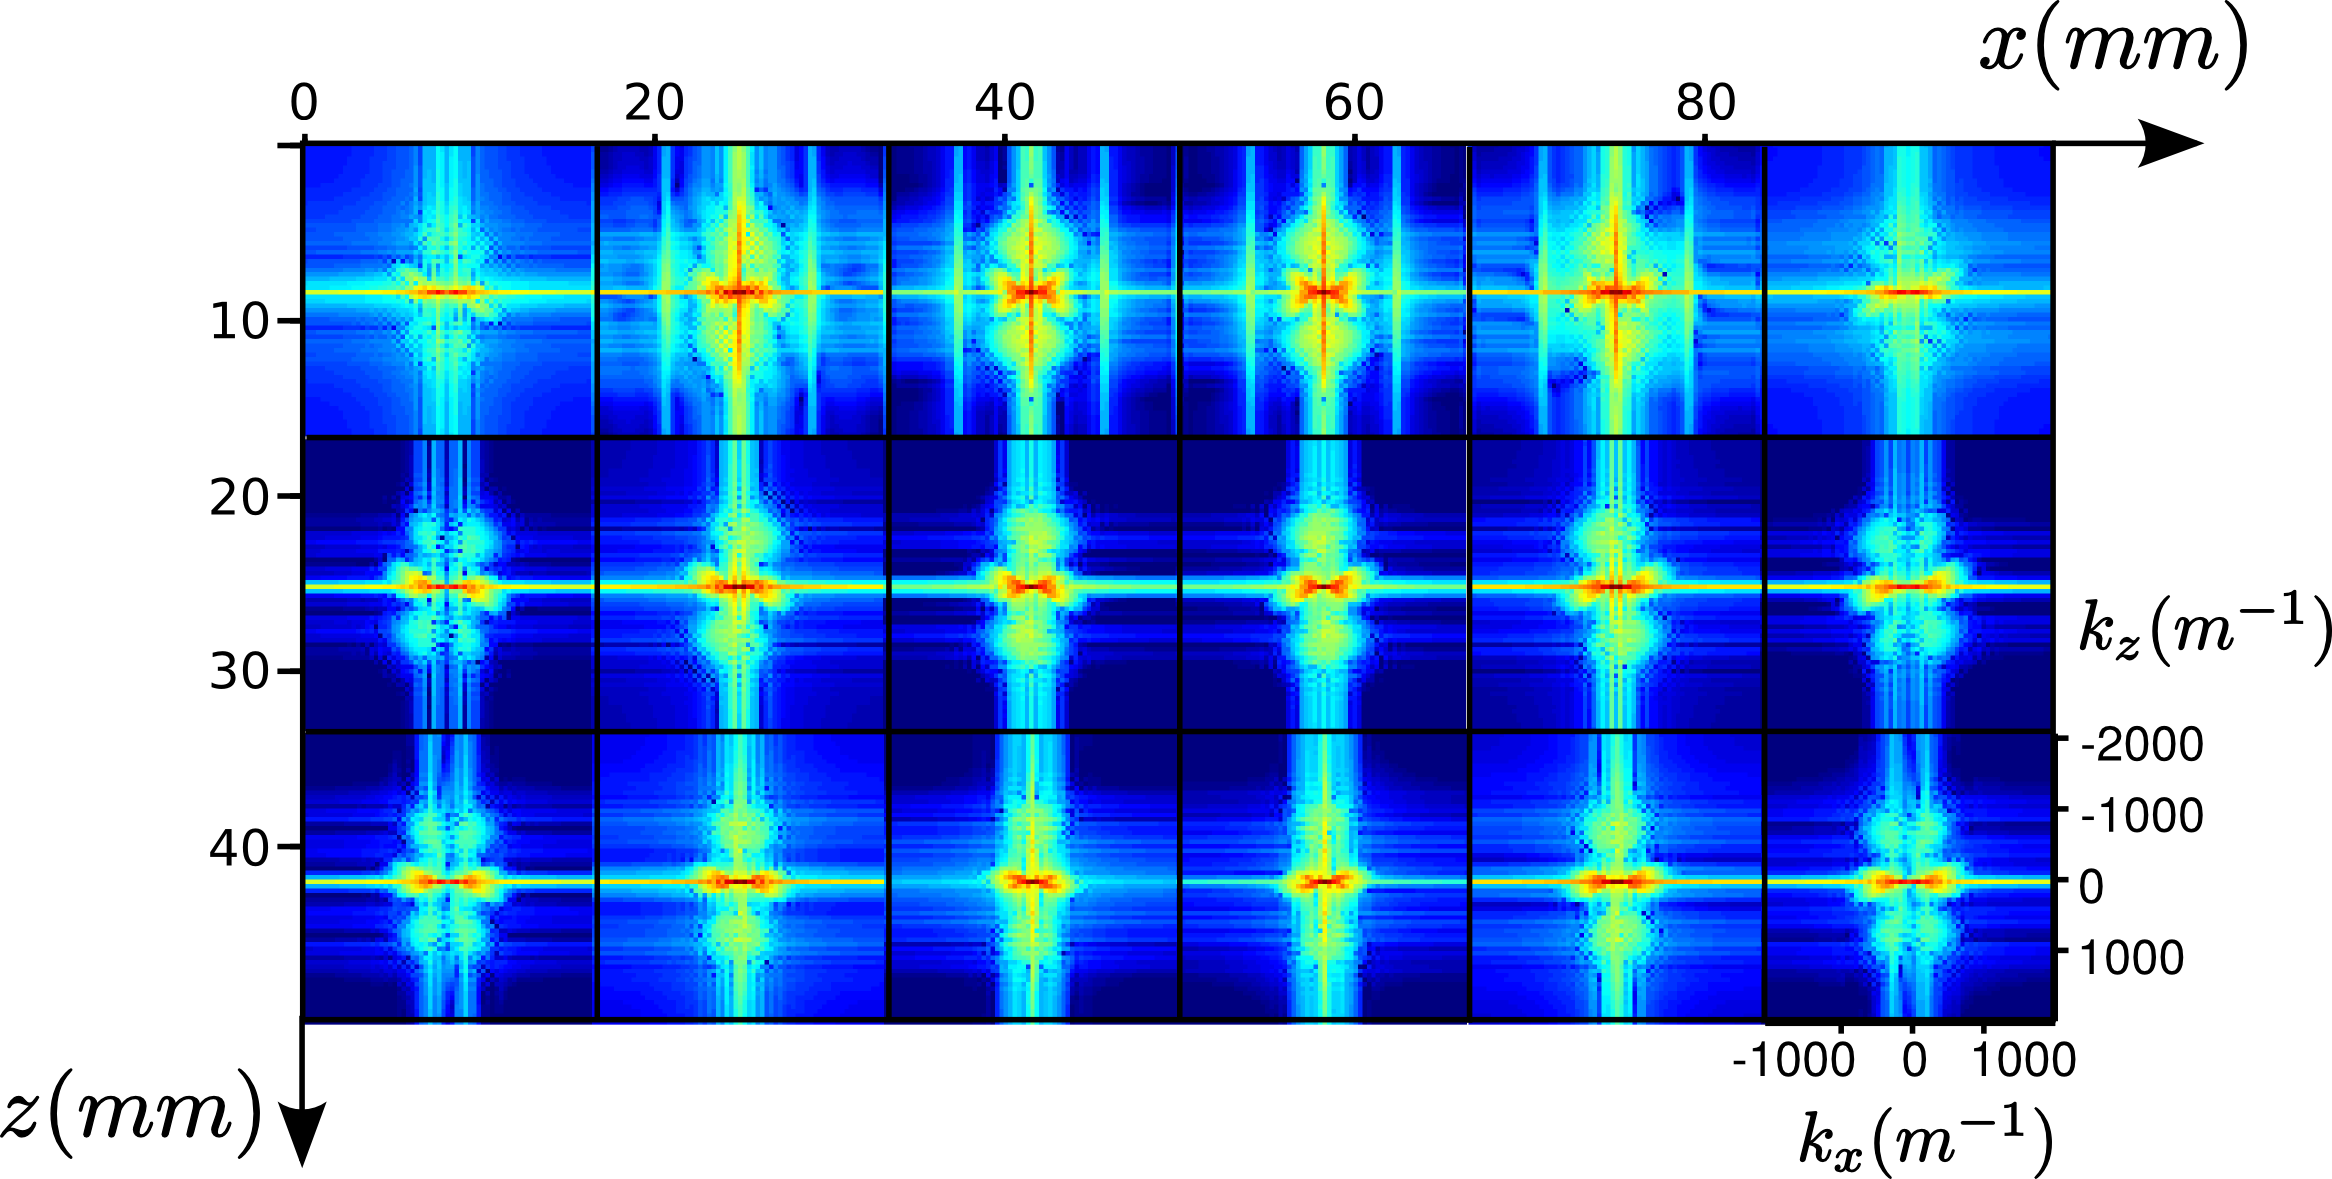
\includegraphics[height=3cm]{img/4200pt.png}\\
			\small{For 5 reflections}\\[0.3cm]
			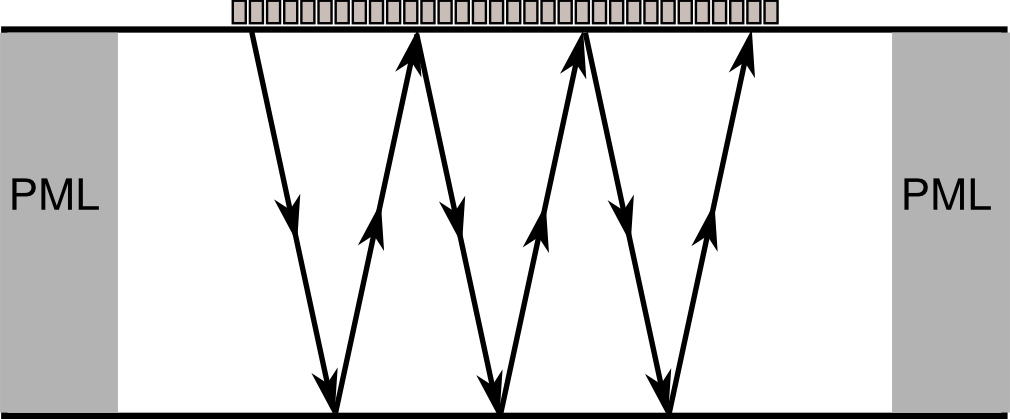
\includegraphics[height=1cm]{img/6ref.png}
		\end{figure}
	\end{columns}

\end{frame}

%\begin{frame}{Synthetic case}
%	
%	\begin{columns}
%		\column{0.5\textwidth}
%		plop
%	\end{columns}	
%	
%	ideal acquisiation
%	vp true, rho true
%	freq + nb of prop wavelength
%
%\end{frame}


\section{Isotropic Synthetic case}
\subsection*{}
\begin{frame}{\insertsectionhead}
	\begin{itemize}
		\item<1-> 2D, isotropic, acoustic (\emph{TOYxDAC\_TIME\_V1.5})
		\item<1-> Parametrisation : $v_{p}$ and $\rho$
		\item Recording time : 1 reflexion
		\item<2-> Excitation frequency : 2 MHz
	\end{itemize}
	\only<1-1>{
	\begin{columns}
		\column{0.5\textwidth}
		\begin{figure}
			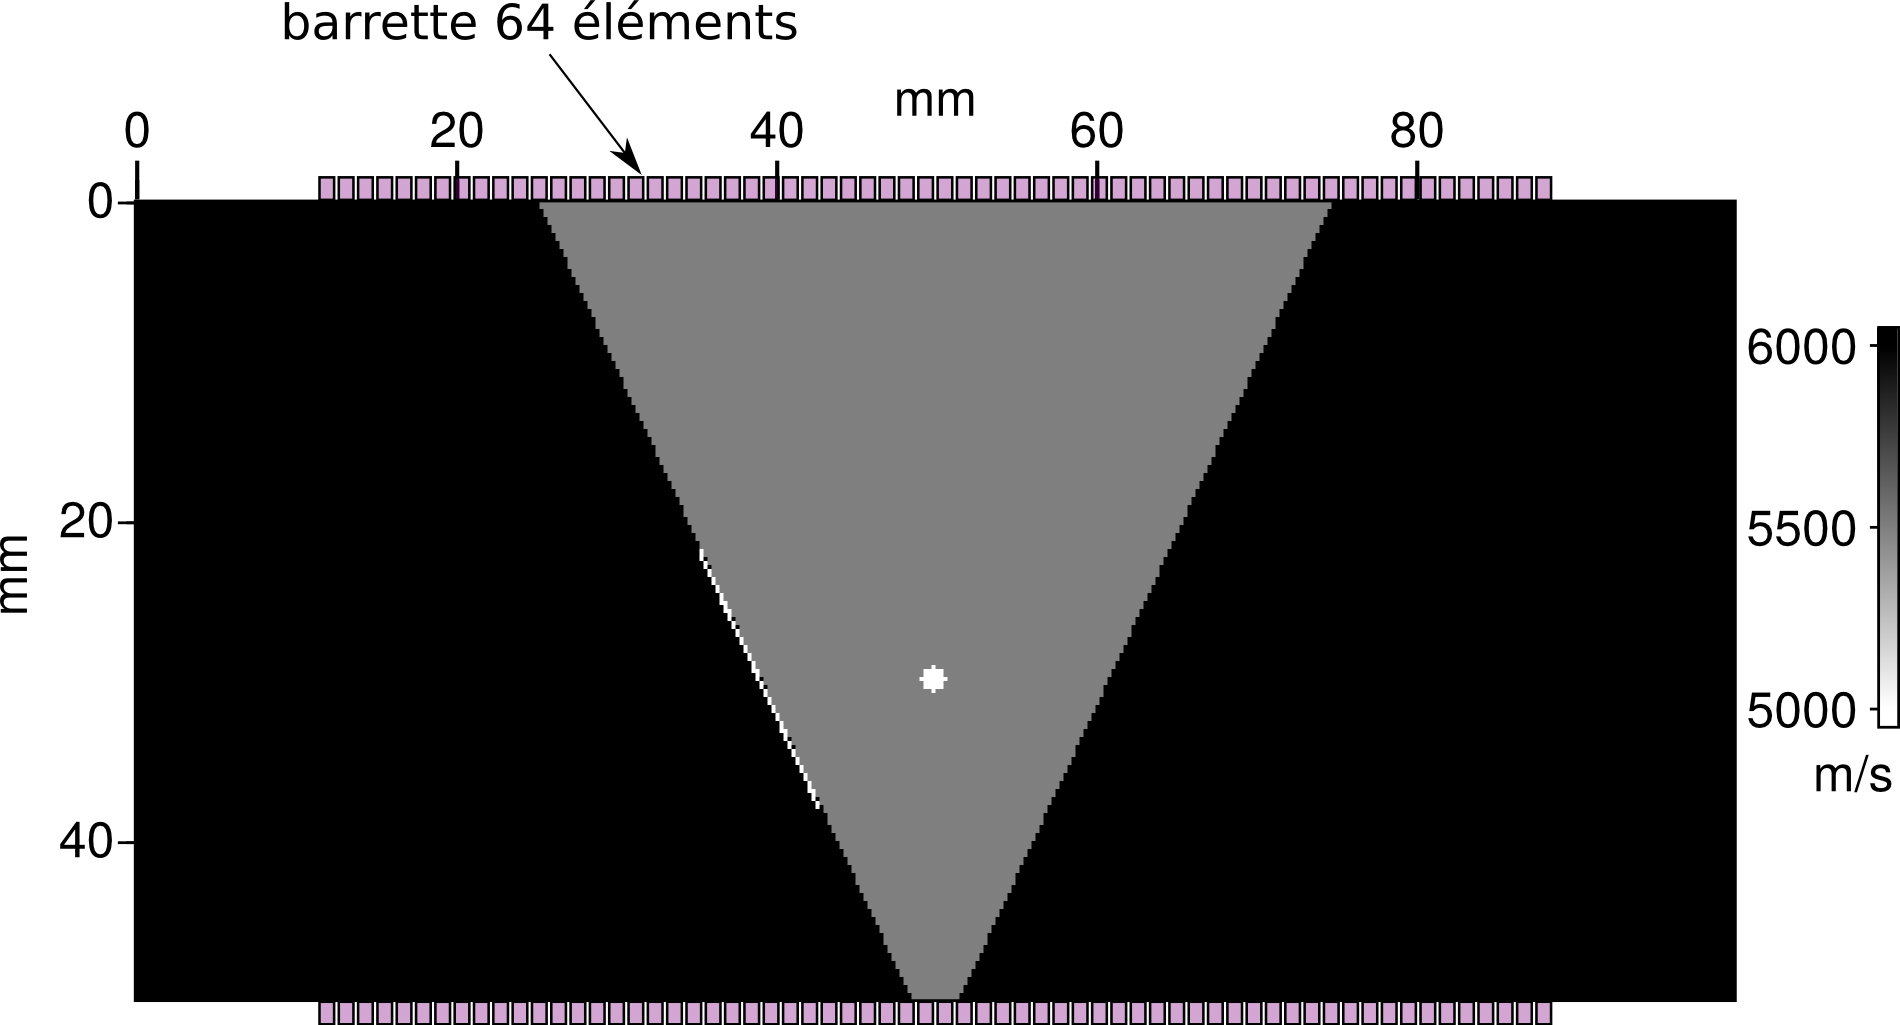
\includegraphics[width=\textwidth]{img/vp_true.png}\\
			{\small True velocity}
		\end{figure}
		\column{0.5\textwidth}
		\begin{figure}
			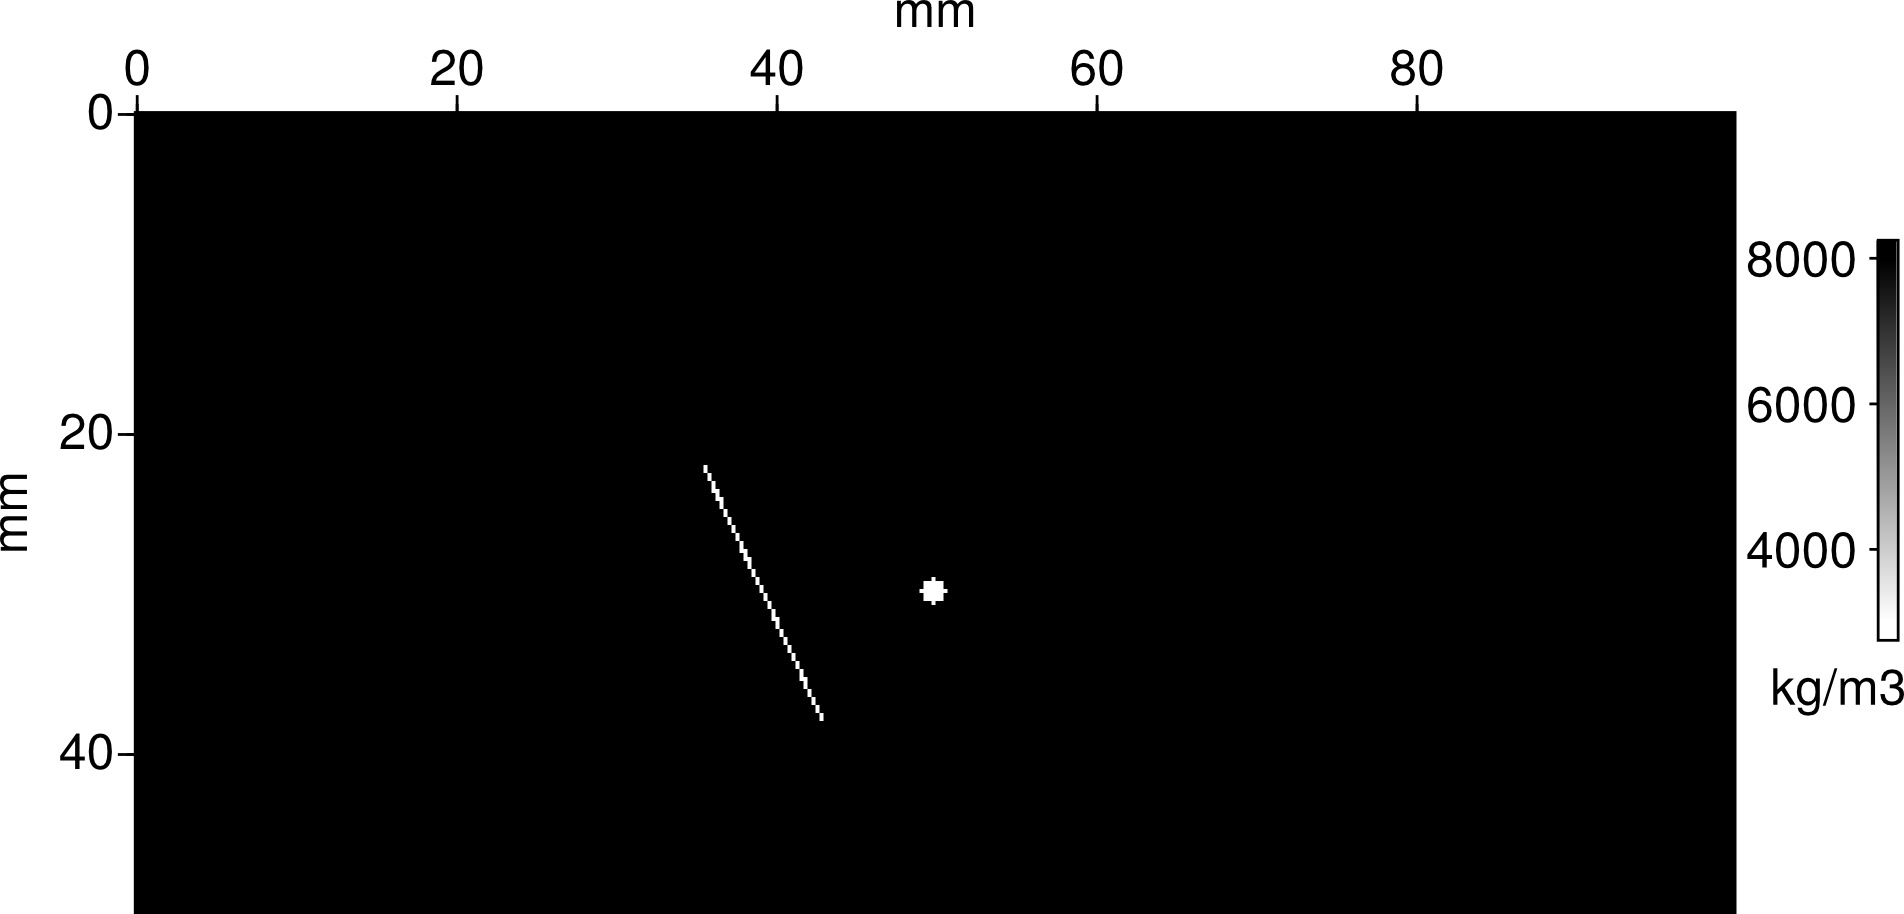
\includegraphics[width=\textwidth]{img/rho_true.png}\\
			{\small True density}
		\end{figure}
	\end{columns}
	}
	
	\only<2->{
	\begin{columns}
		\column{0.5\textwidth}
		\begin{figure}
			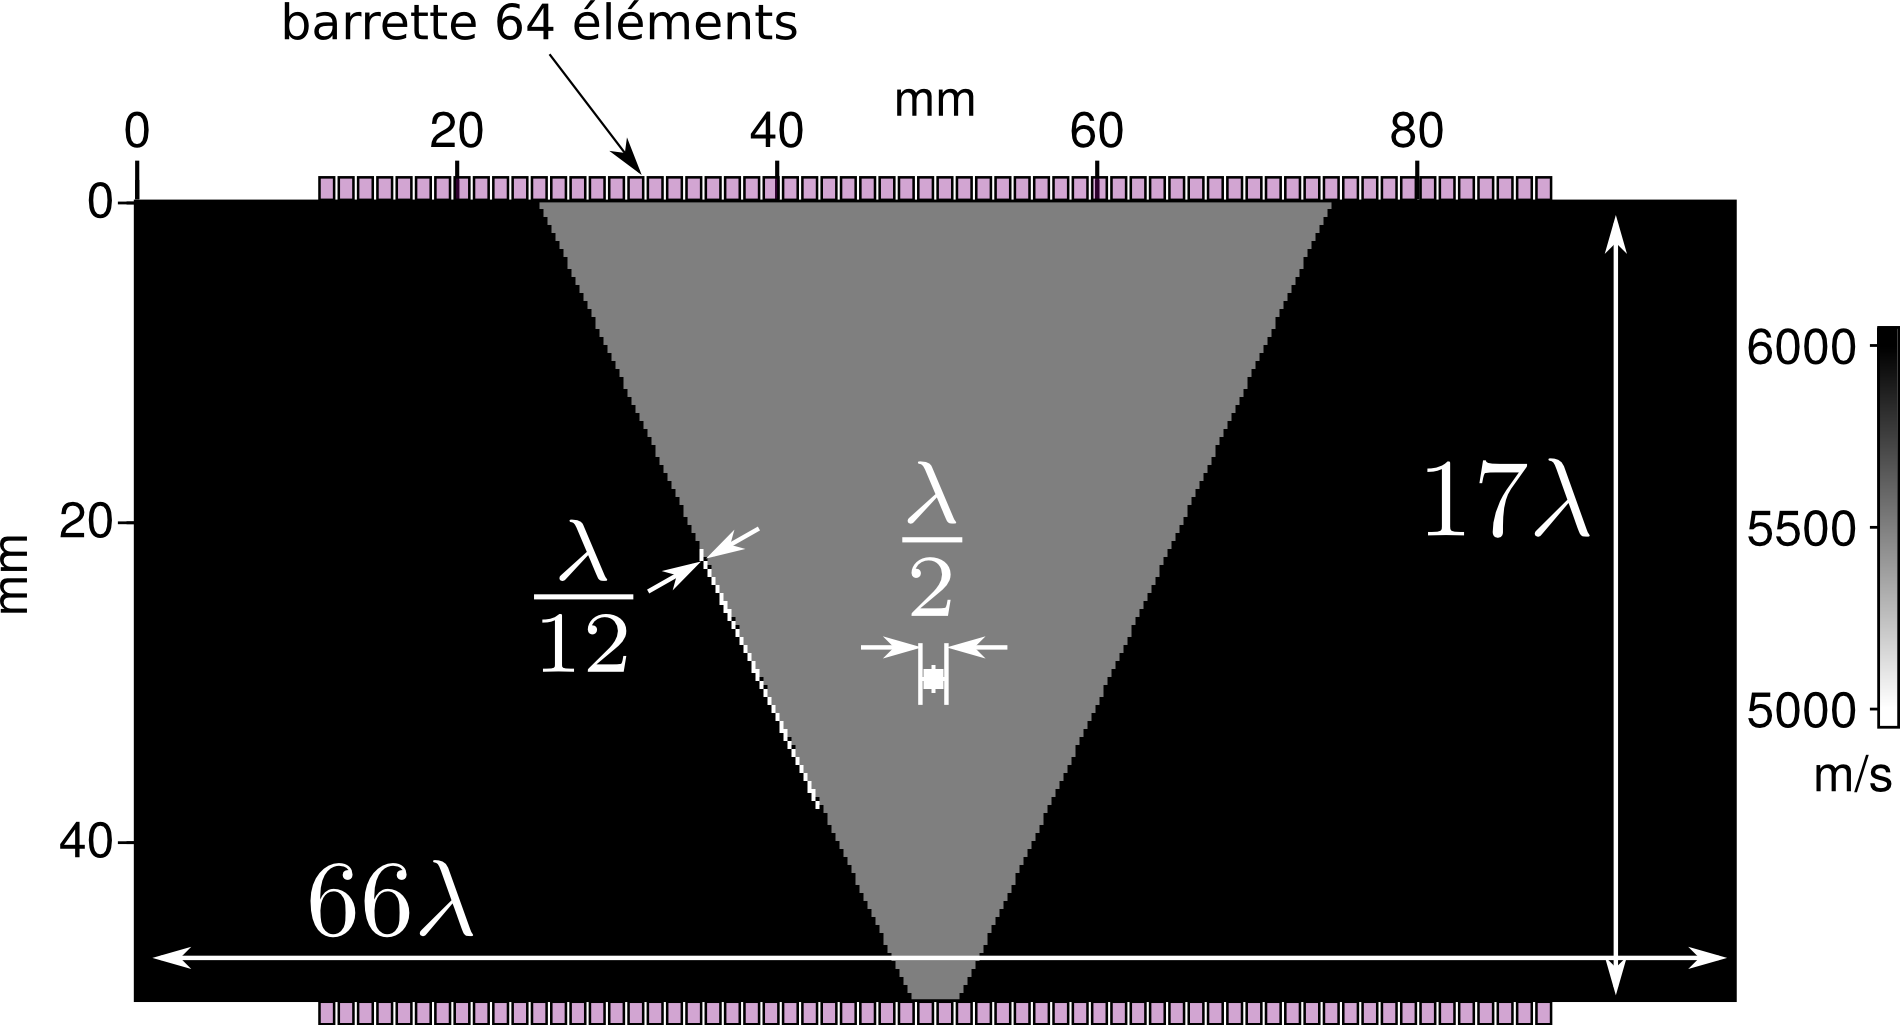
\includegraphics[width=\textwidth]{img/vp_true_lambda.png}\\
			\small{ True velocity}
		\end{figure}
		\column{0.5\textwidth}
		\begin{figure}
			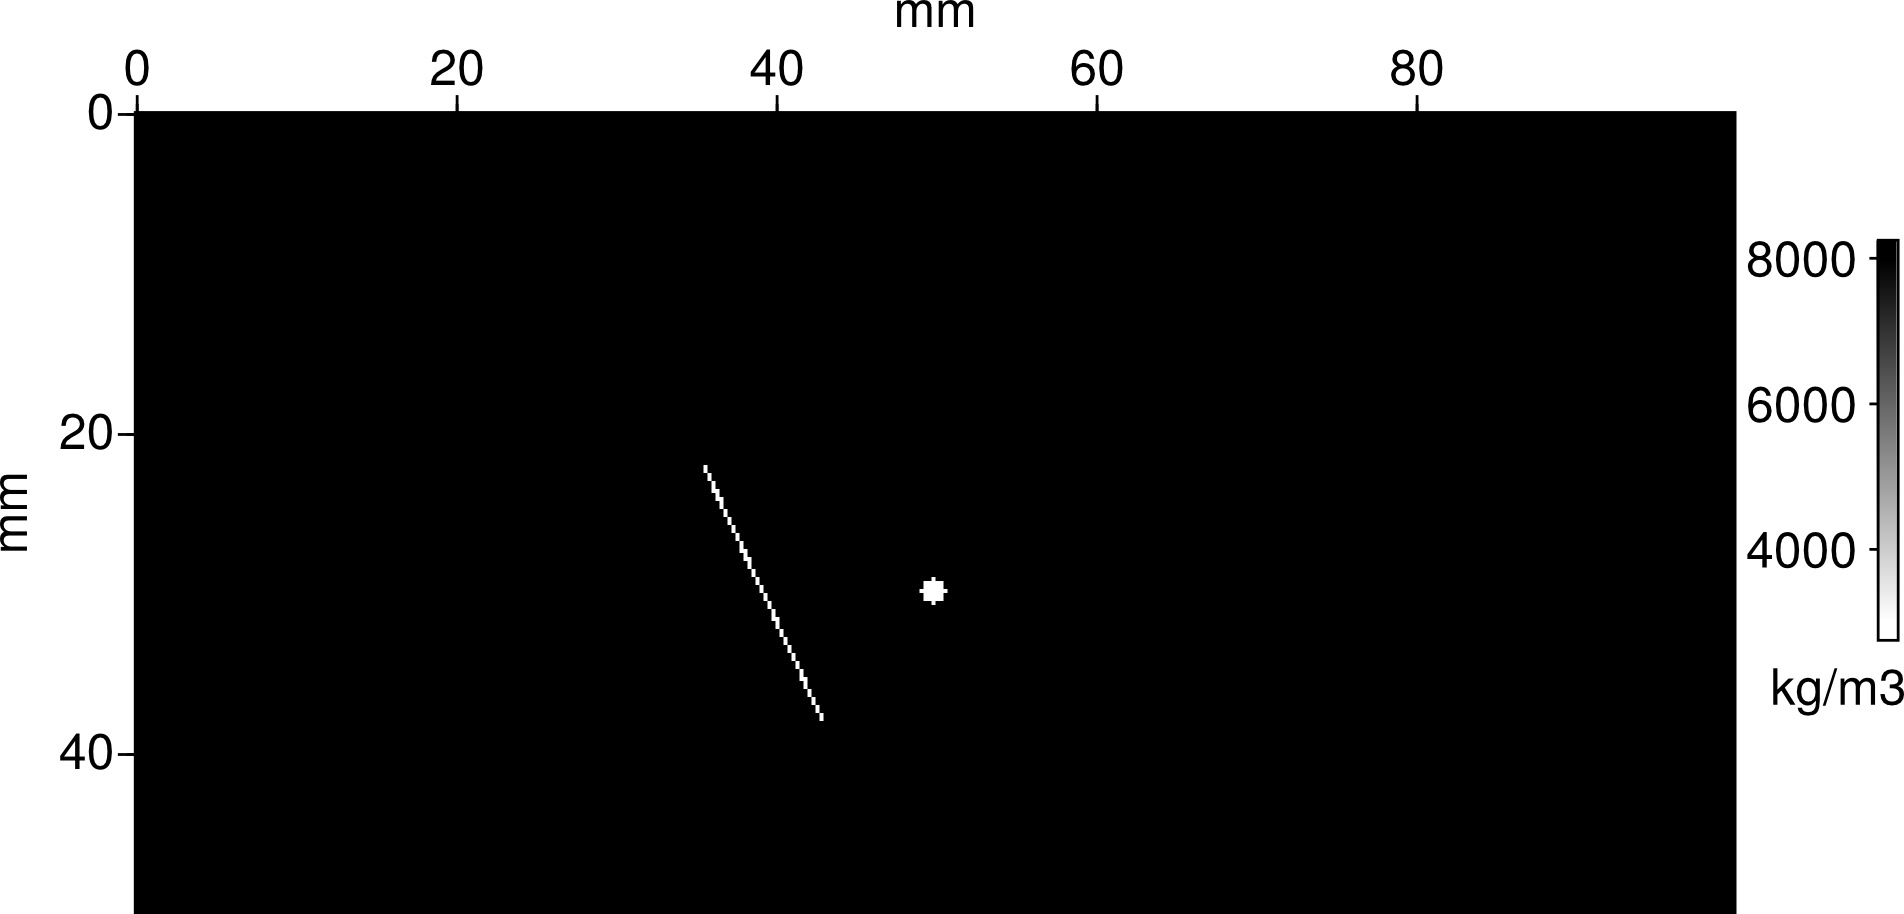
\includegraphics[width=\textwidth]{img/rho_true.png}\\
			\small{ True density}
		\end{figure}
	\end{columns}
	}
	
\end{frame}


\begin{frame}{Transitional model}
	\begin{columns}
	\column{0.5\textwidth}
	Building of a smooth velocy model : 
	\begin{itemize}
		\item from 200 kHz to 1 MHz
		\item strong smoothing of $\bm{\Delta m}$ :  Gaussian on 2 wavelengths
	\end{itemize}
	\column{0.5\textwidth}
		\centering
		\vspace{-1cm}
		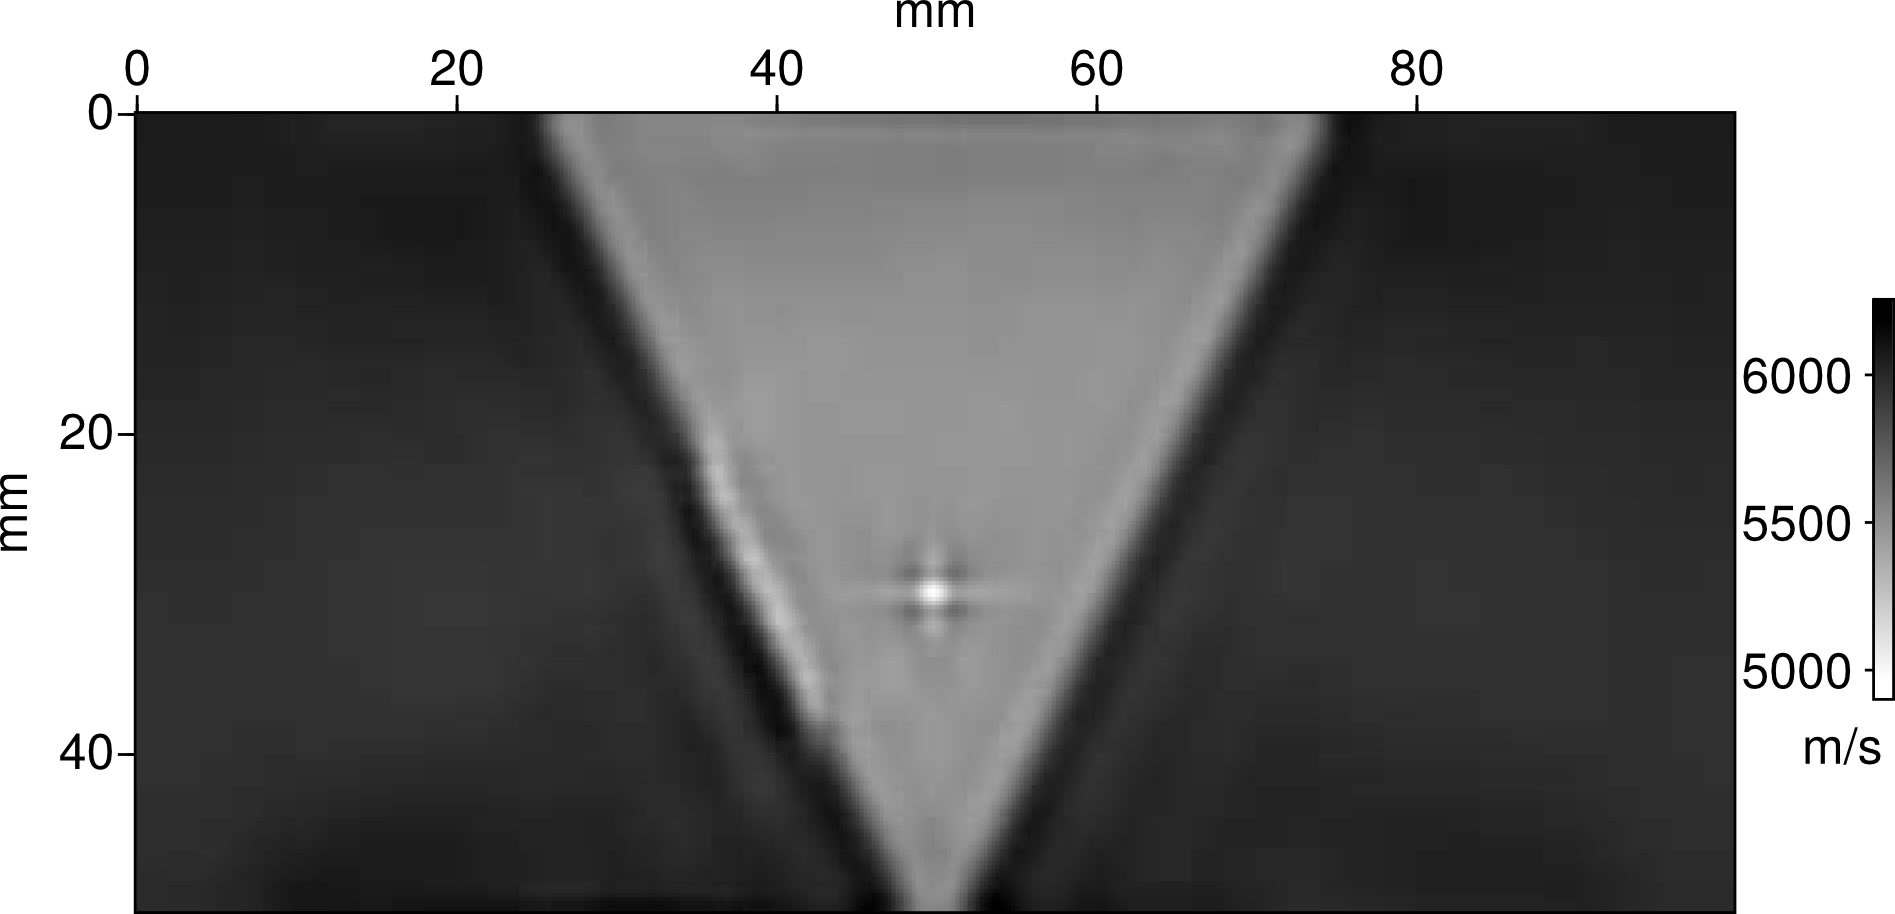
\includegraphics[height=2.7cm]{img/vp_mono_smooth/vp_smooth.png}\\
		\small{Smooth velocity model}
	\end{columns}
	\vspace{0.3cm}
	\begin{columns}
		\column{0.3\textwidth}
		\centering
		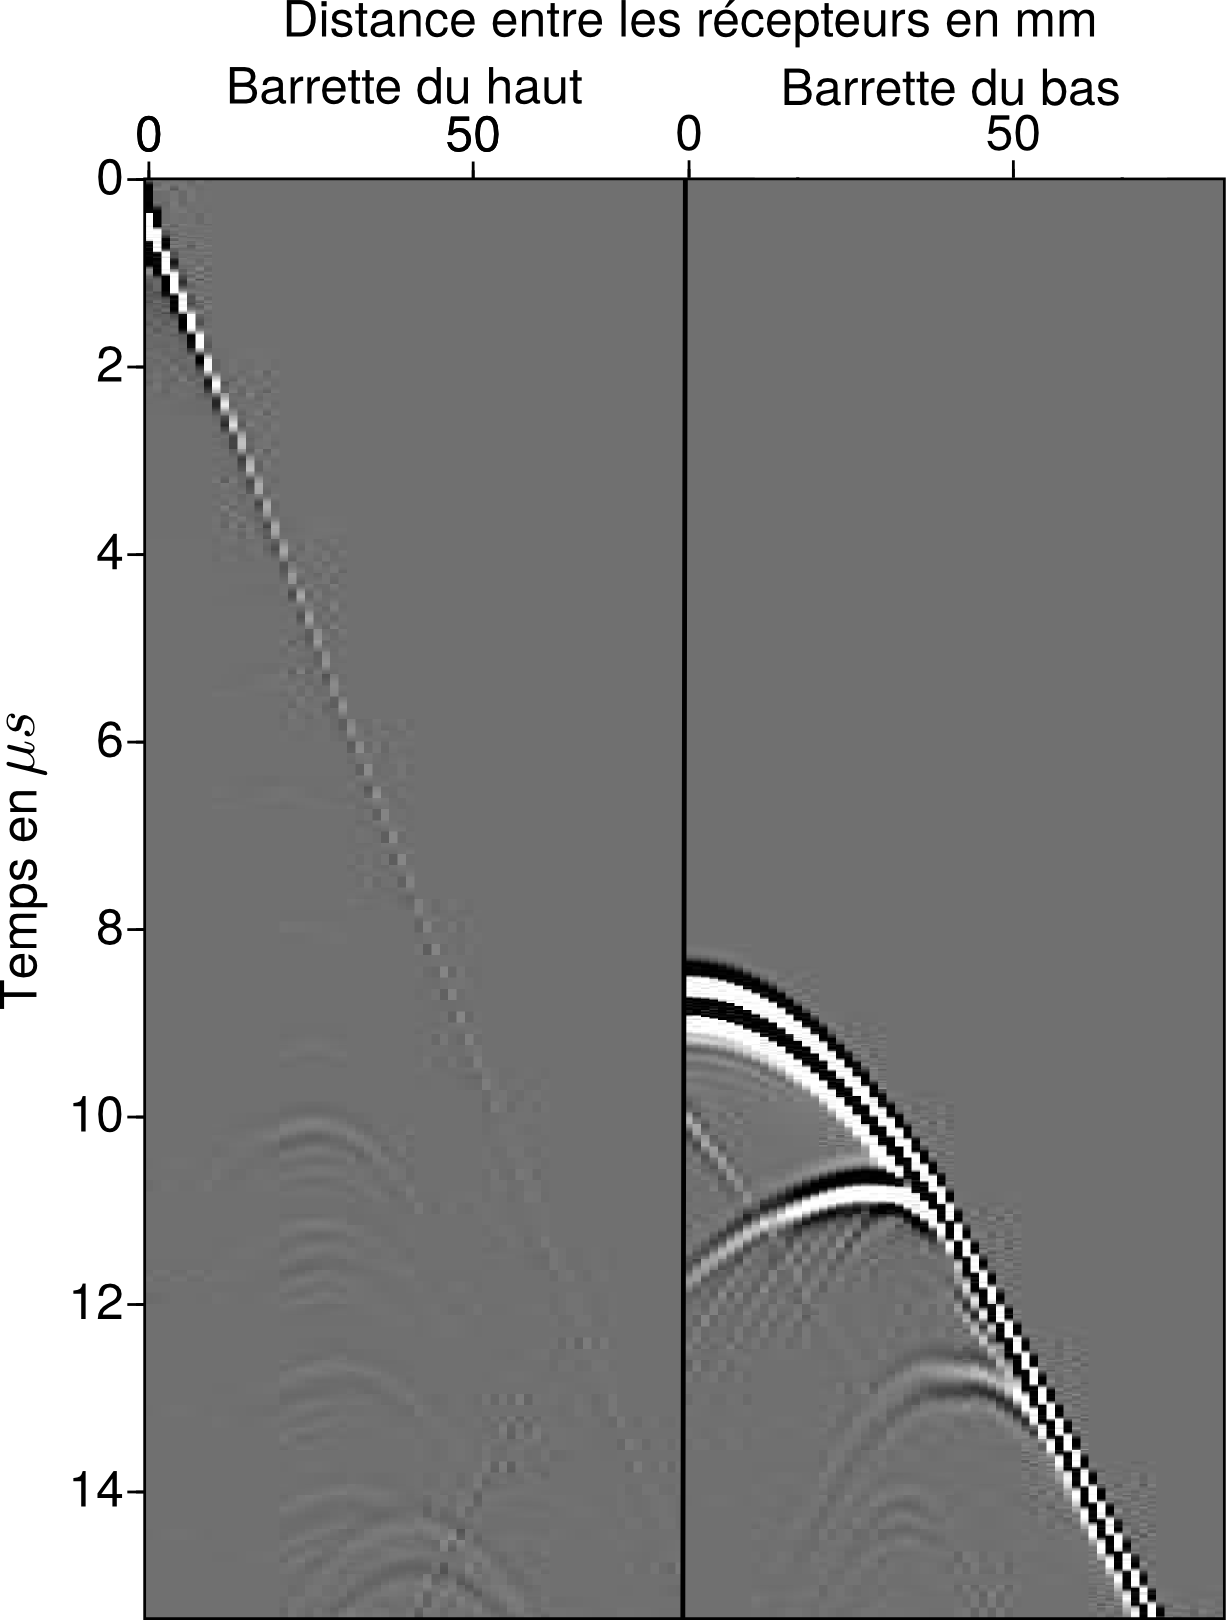
\includegraphics[width=\textwidth]{img/rho_mono/data_rho_uni.png}\\
		\small{Homogeneous density}
		\column{0.3\textwidth}
		\centering
		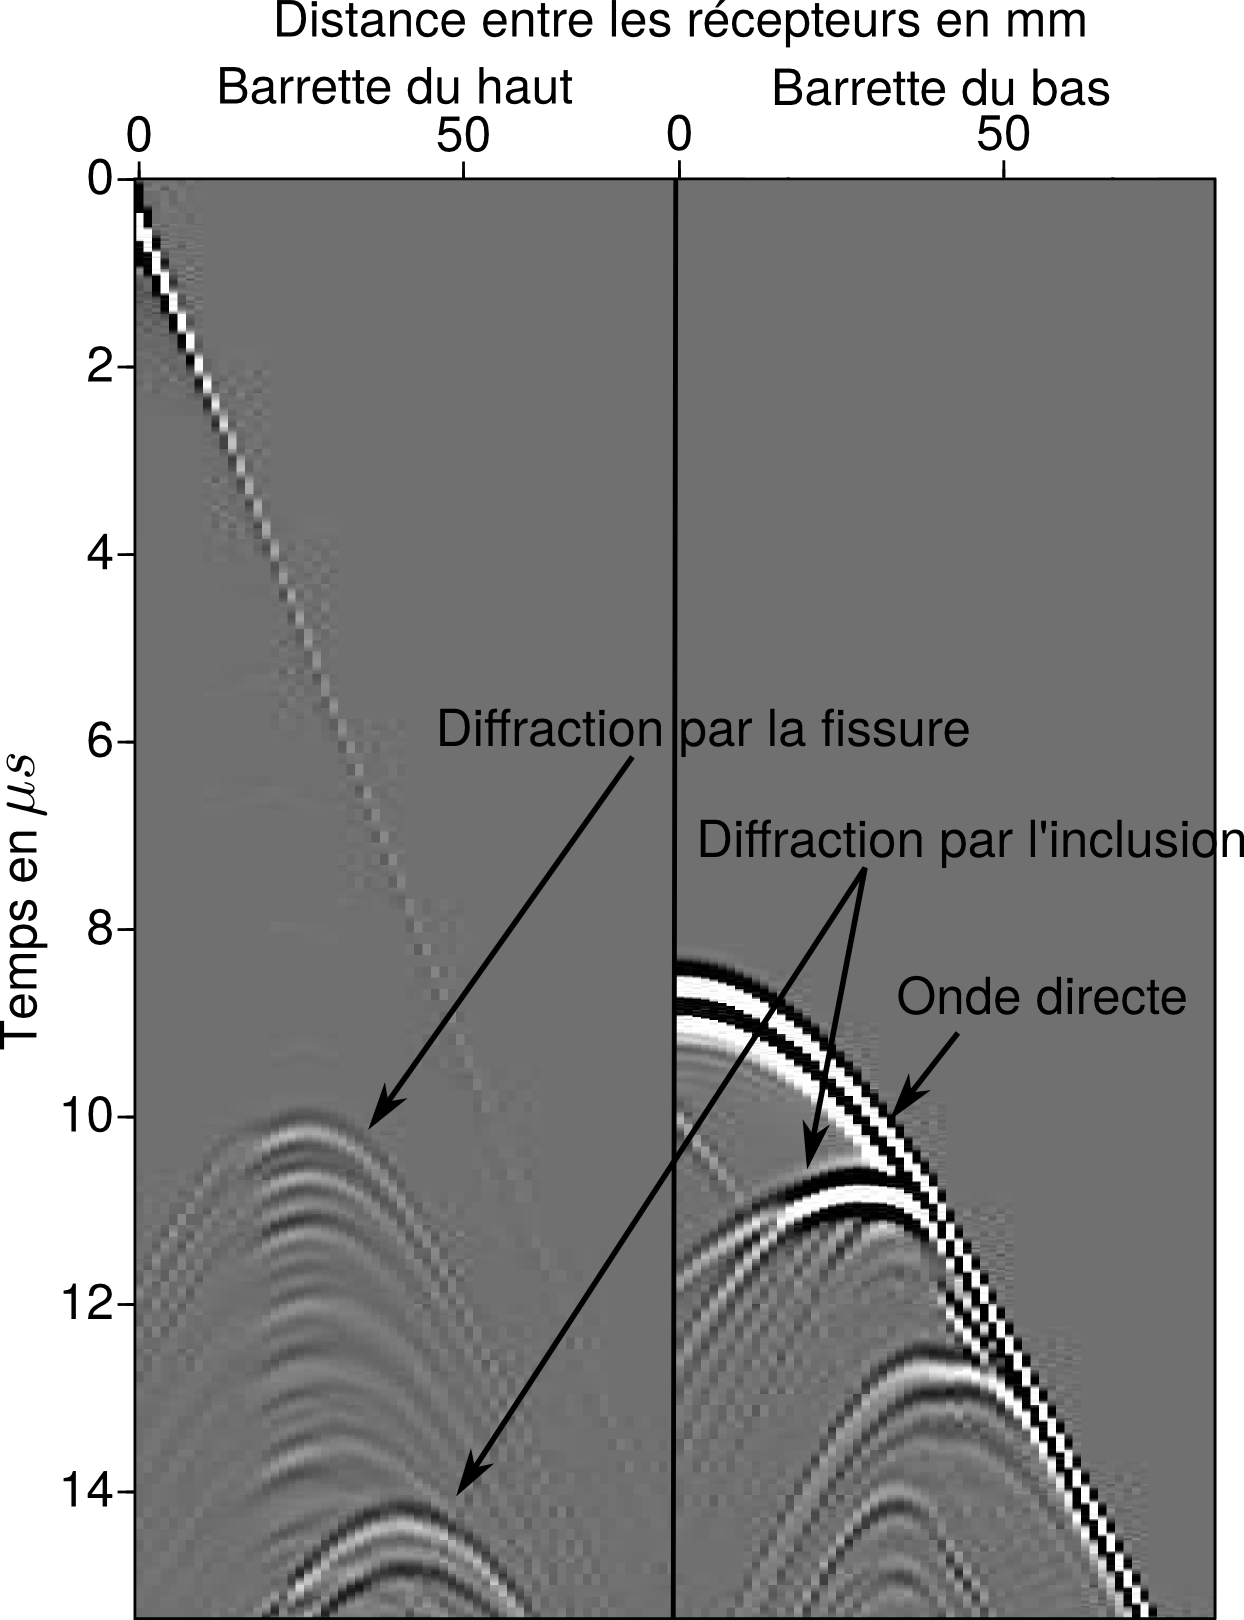
\includegraphics[width=\textwidth]{img/rho_mono/data_rho_vrai.png}\\
		\small{True density}
	\end{columns}
	
	
\end{frame}

\begin{frame}{Isotropic case}
\setlength{\leftmargin}{-2cm}
\setlength{\rightmargin}{-2cm}
%\setlength{\textwidth}{29cm}
\begin{picture}(0,0)(0,0)\put(-20,-90){
	$v_{p}$
}\end{picture}
\begin{picture}(0,0)(0,0)\put(-20,-160){
	$\rho$
}\end{picture}
\begin{itemize}
	\item 9 succesive inversions from 200 kHz to 3 MHz 
\end{itemize}
\vspace{1cm}

	\begin{columns}
		\column{0.3\textwidth}
		\centering
		\small{Initial \\ model}
		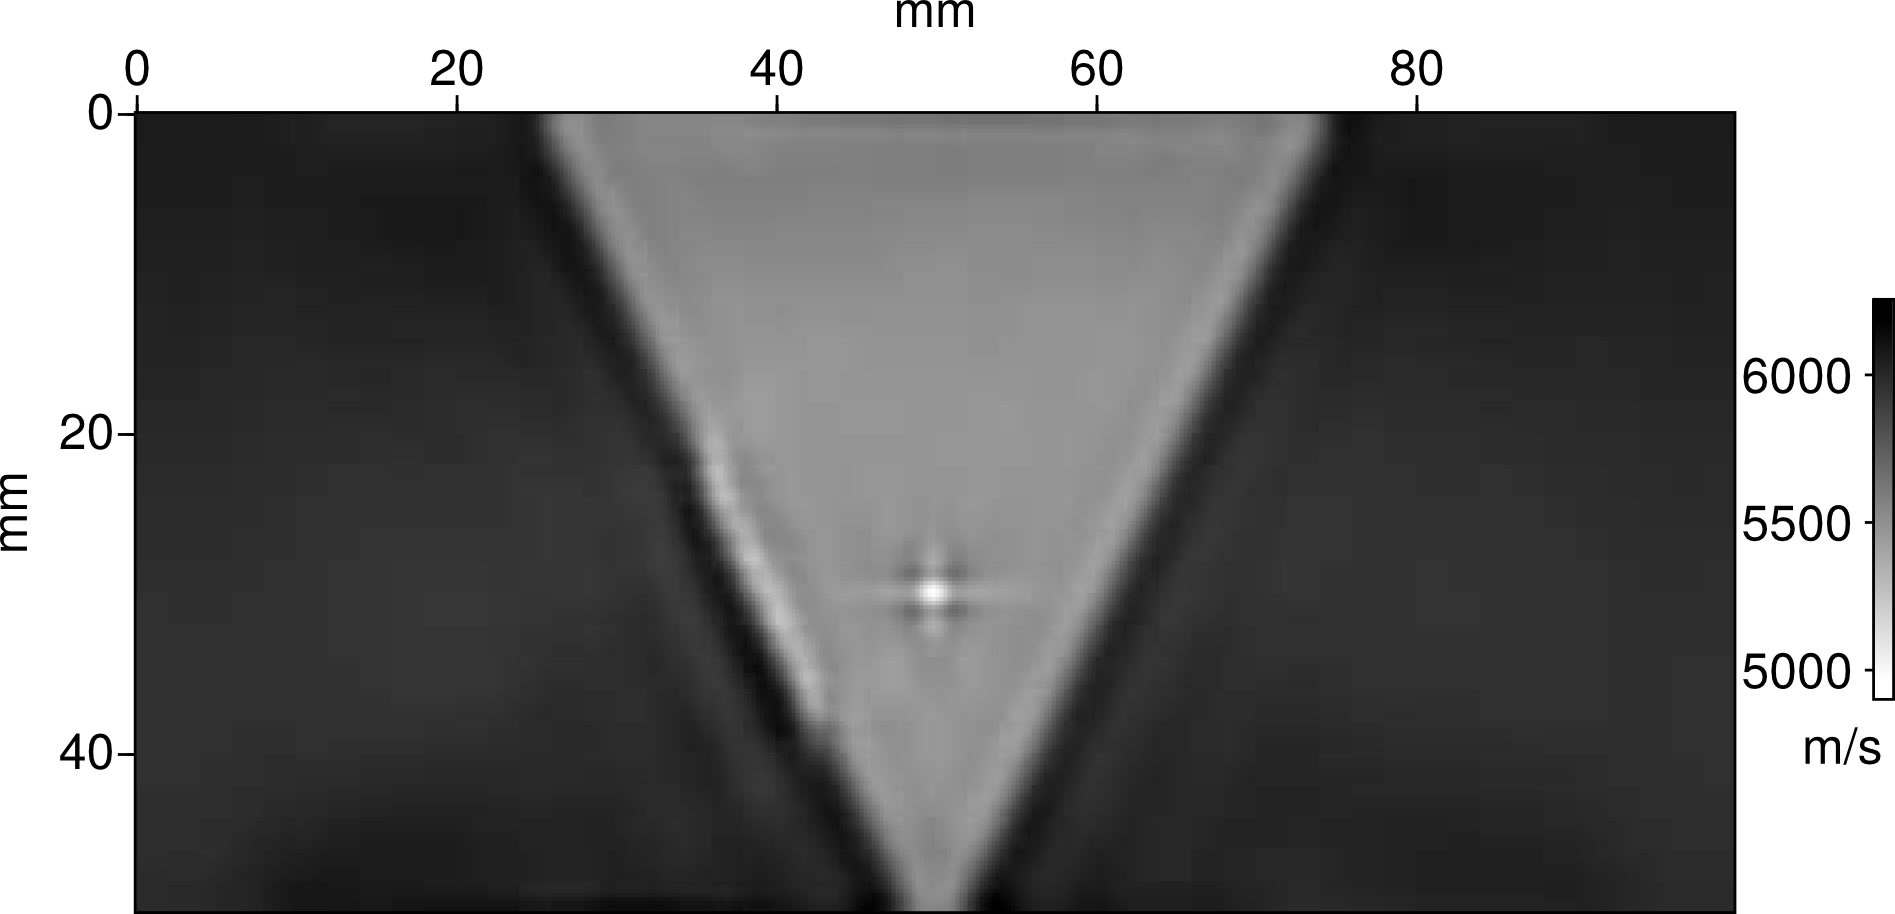
\includegraphics[height=1.9cm]{img/vp_mono_smooth/vp_smooth.png}\\
		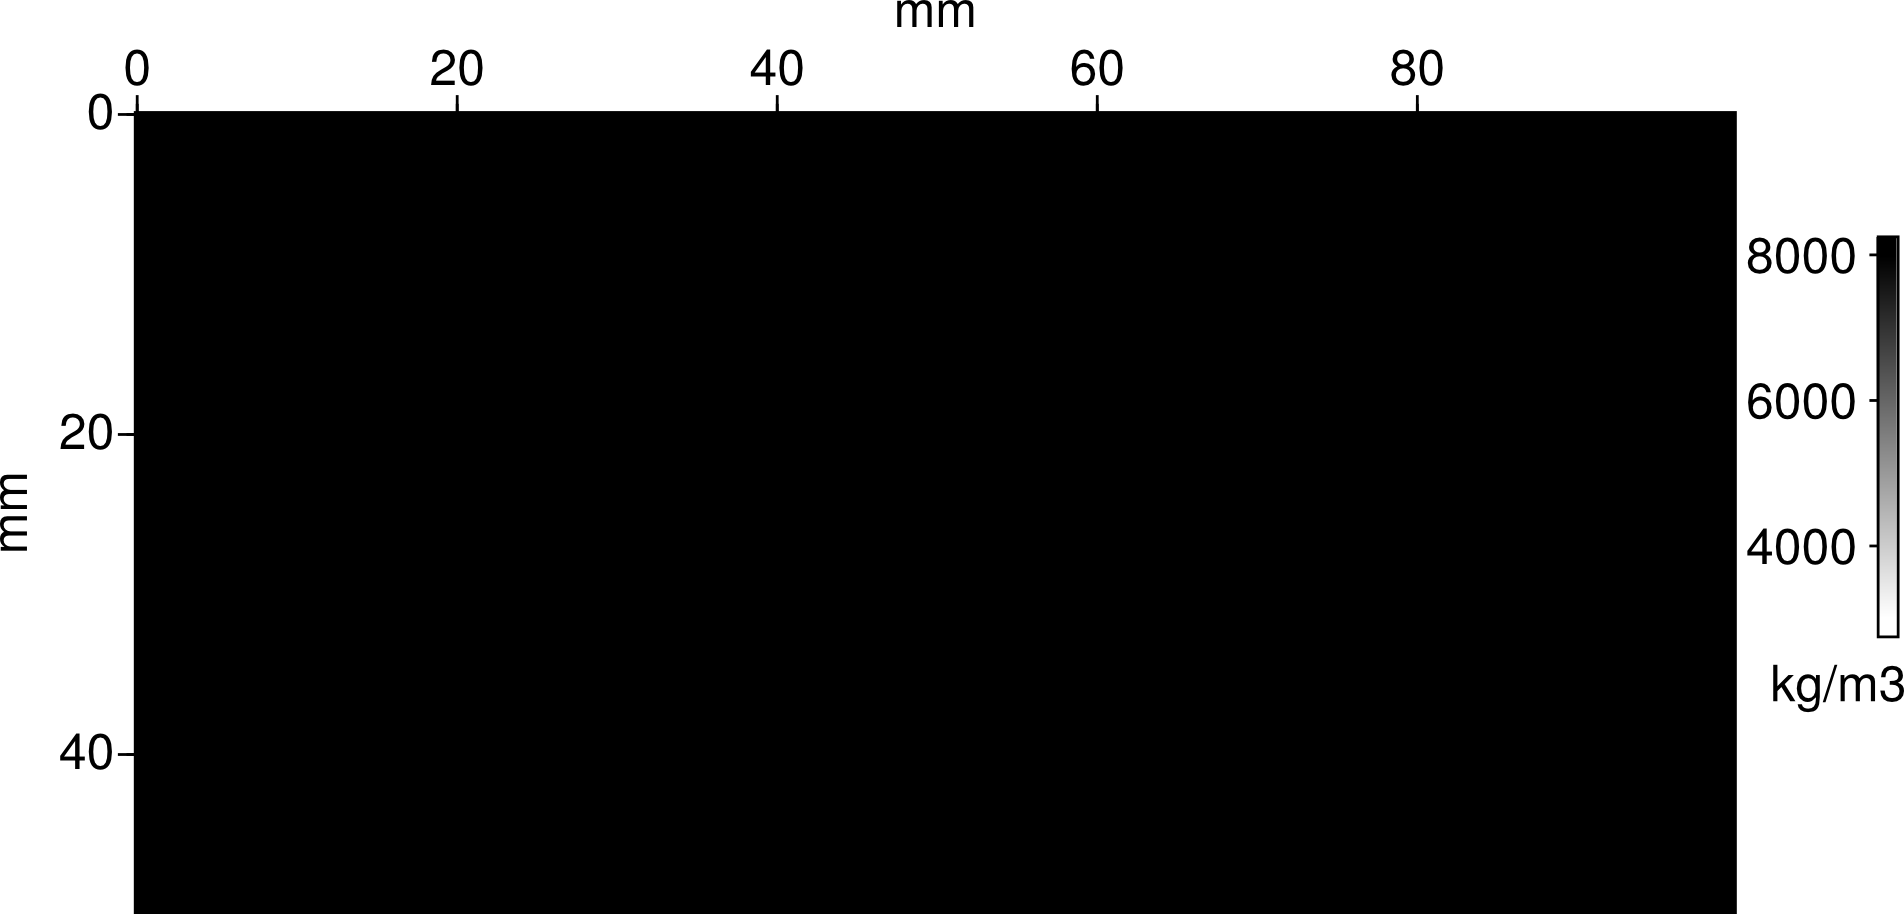
\includegraphics[height=1.9cm]{img/rho_mono/rho_init.png}		
		\column{0.3\textwidth}
		\centering
		\small{Monoparameter inversion}
		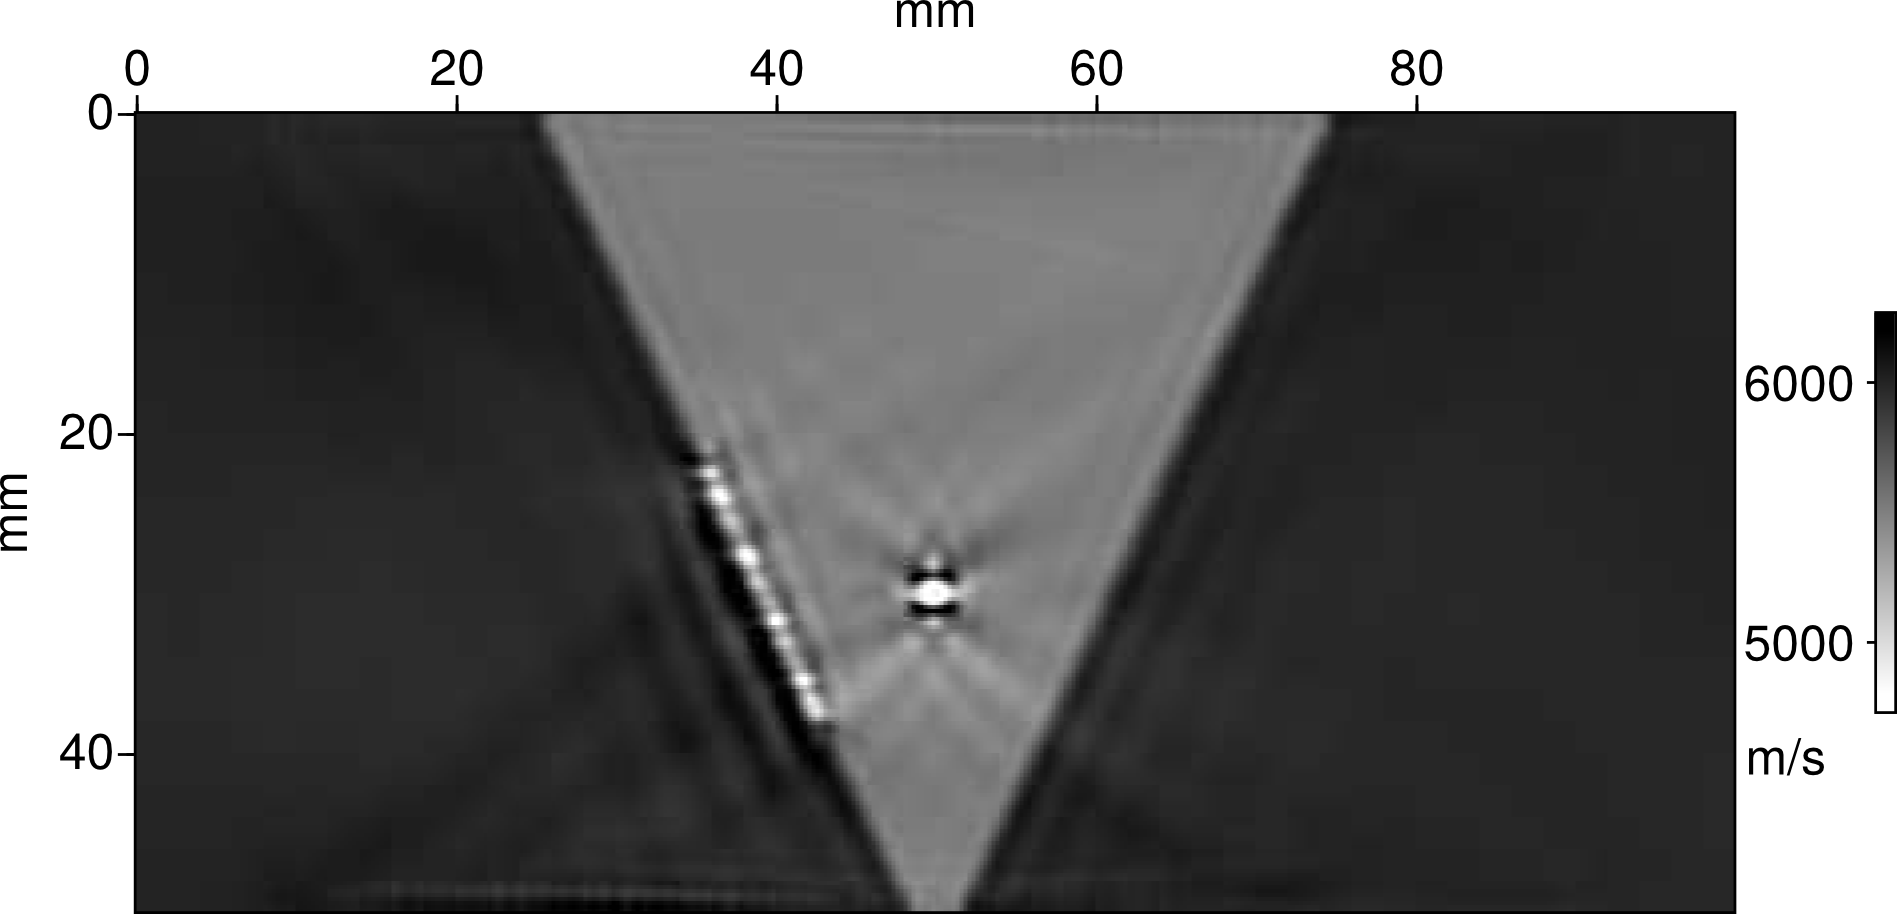
\includegraphics[height=1.9cm]{img/vp_mono_uni/vp_3300k.png}\\
		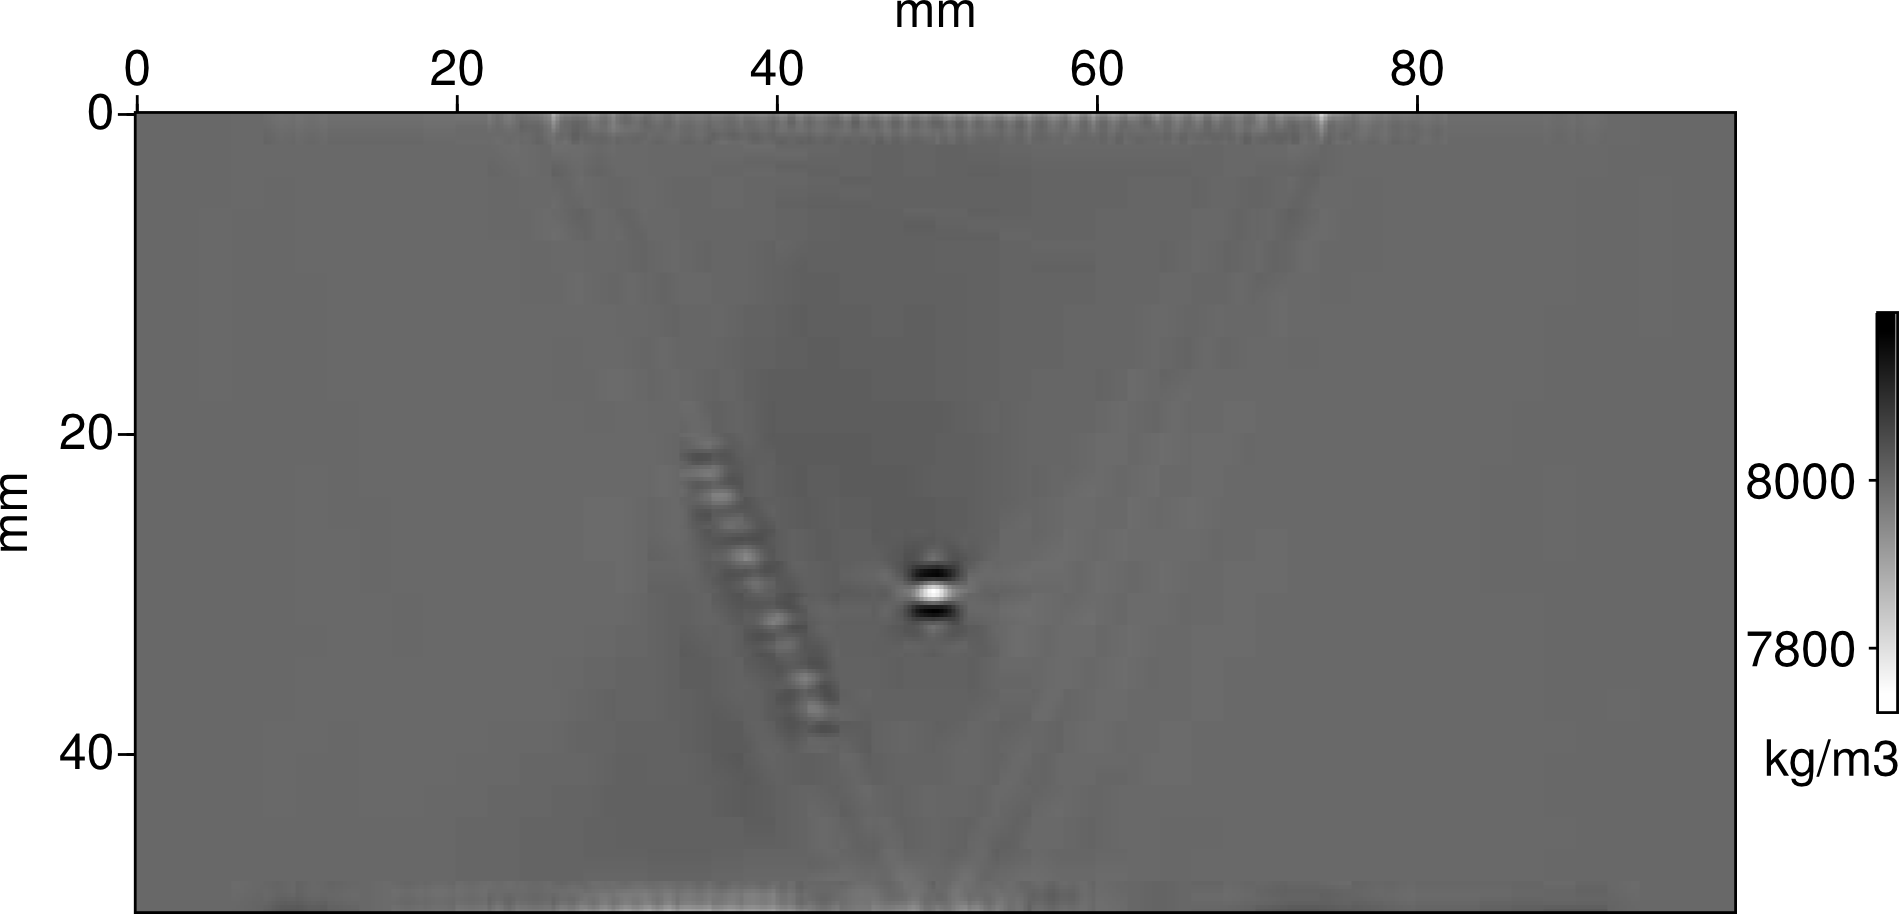
\includegraphics[height=1.9cm]{img/rho_mono/rho_mono.png}		
		\column{0.3\textwidth}
		\centering
		\small{Multiparameter inversion}
		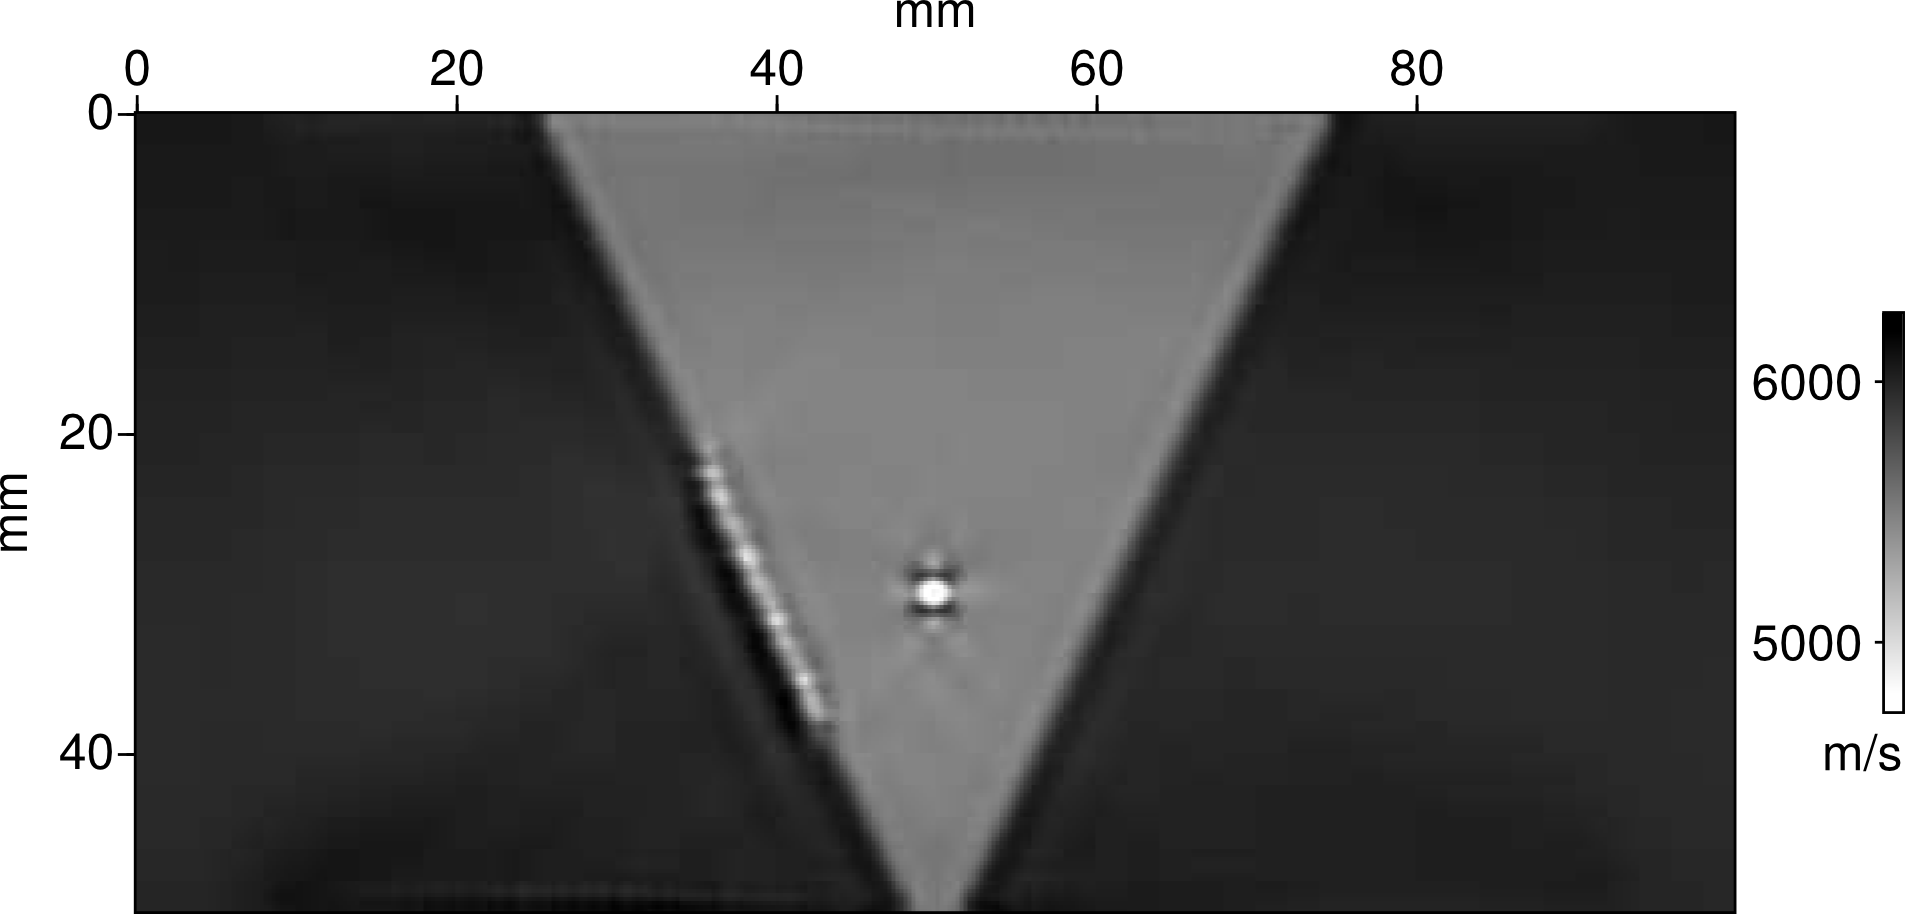
\includegraphics[height=1.9cm]{img/multi/vp_multi_6000k.png}\\		
		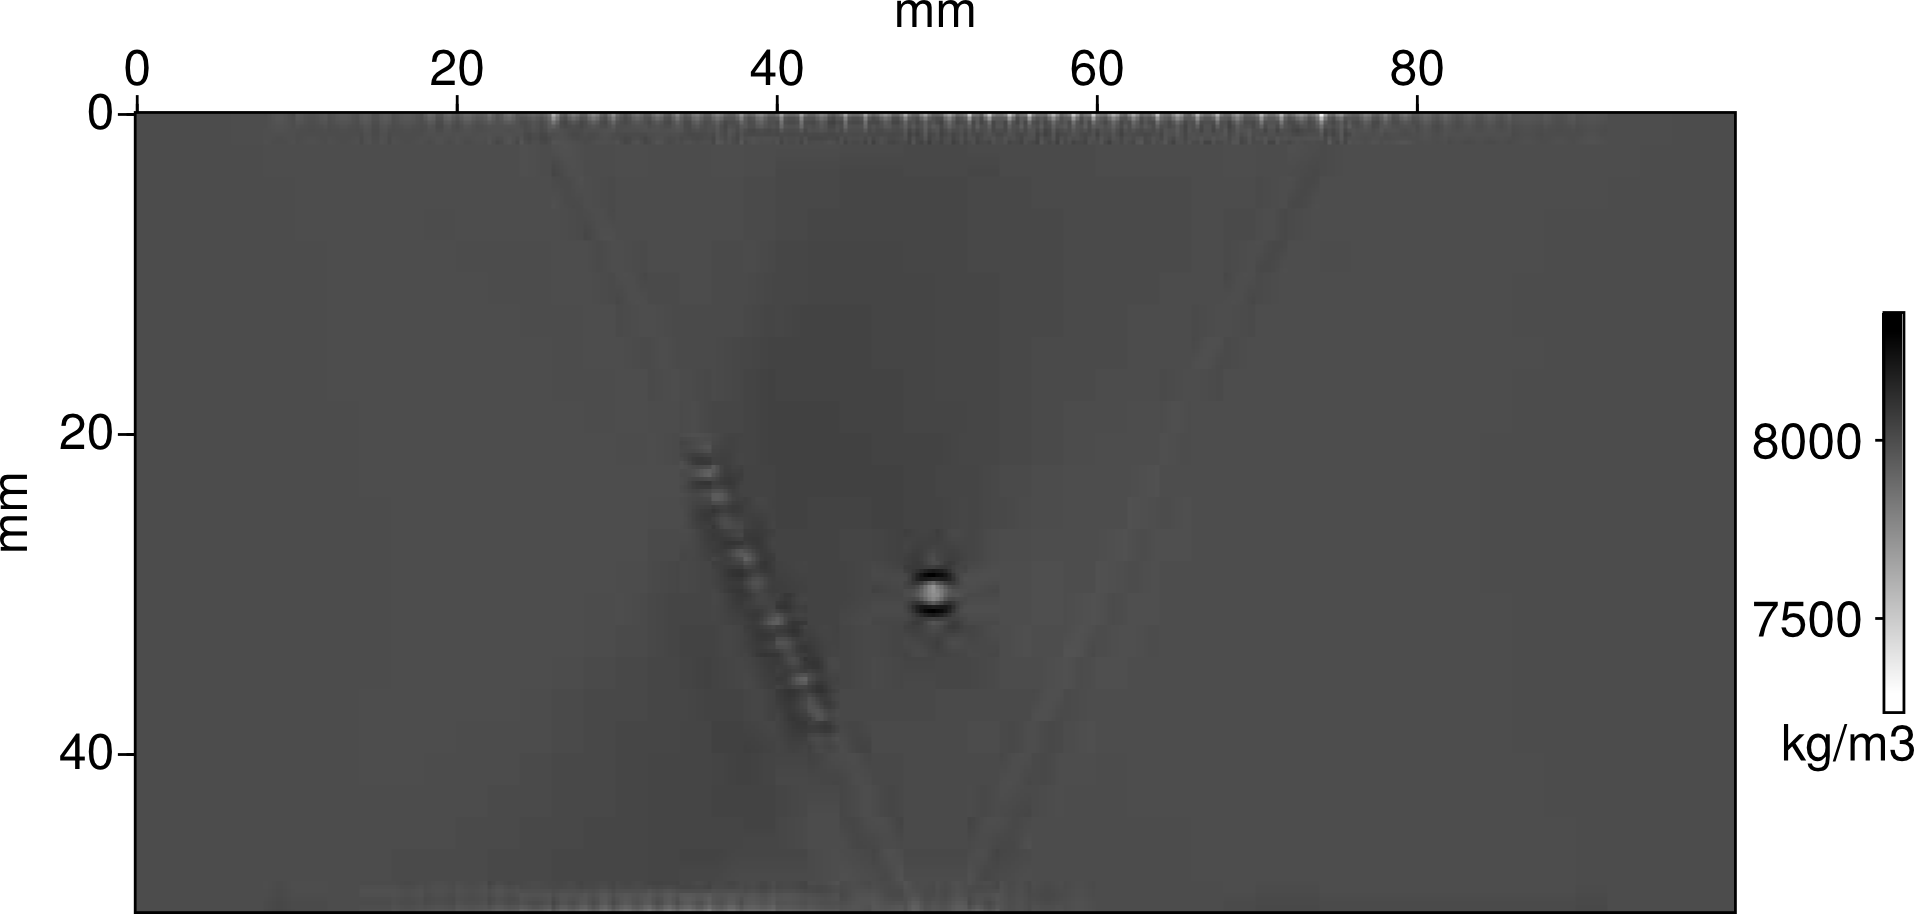
\includegraphics[height=1.9cm]{img/multi/rho_6000k.png}\\		
	\end{columns}
\end{frame}


%\subsection{Inversion monoparamètre}
%\begin{frame}{\insertsectionhead~-- Vitesse}
%\begin{small}
%\centering
%	\begin{adjustwidth}{-2em}{-2.5em}
%	%\centering{Reconstruction de la vitesse}
%	\begin{columns}
%		\column{0.5\textwidth}
%		\centering
%		\vspace{0.1cm}\\	
%		Modèle initial de vitesse : \\[0.2cm]
%		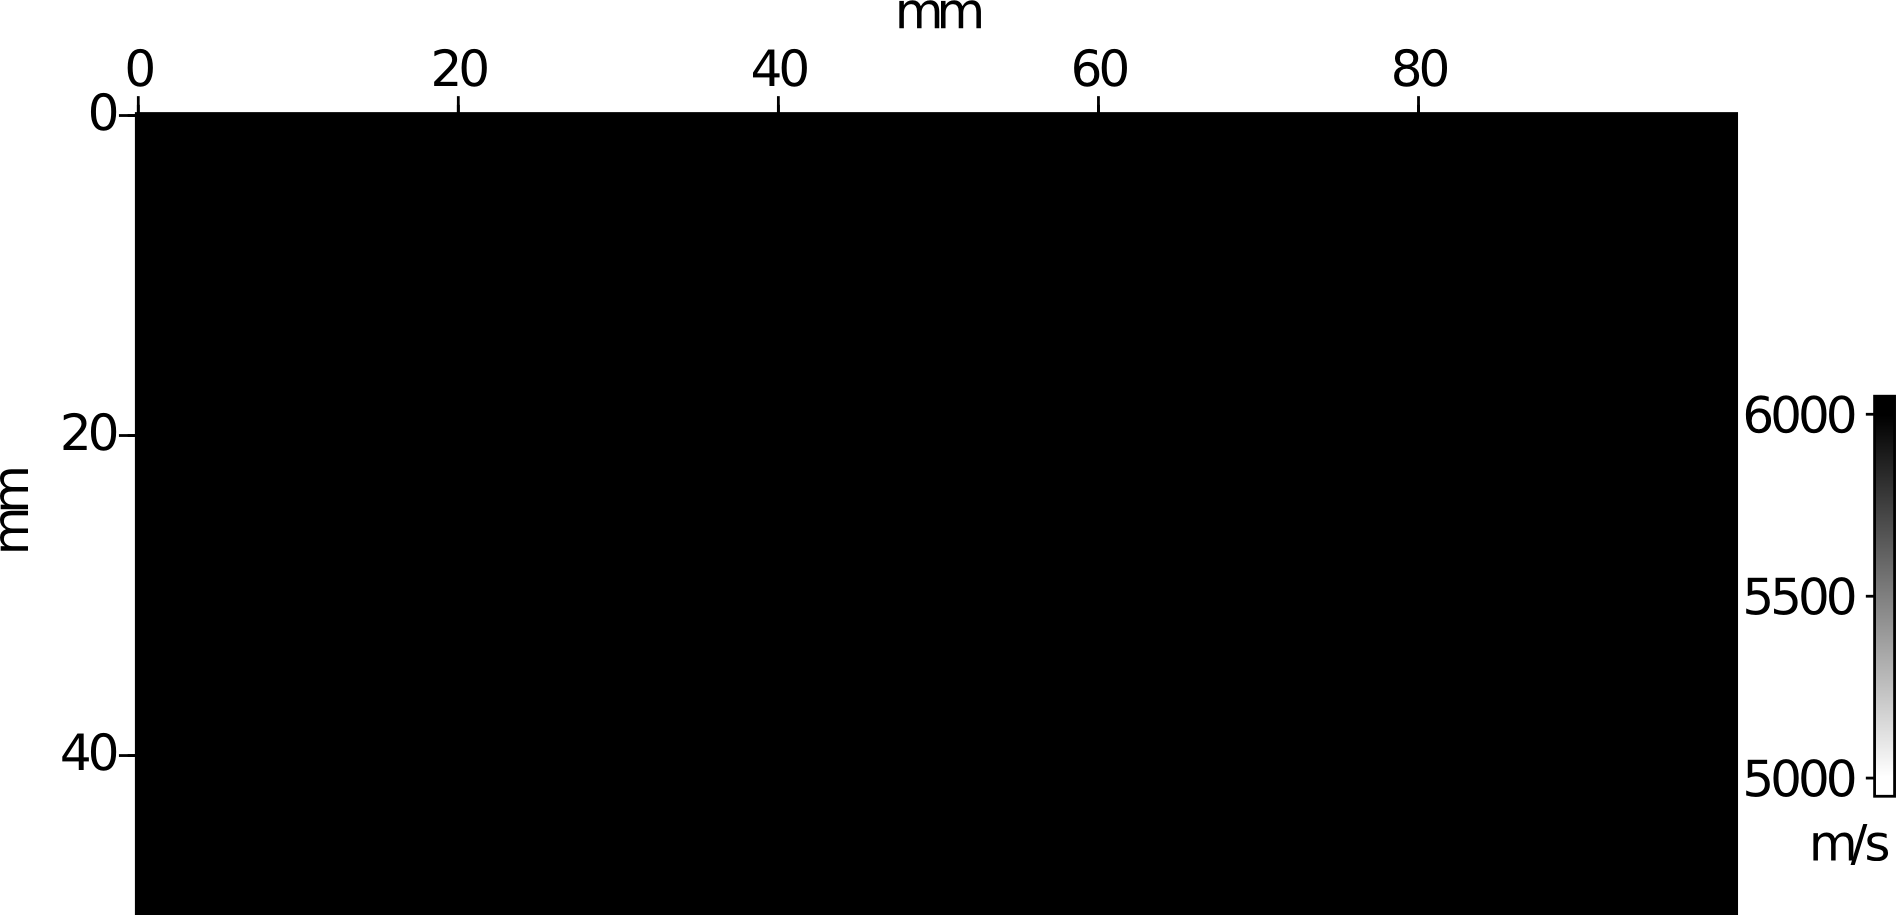
\includegraphics[width=0.7\textwidth]{img/vp_mono_uni/vp_uni.png}\\
%			\only<2->{\vspace{0.3cm}  Vitesse Reconstruite :\\[0.2cm]}
%			\only<1-1>{\vspace{2.7cm}}
%			\only<2-2>{
%				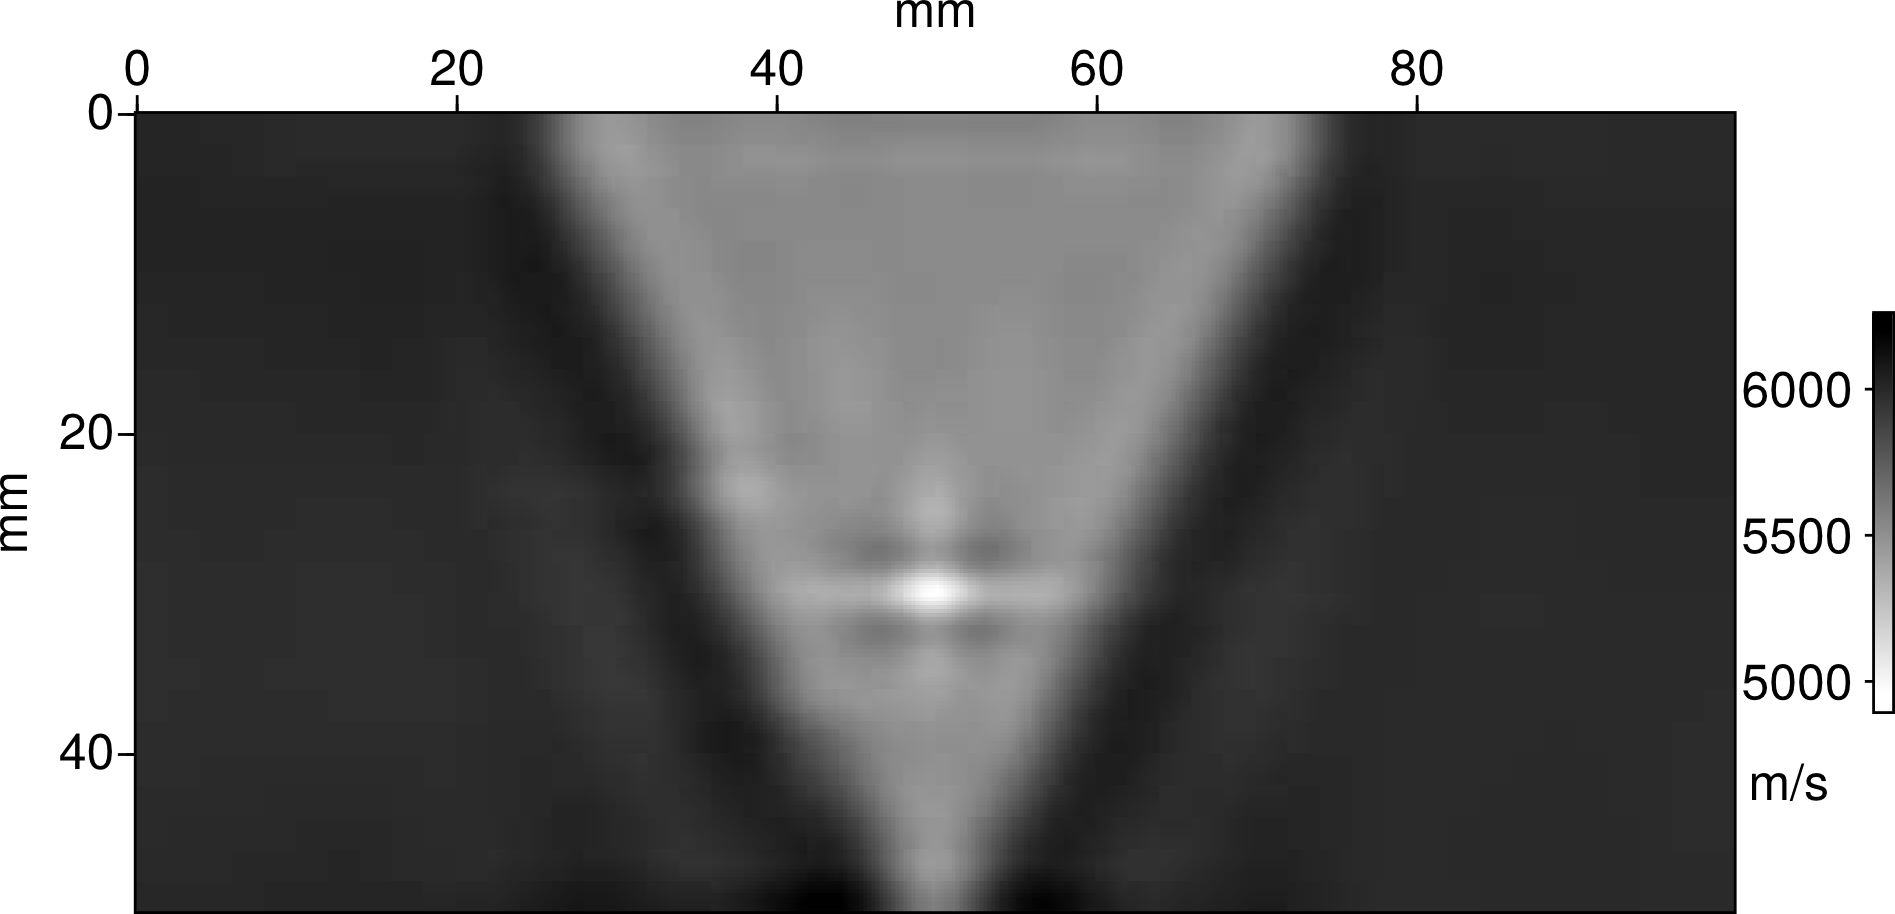
\includegraphics[width=0.7\textwidth]{img/vp_mono_uni/vp_450k.png}\\		
%			}
%		
%			\only<3-3>{
%				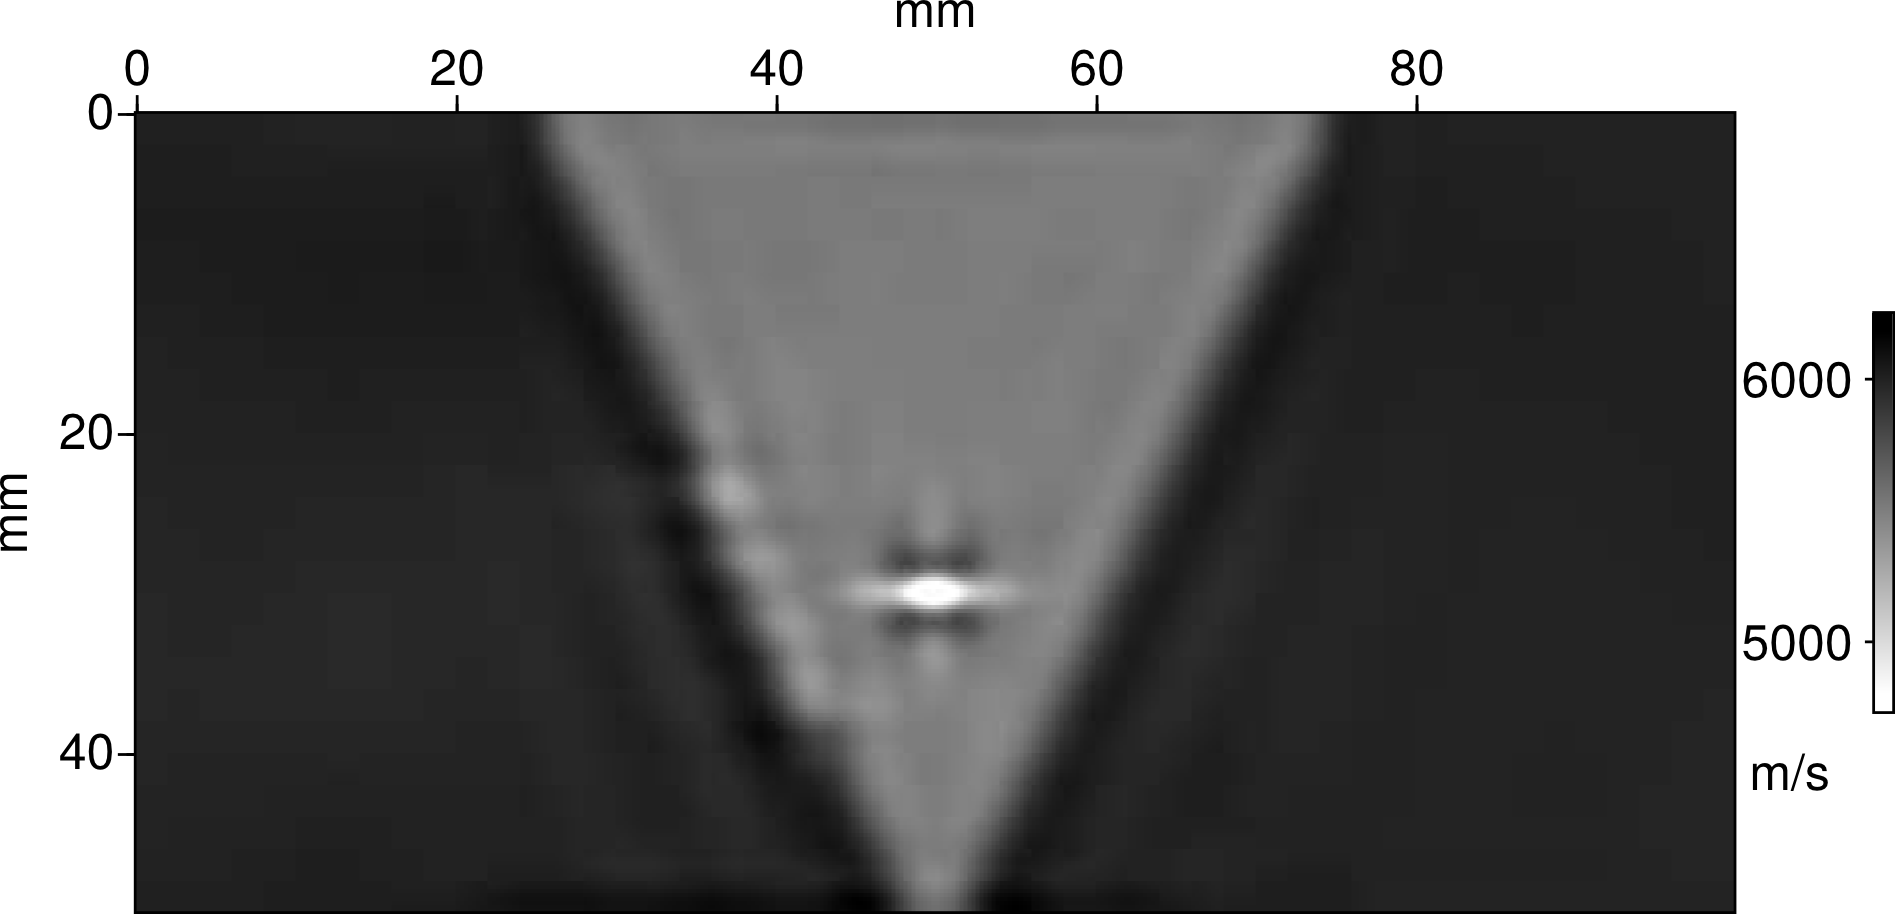
\includegraphics[width=0.7\textwidth]{img/vp_mono_uni/vp_1000k.png}\\		
%			}
%			\only<4-4>{
%				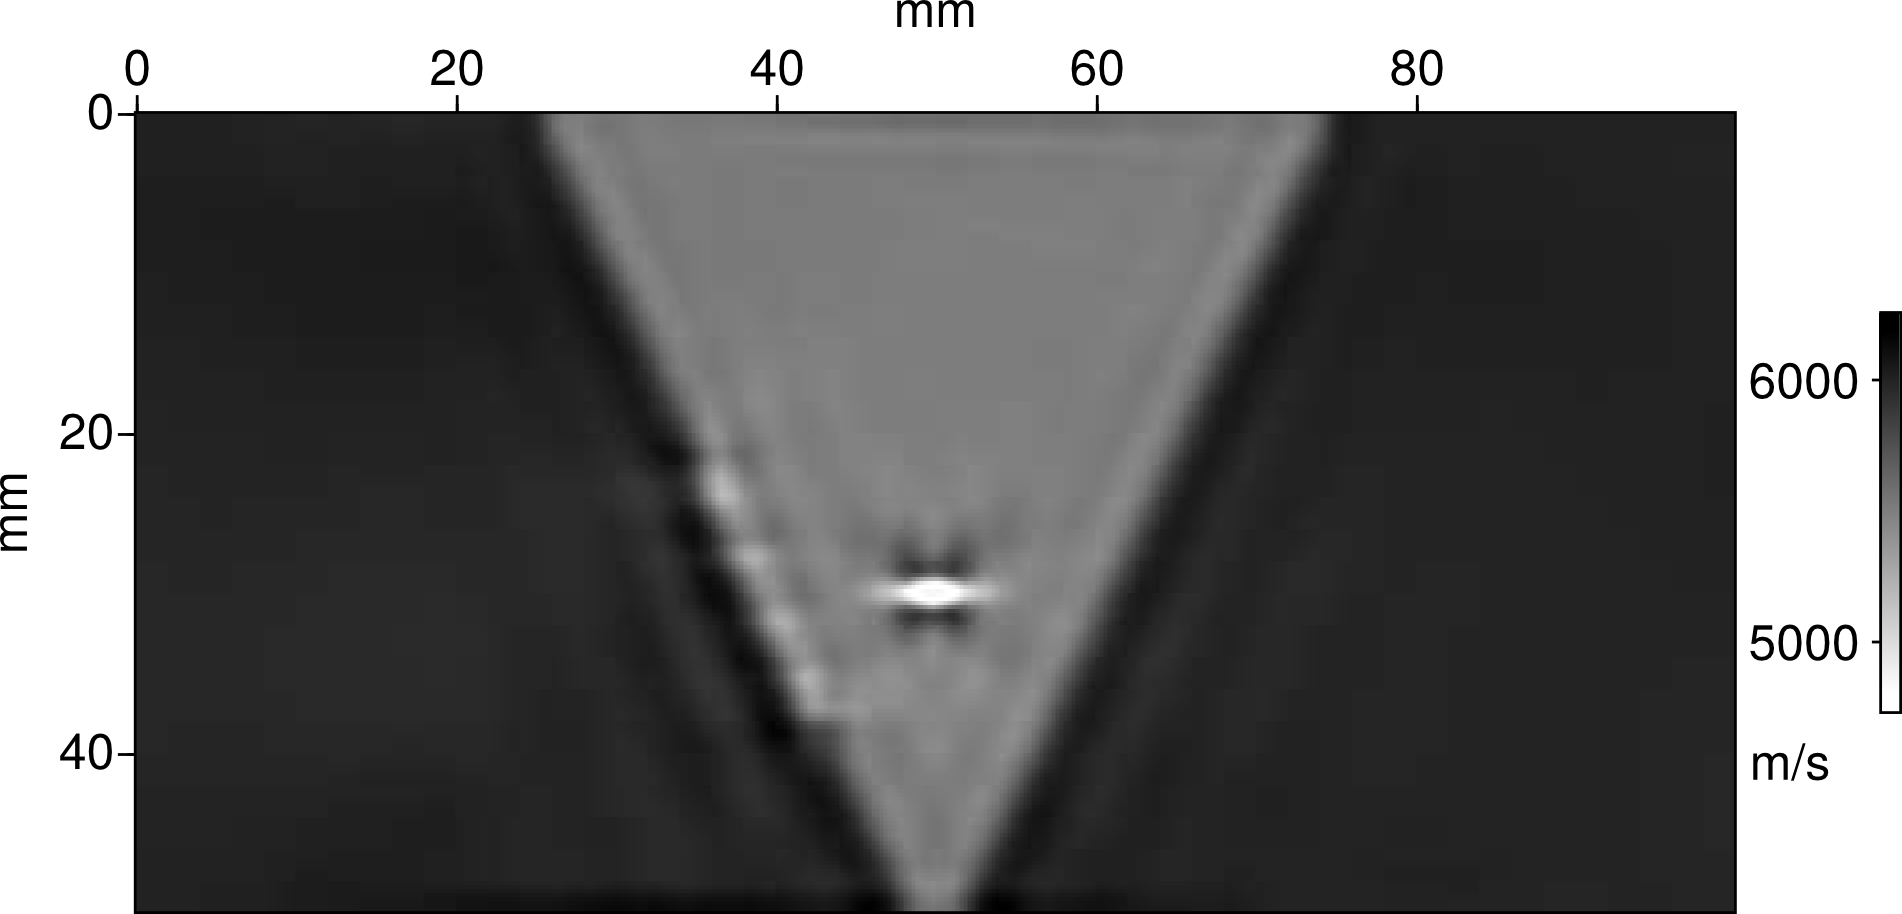
\includegraphics[width=0.7\textwidth]{img/vp_mono_uni/vp_1500k.png}\\		
%			}
%			\only<5-5>{
%				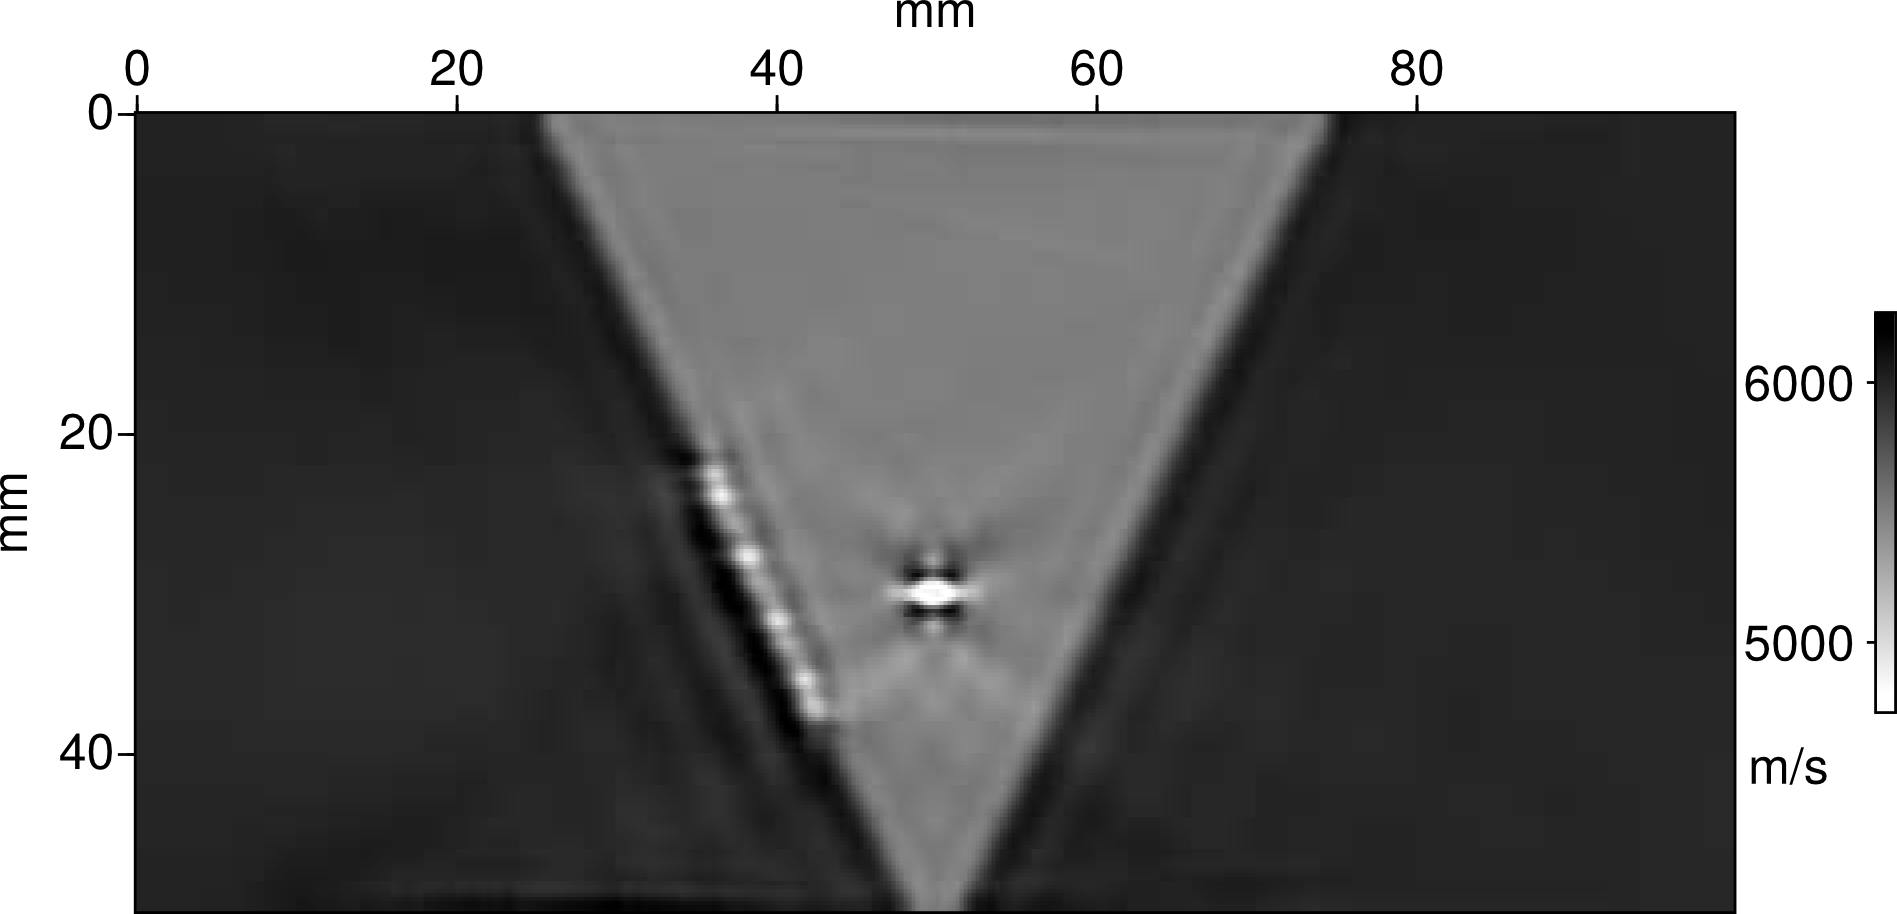
\includegraphics[width=0.7\textwidth]{img/vp_mono_uni/vp_2250k.png}\\		
%			}
%			\only<6->{
%				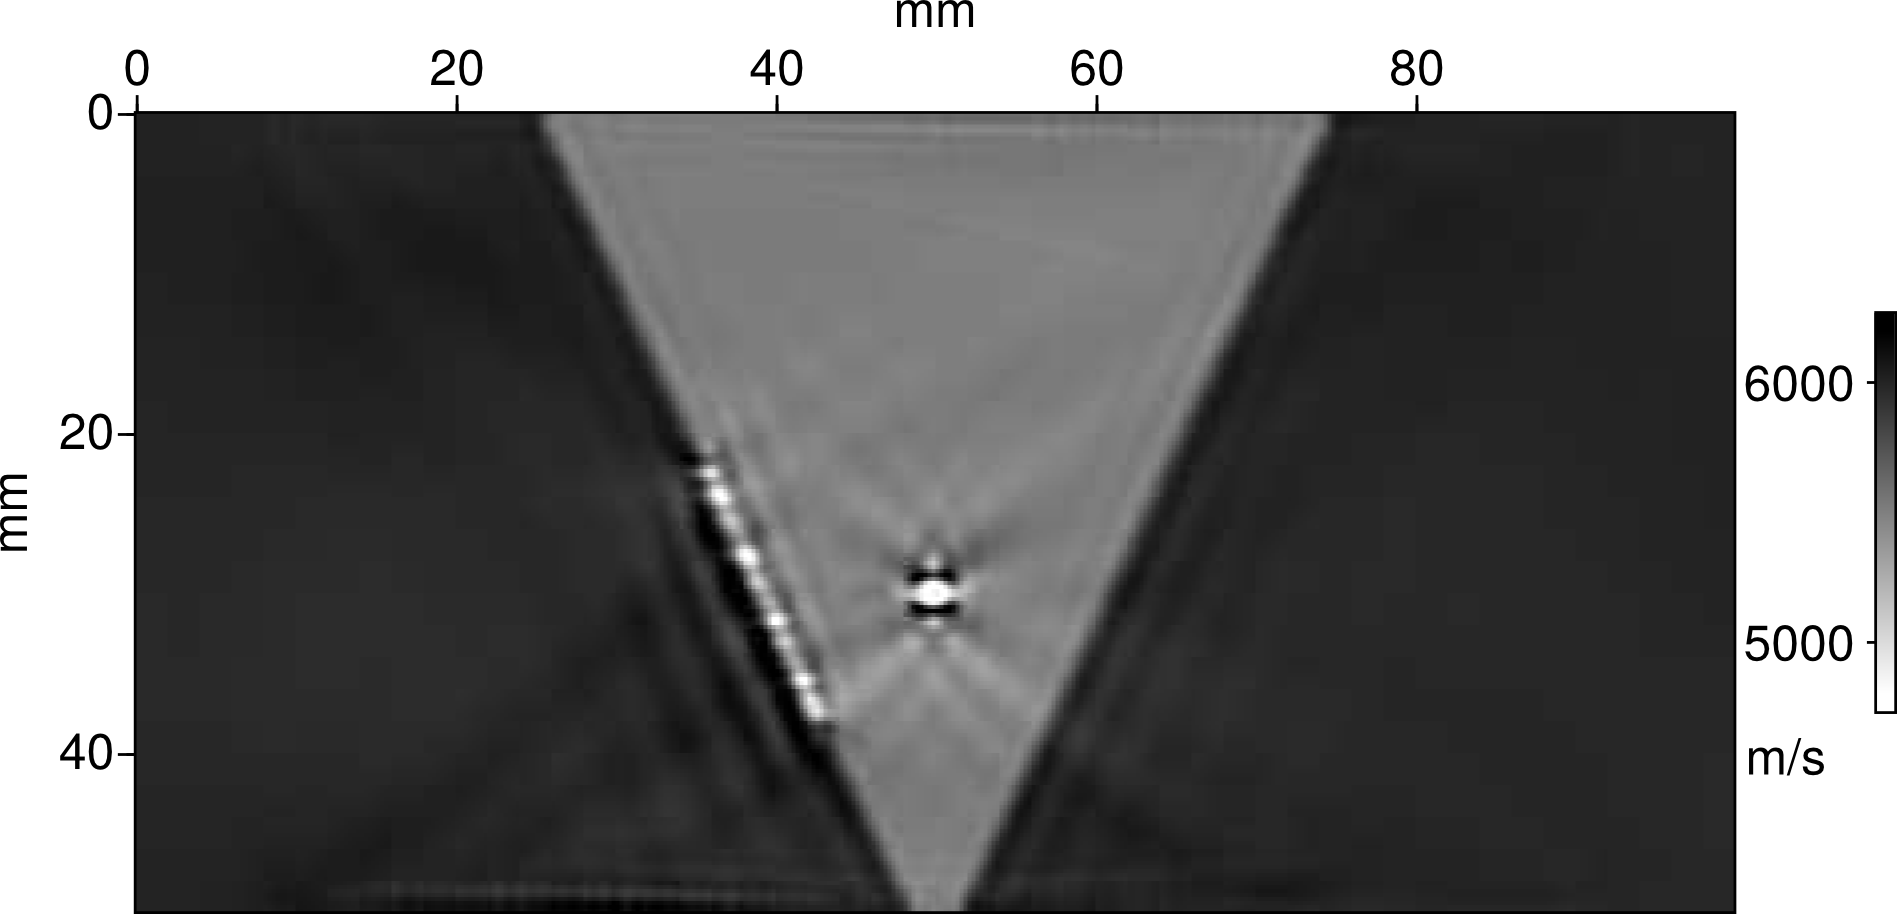
\includegraphics[width=0.7\textwidth]{img/vp_mono_uni/vp_3300k.png}\\		
%			}
%		
%
%		\column{0.5\textwidth}
%		\centering
%		\vspace{0.1cm}\\
%		Modèle initial de vitesse :\\[0.2cm]
%		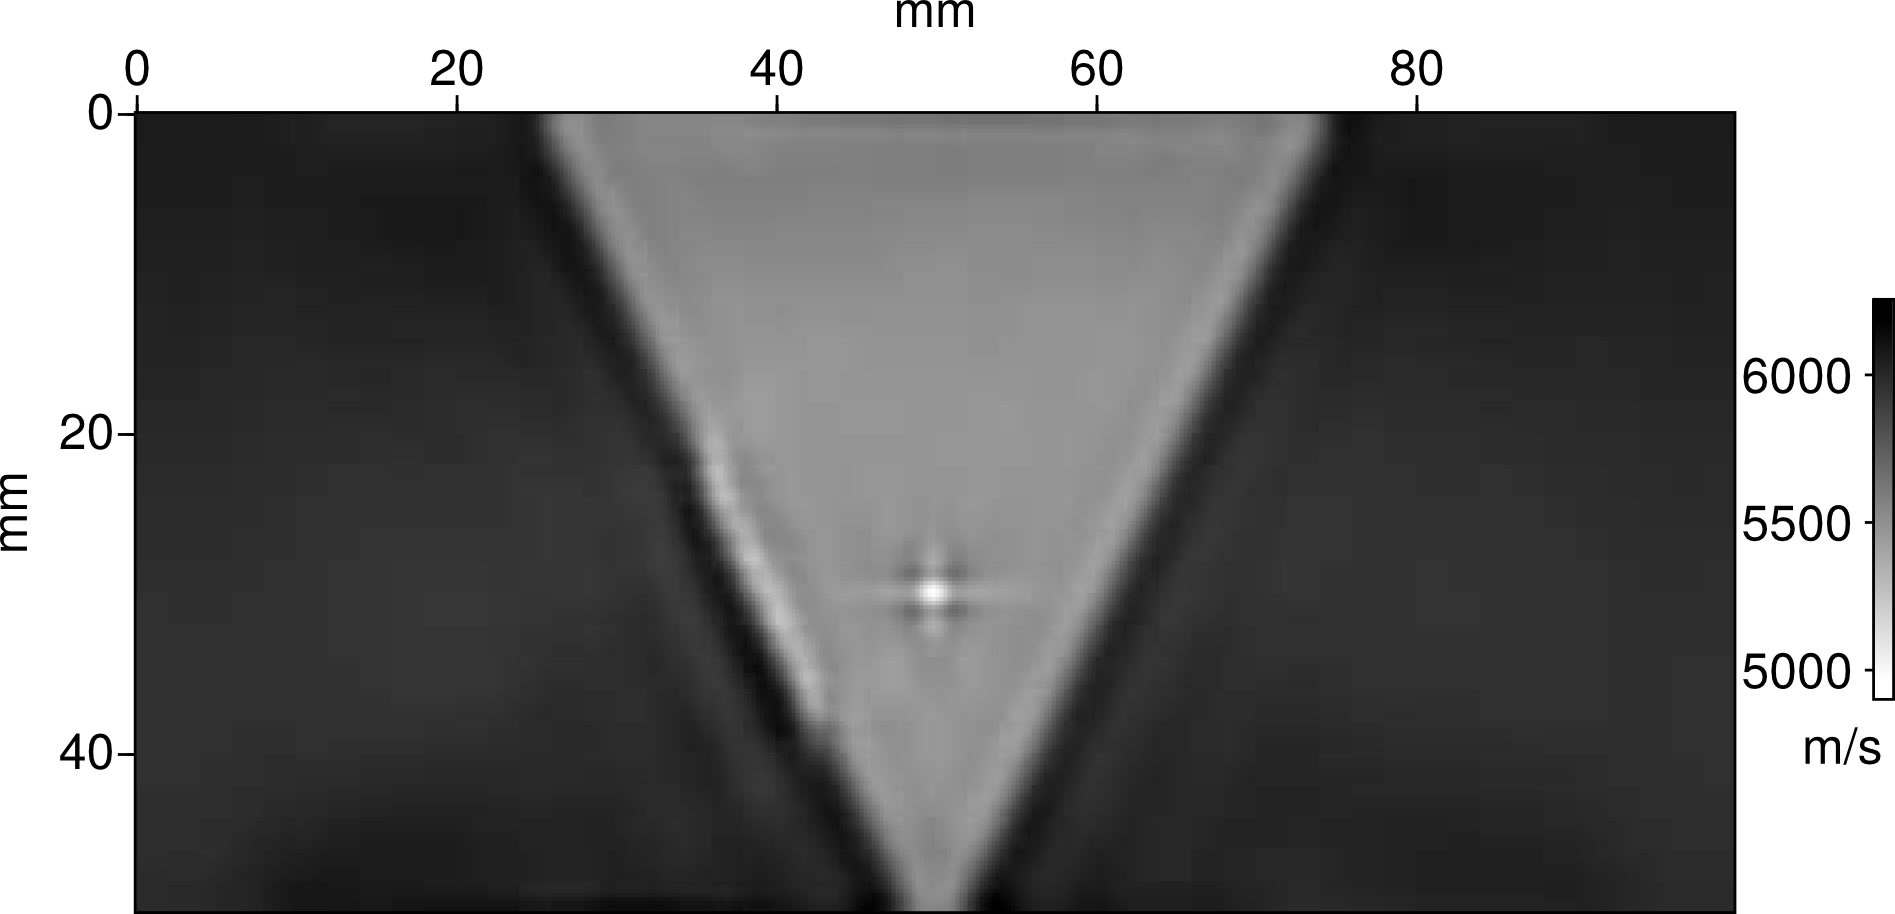
\includegraphics[width=0.7\textwidth]{img/vp_mono_smooth/vp_smooth.png}\\
%		\only<2->{\vspace{0.3cm} Vitesse Reconstruite :\\[0.2cm]}
%		\only<1-1>{\vspace{2.7cm}}
%		\only<2-2>{
%			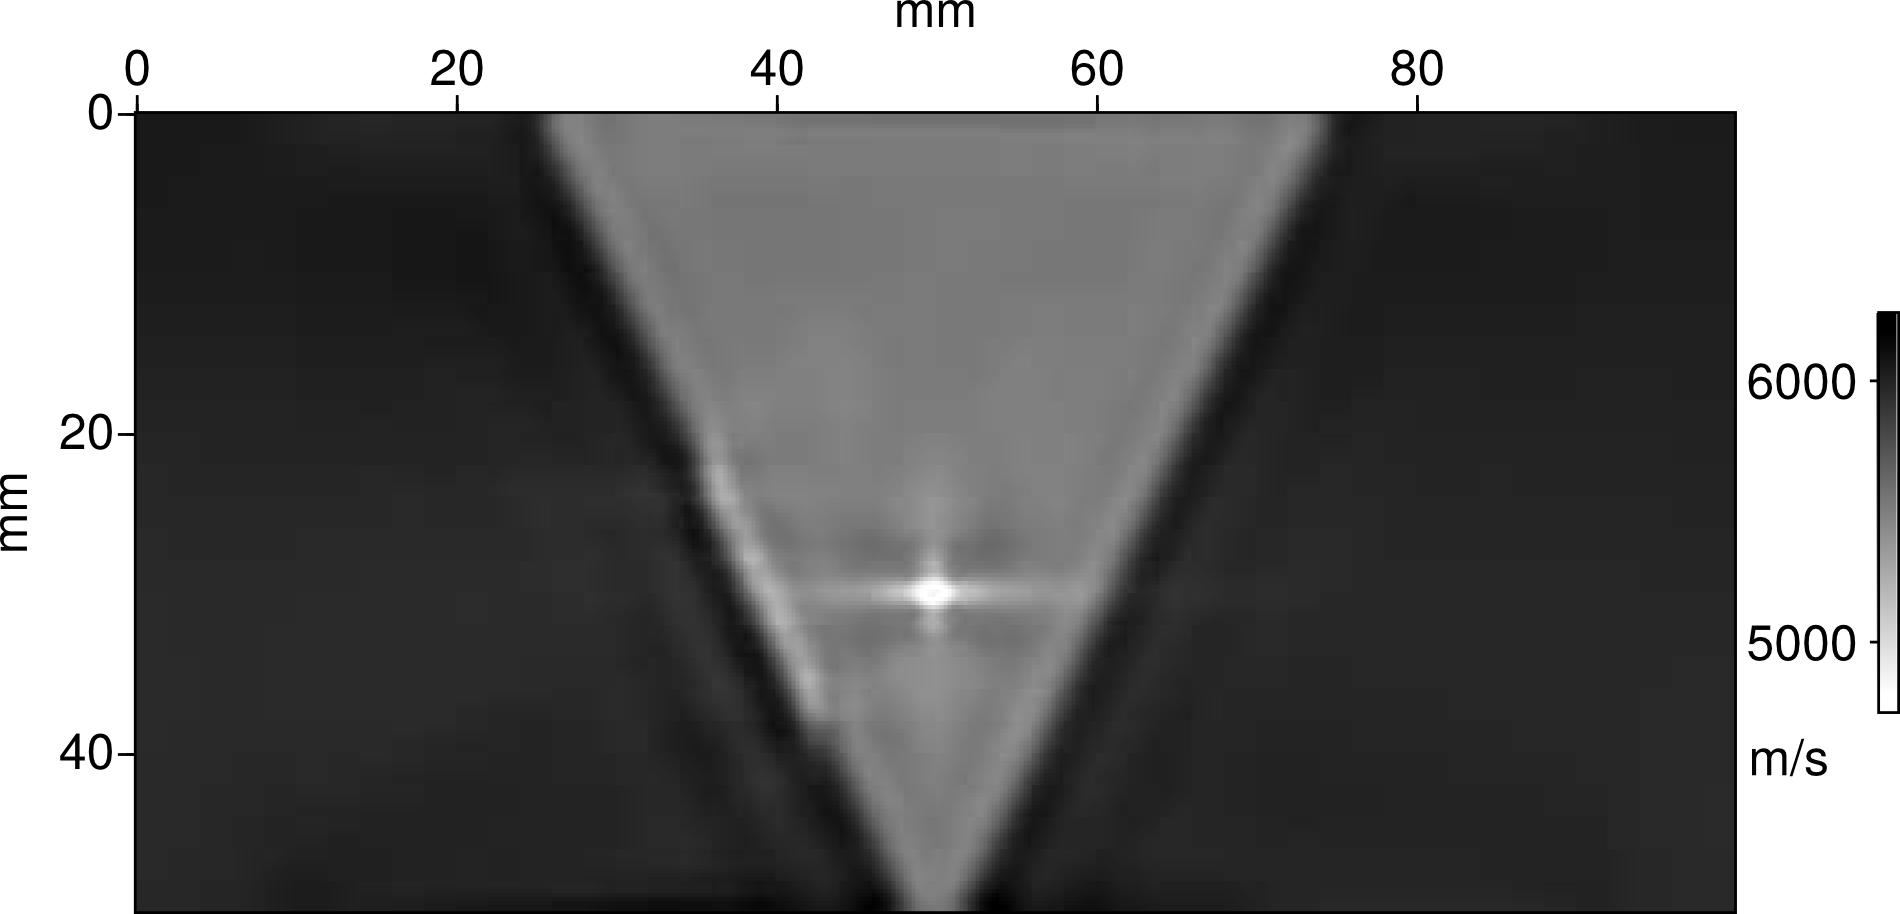
\includegraphics[width=0.7\textwidth]{img/vp_mono_smooth/vp_400k.png}\\		
%		}
%		\only<3-3>{
%			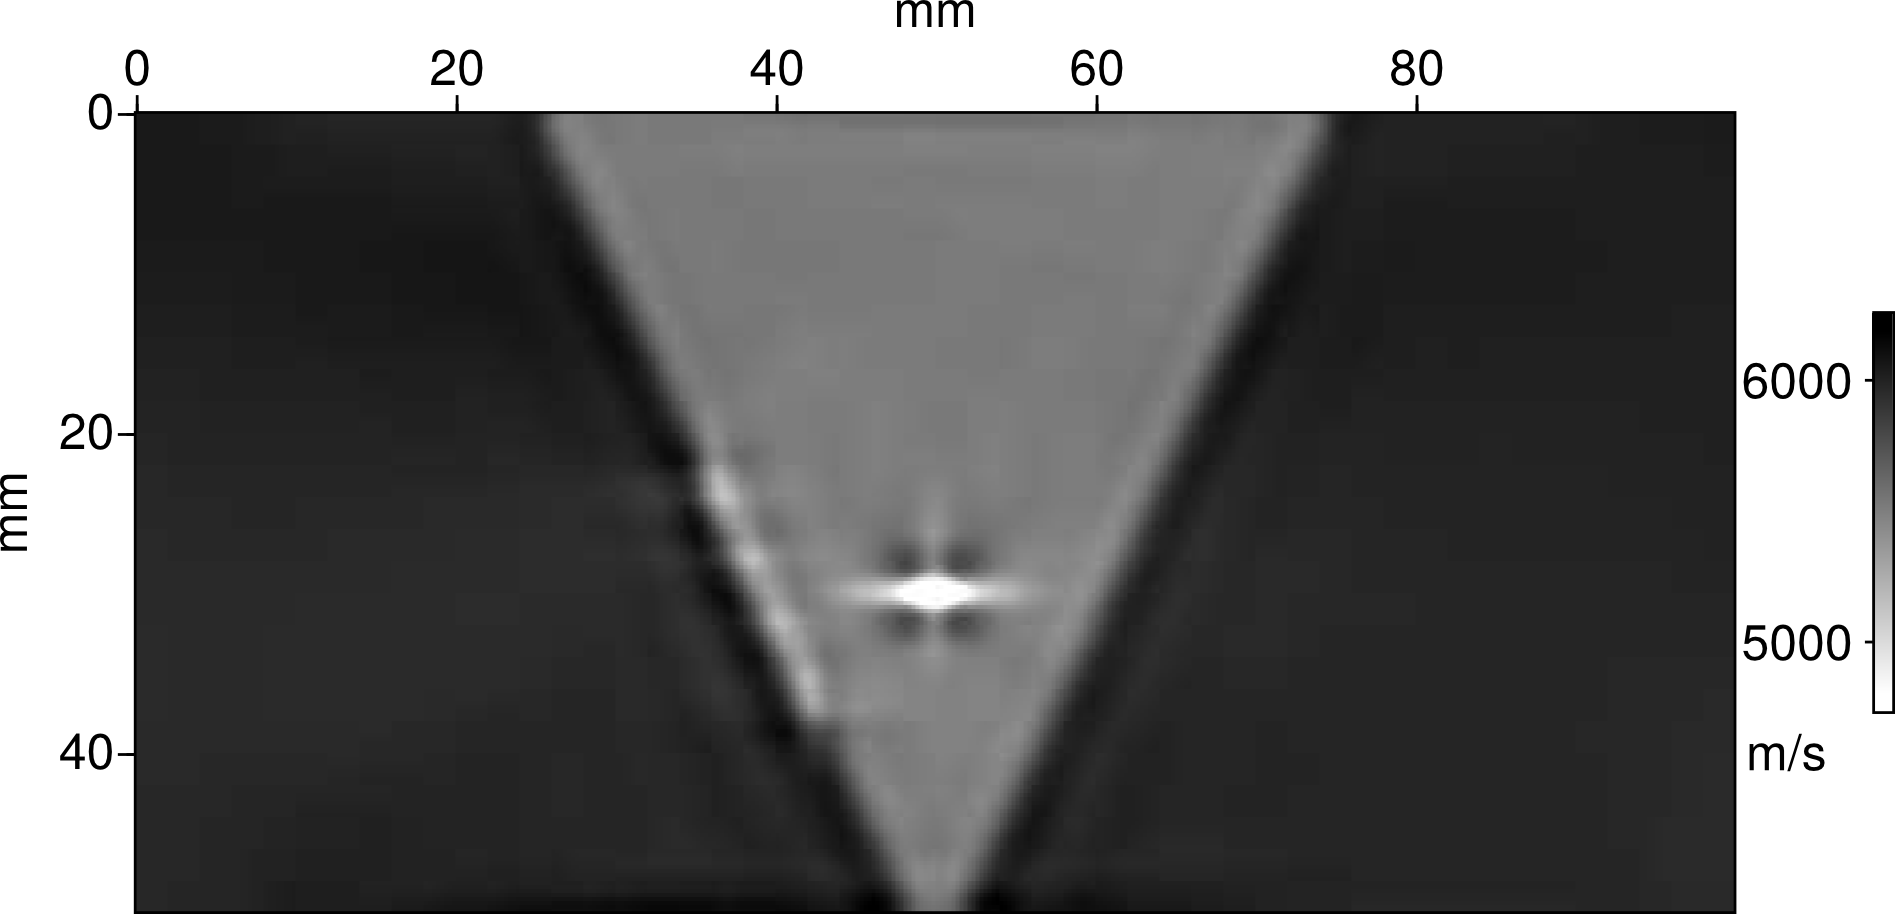
\includegraphics[width=0.7\textwidth]{img/vp_mono_smooth/vp_900k.png}\\		
%		}
%		\only<4-4>{
%			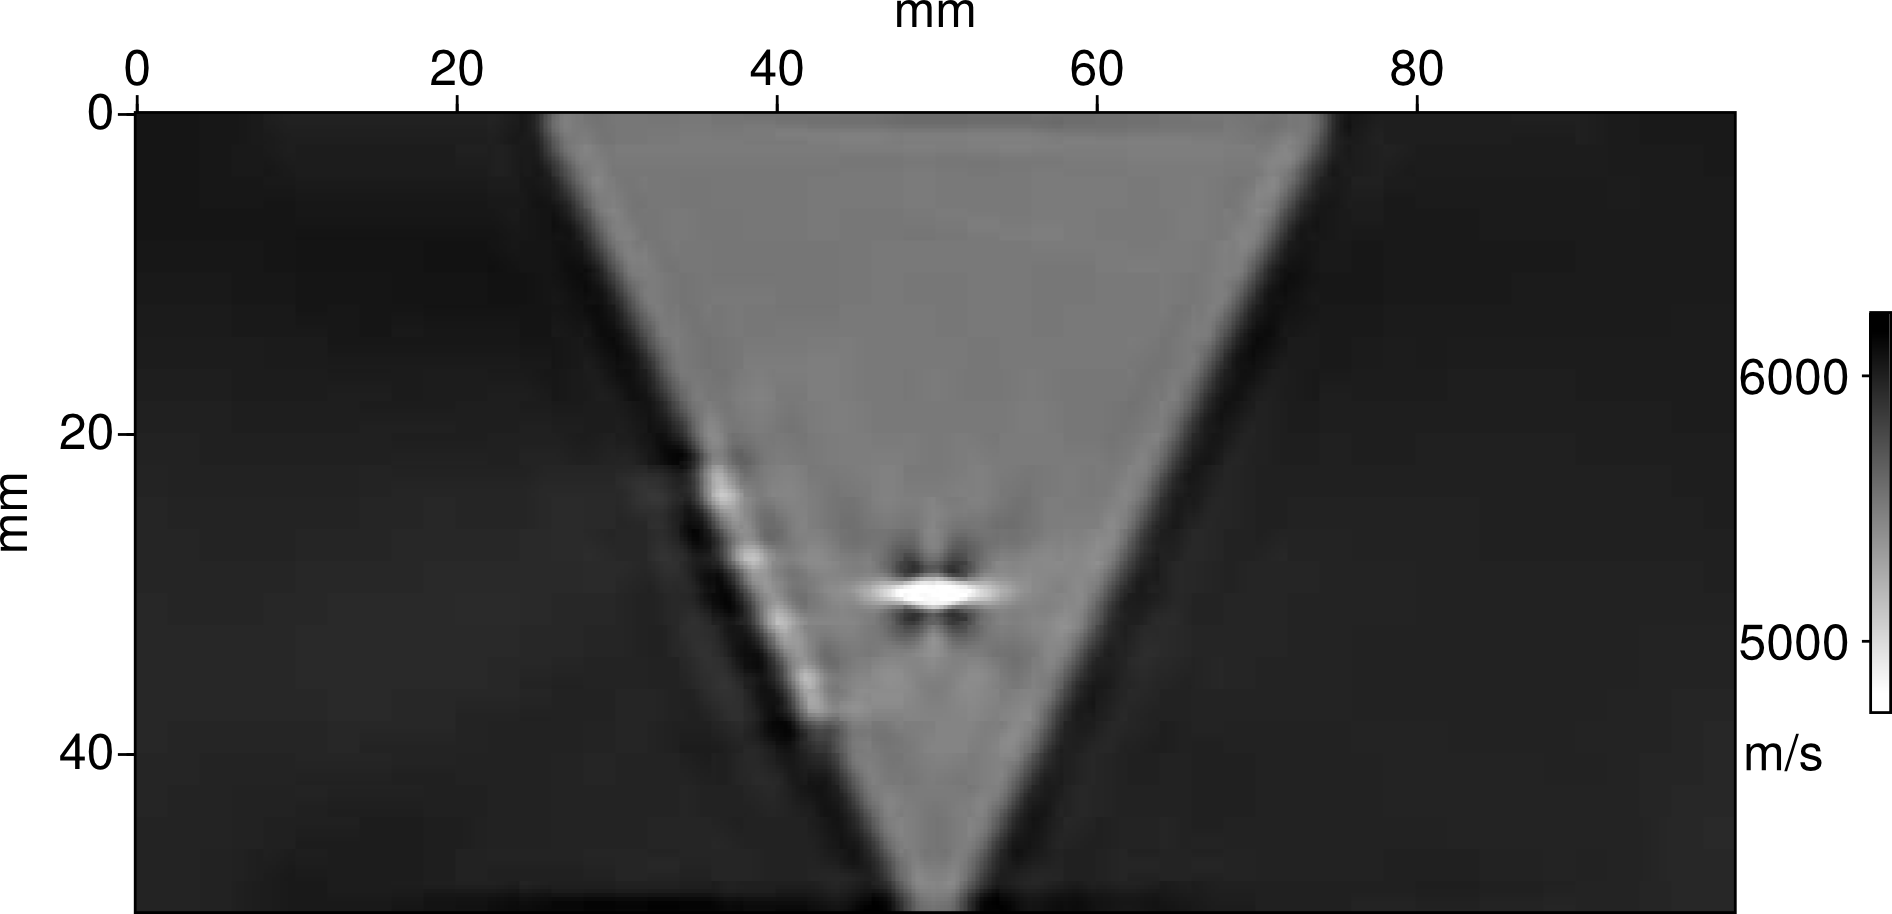
\includegraphics[width=0.7\textwidth]{img/vp_mono_smooth/vp_1300k.png}\\		
%		}
%		\only<5-5>{
%			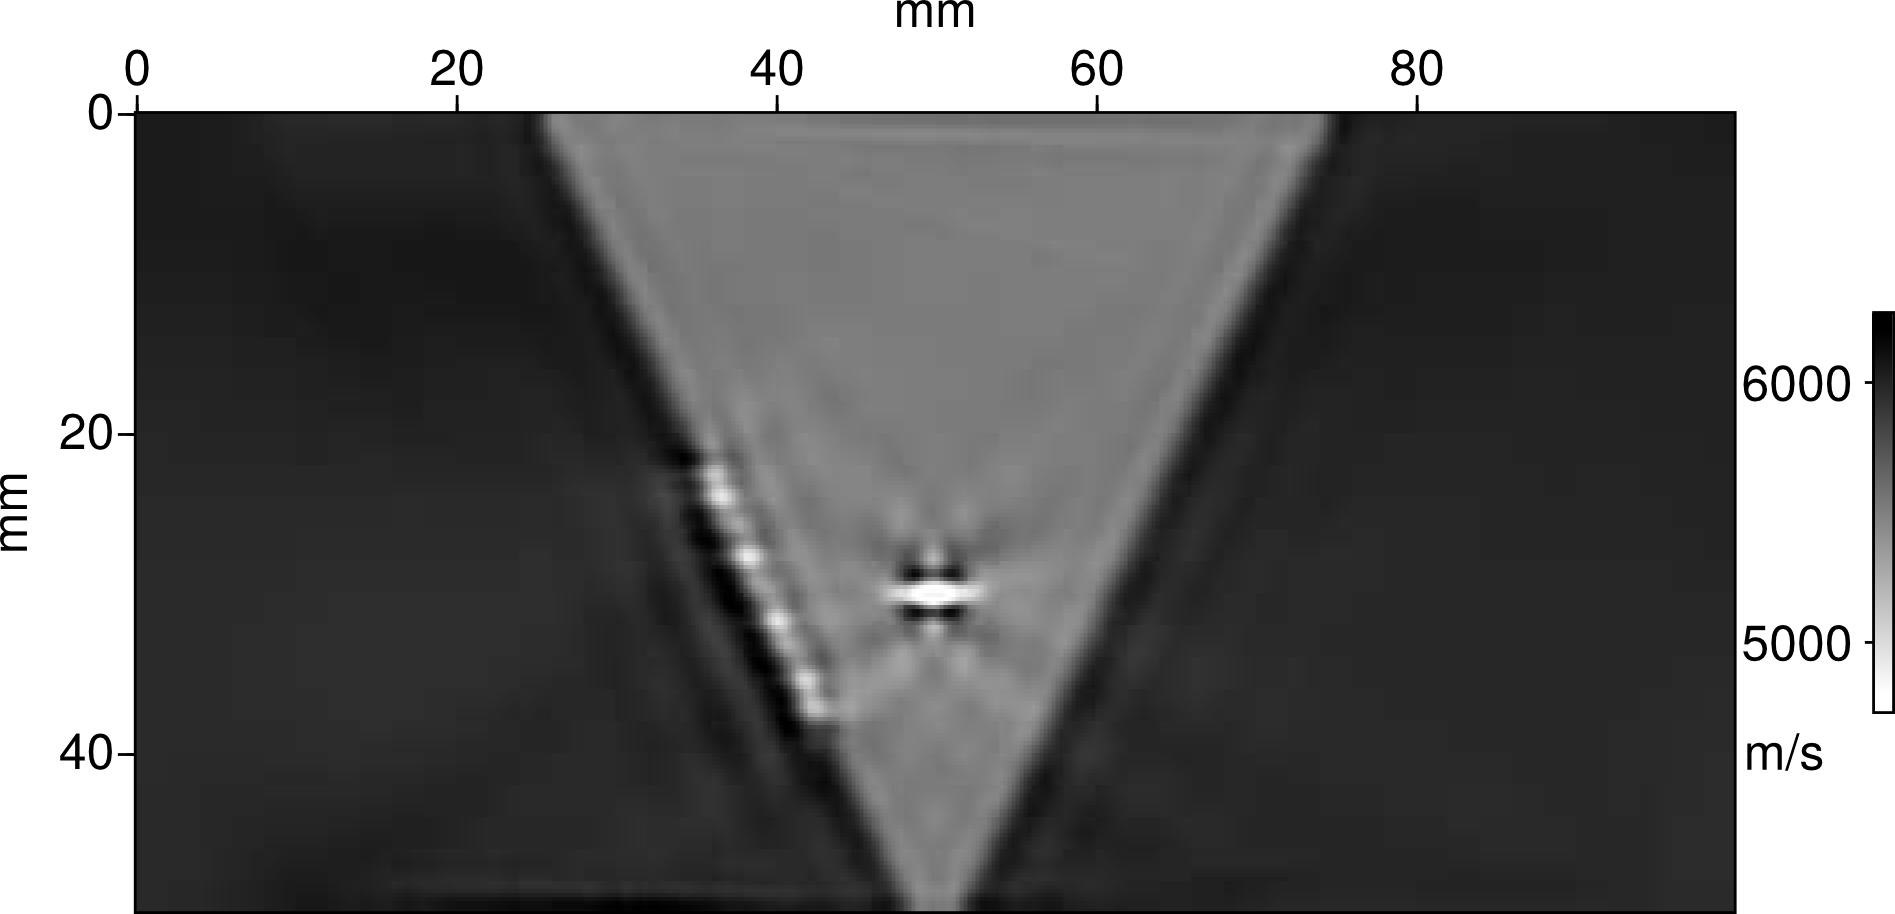
\includegraphics[width=0.7\textwidth]{img/vp_mono_smooth/vp_1950k.png}\\		
%		}
%		\only<6->{
%			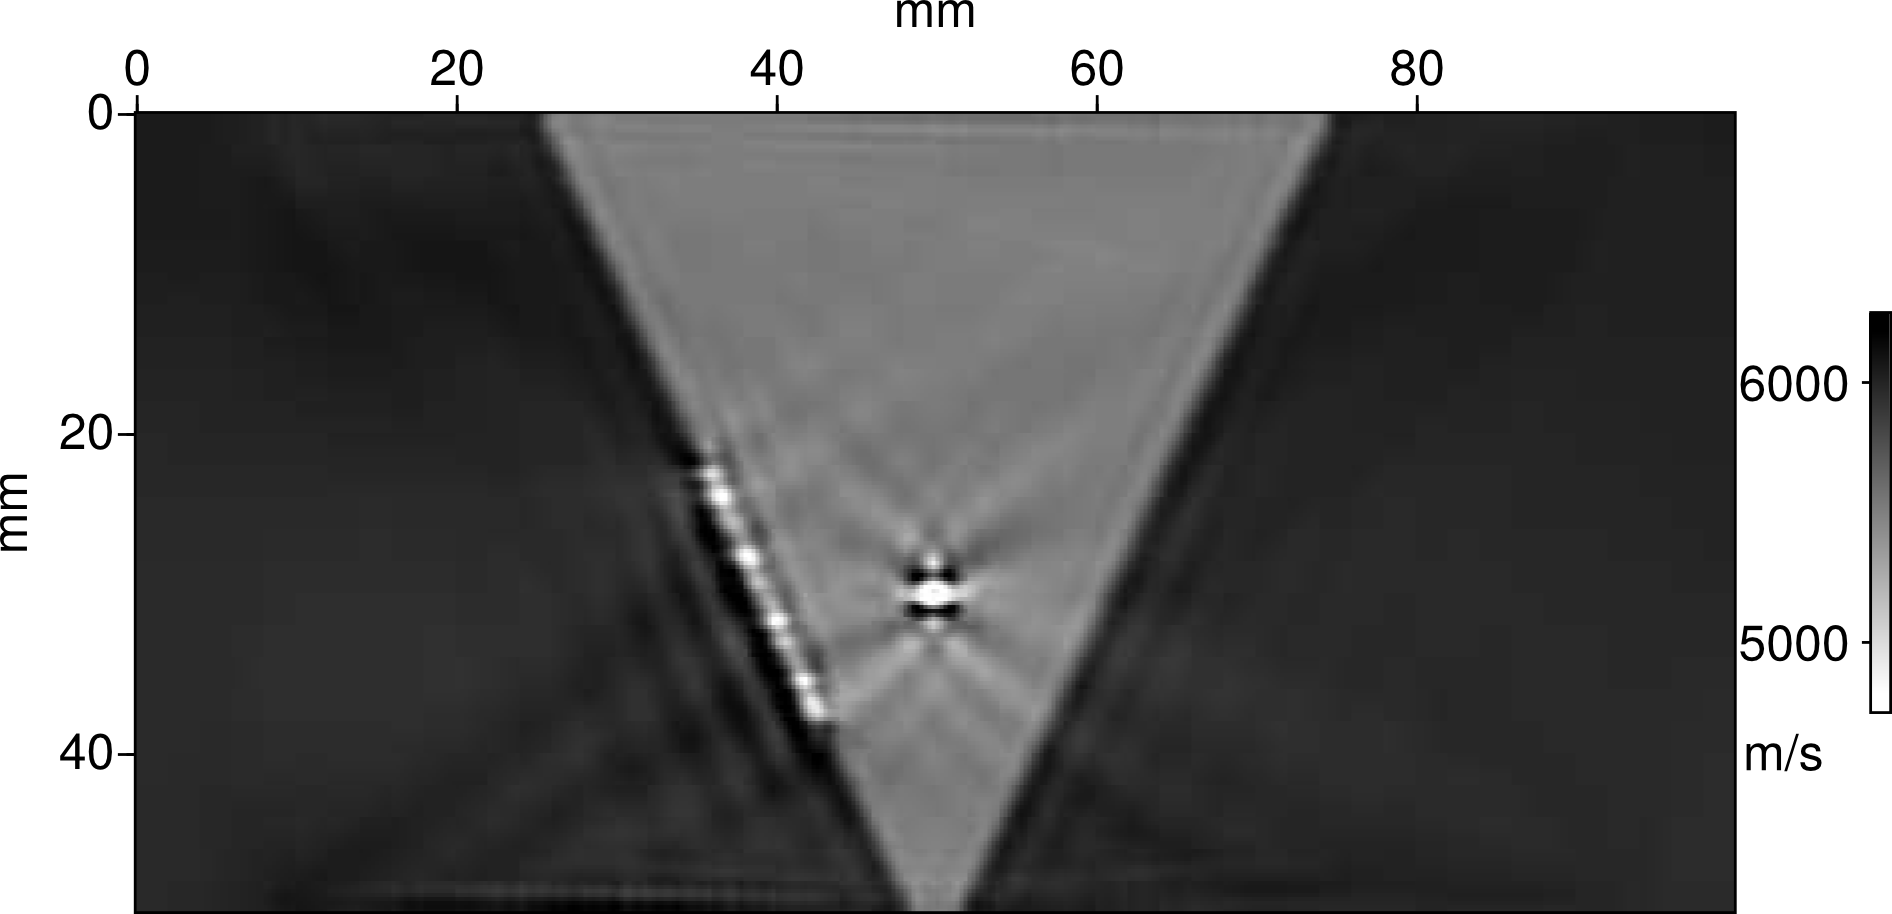
\includegraphics[width=0.7\textwidth]{img/vp_mono_smooth/vp_2900k.png}\\		
%		}
%		
%		
%	\end{columns}
%	\end{adjustwidth}
%	%\vspace{0.3cm} 
%	Vitesse vraie :
%	\begin{figure}
%		\centering
%		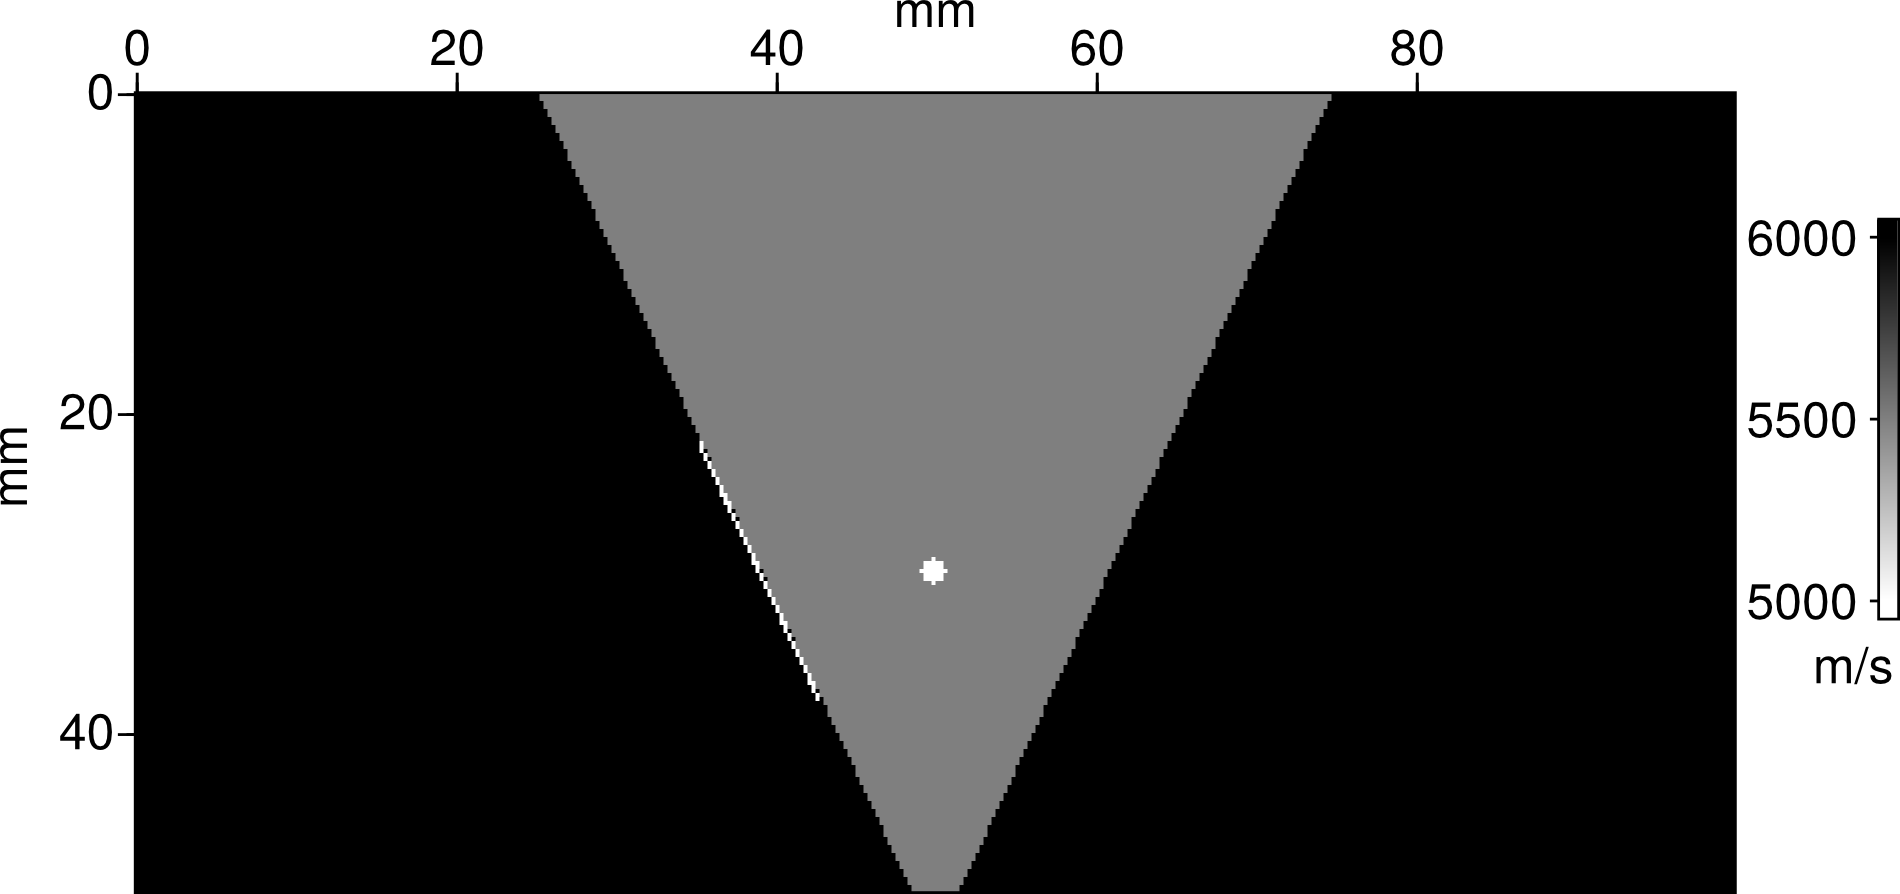
\includegraphics[width=0.35\textwidth]{img/vp_true_sans_acqui.png}\\
%	\end{figure}
%	
%	\begin{picture}(0,0)(0,0)\put(127,120){
%		\only<2-2>{f$\approx$ 400 kHz}
%		\only<3-3>{f$\approx$ 1 MHz~}
%		\only<4-4>{\hspace{-0.1cm}f$\approx$ 1,4 MHz~~}
%		\only<5-5>{\hspace{-0.2cm}f$\approx$ 2 MHz~~~}
%		\only<6-6>{\hspace{-0.2cm}f$\approx$ 3 MHz}
%	}\end{picture}
%\end{small}
%\end{frame}
%
%\subsection*{}
%\begin{frame}{\insertsectionhead~-- Densité}
%\begin{footnotesize}
%
%		\centering
%		\begin{columns}
%			\column{0.5\textwidth}
%			\raggedleft
%			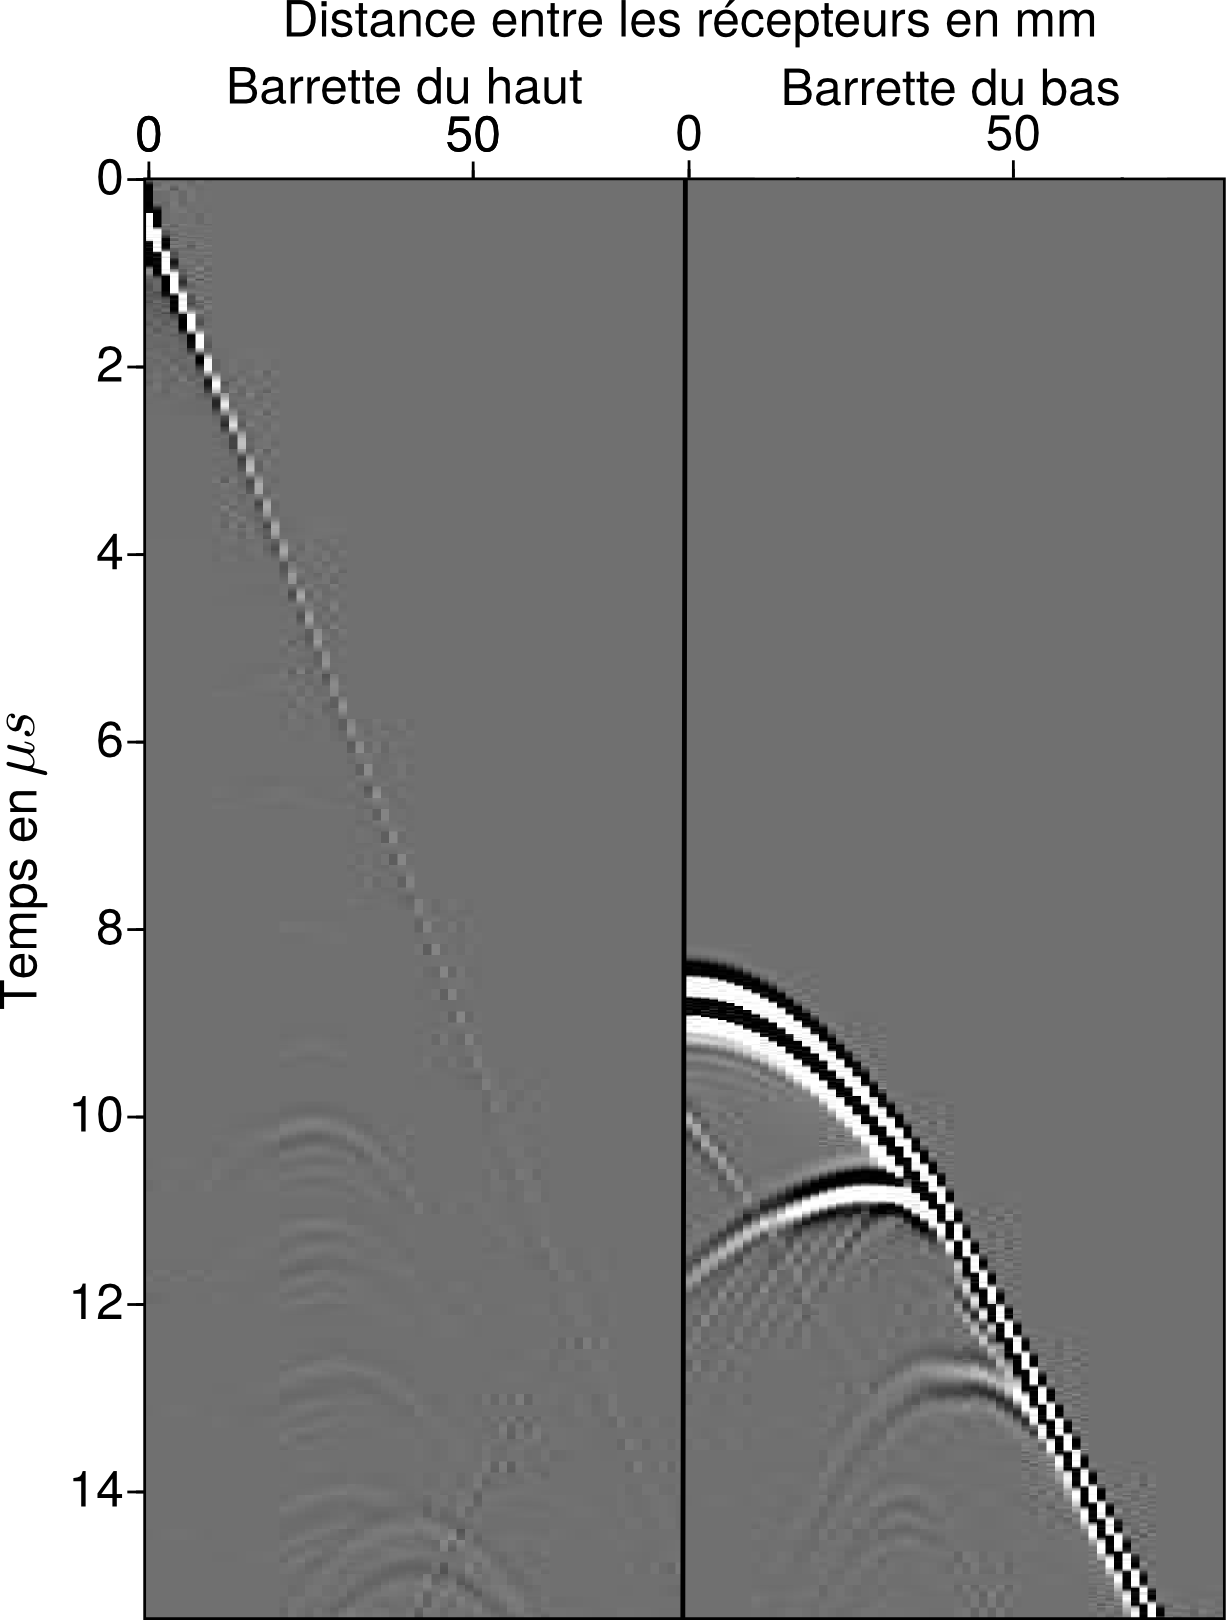
\includegraphics[width=3cm]{img/rho_mono/data_rho_uni.png}\\
%			Signaux issus de $\rho$ homogène\hspace{-0.5cm}
%			\column{0.5\textwidth}
%			\raggedright
%			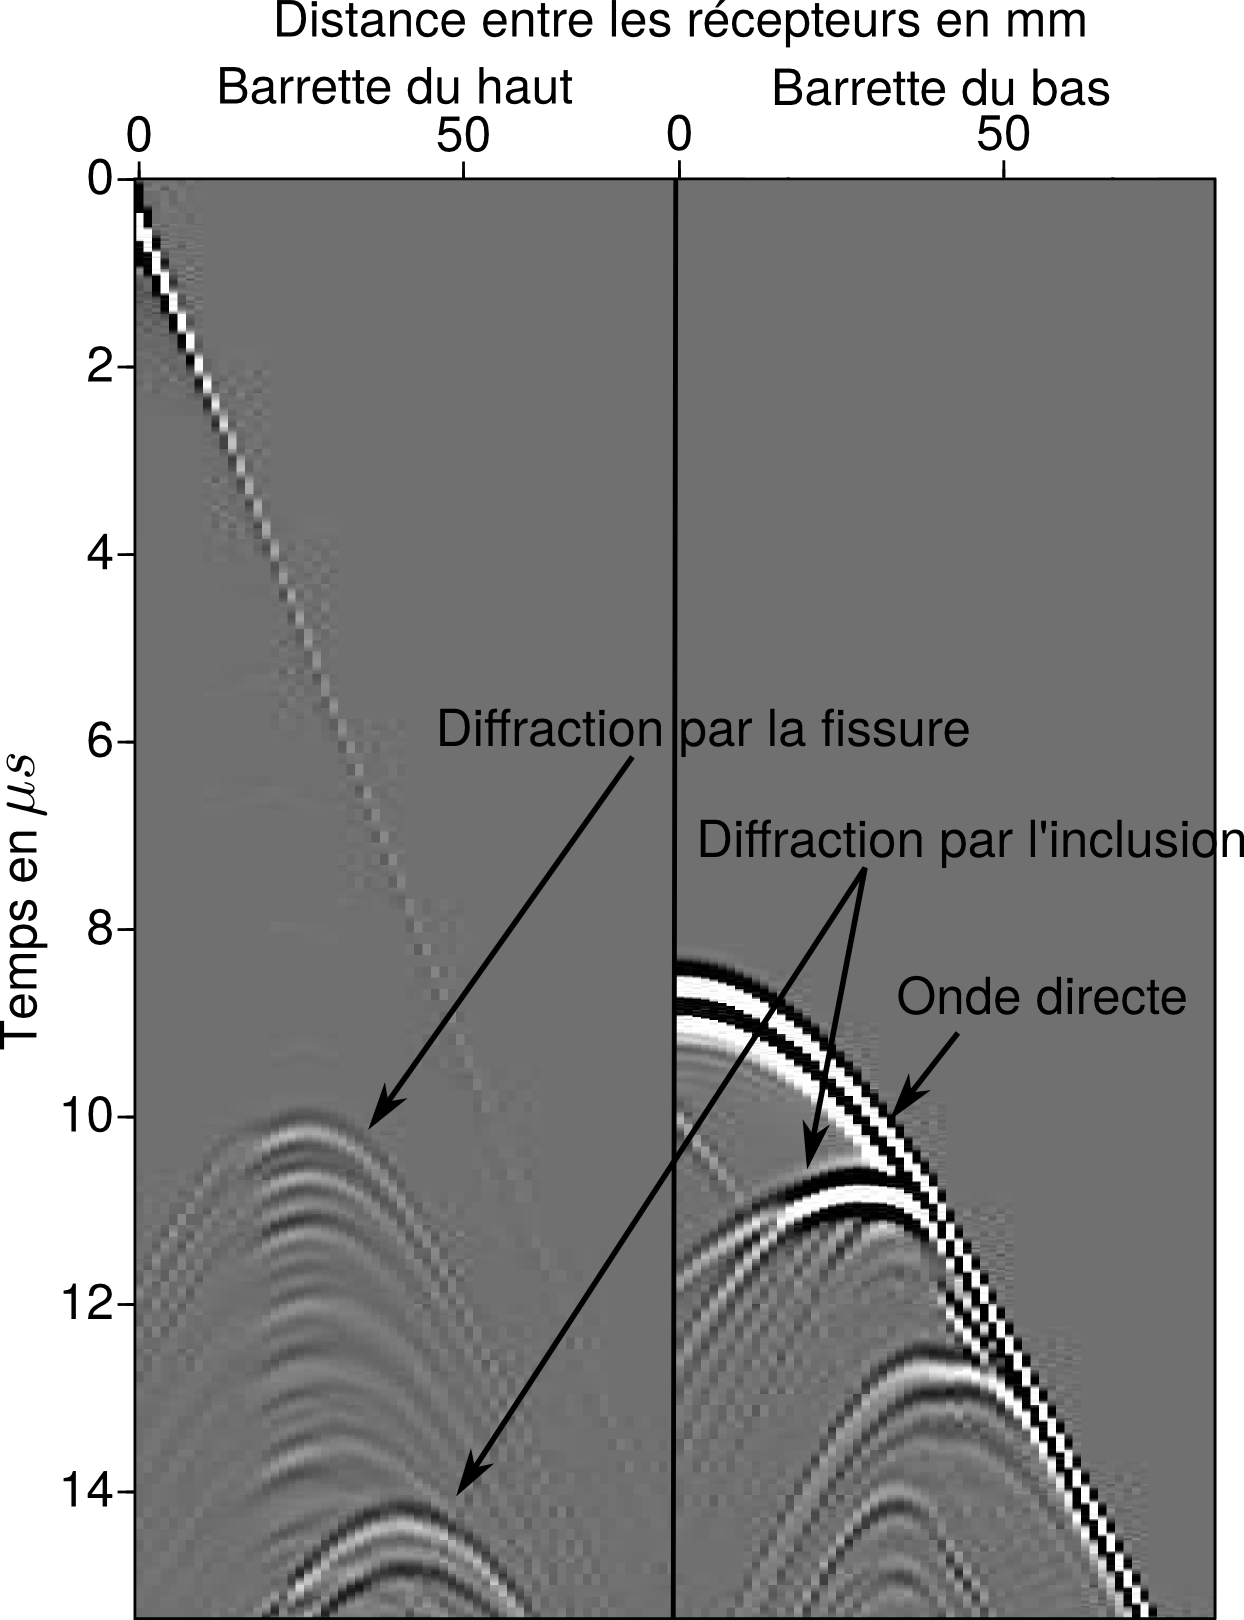
\includegraphics[width=3cm]{img/rho_mono/data_rho_vrai.png}\\
%			~~~Signaux issus de $\rho$ vraie
%		\end{columns}		
%		\vfill
%		
%		\begin{columns}
%			\column{0.35\textwidth}	
%			\centering
%			Modèle initial de vitesse : \\[0.2cm]
%			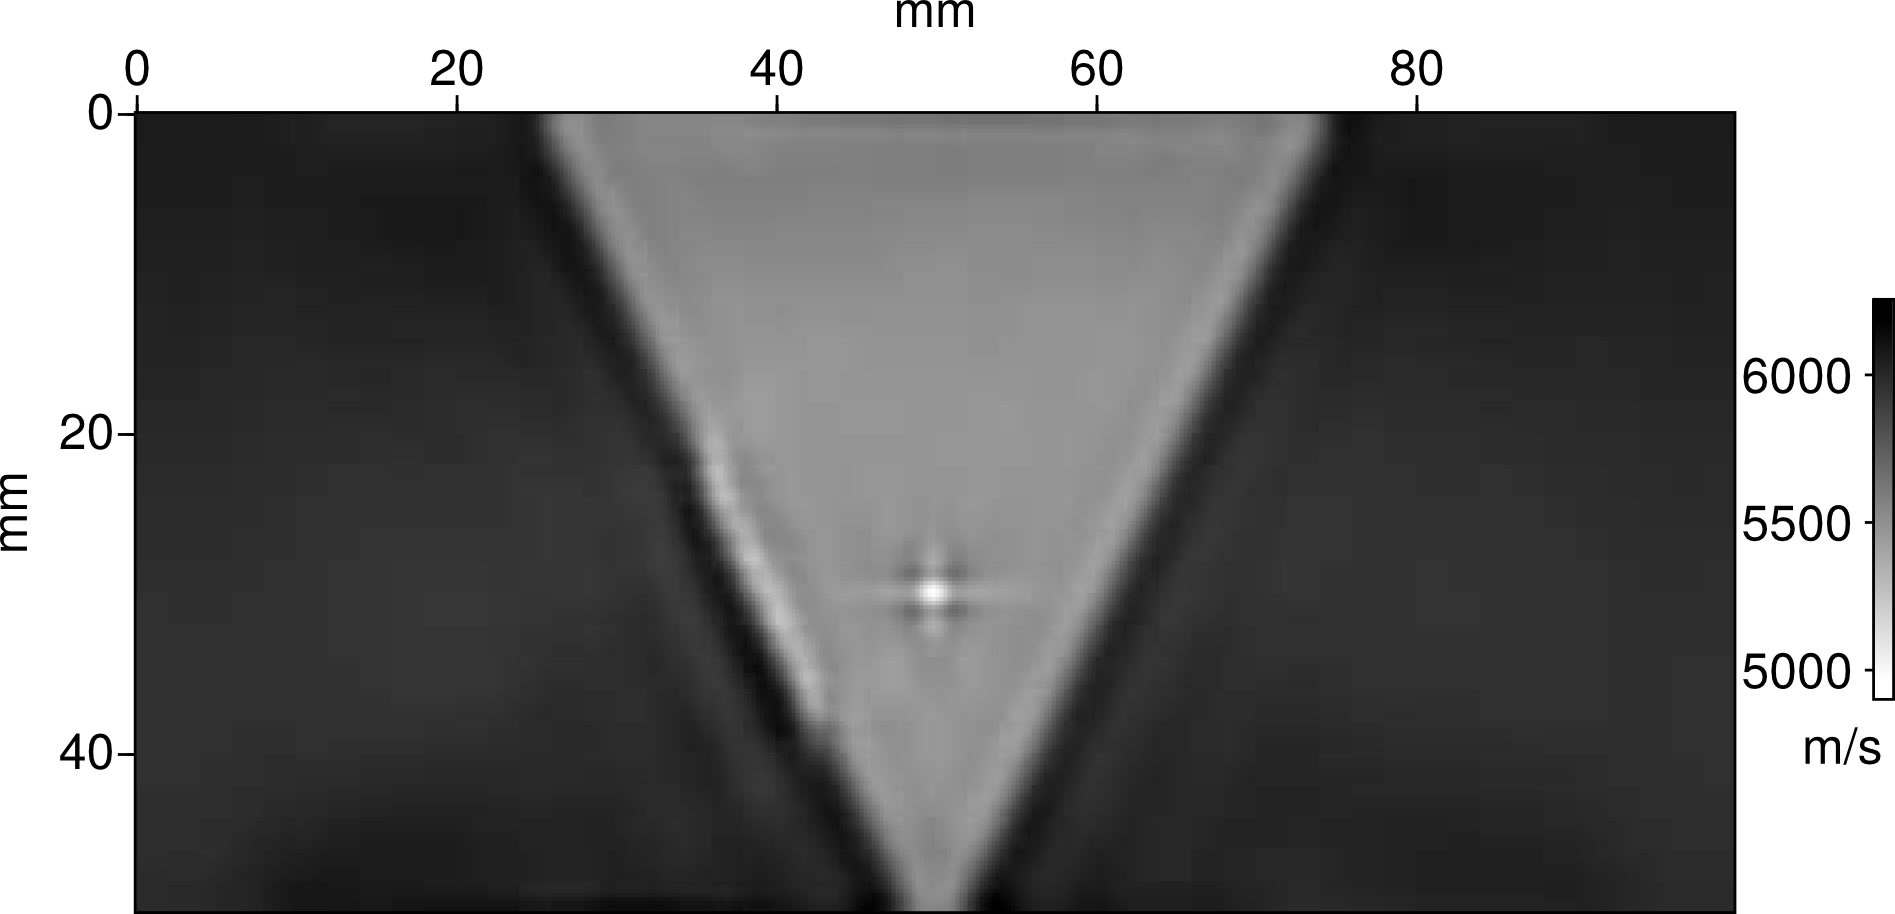
\includegraphics[width=\textwidth]{img/vp_mono_smooth/vp_smooth.png}\\
%			
%			\column{0.35\textwidth}
%			\centering
%			Masse volumique reconstruite :  \\[0.2cm]
%			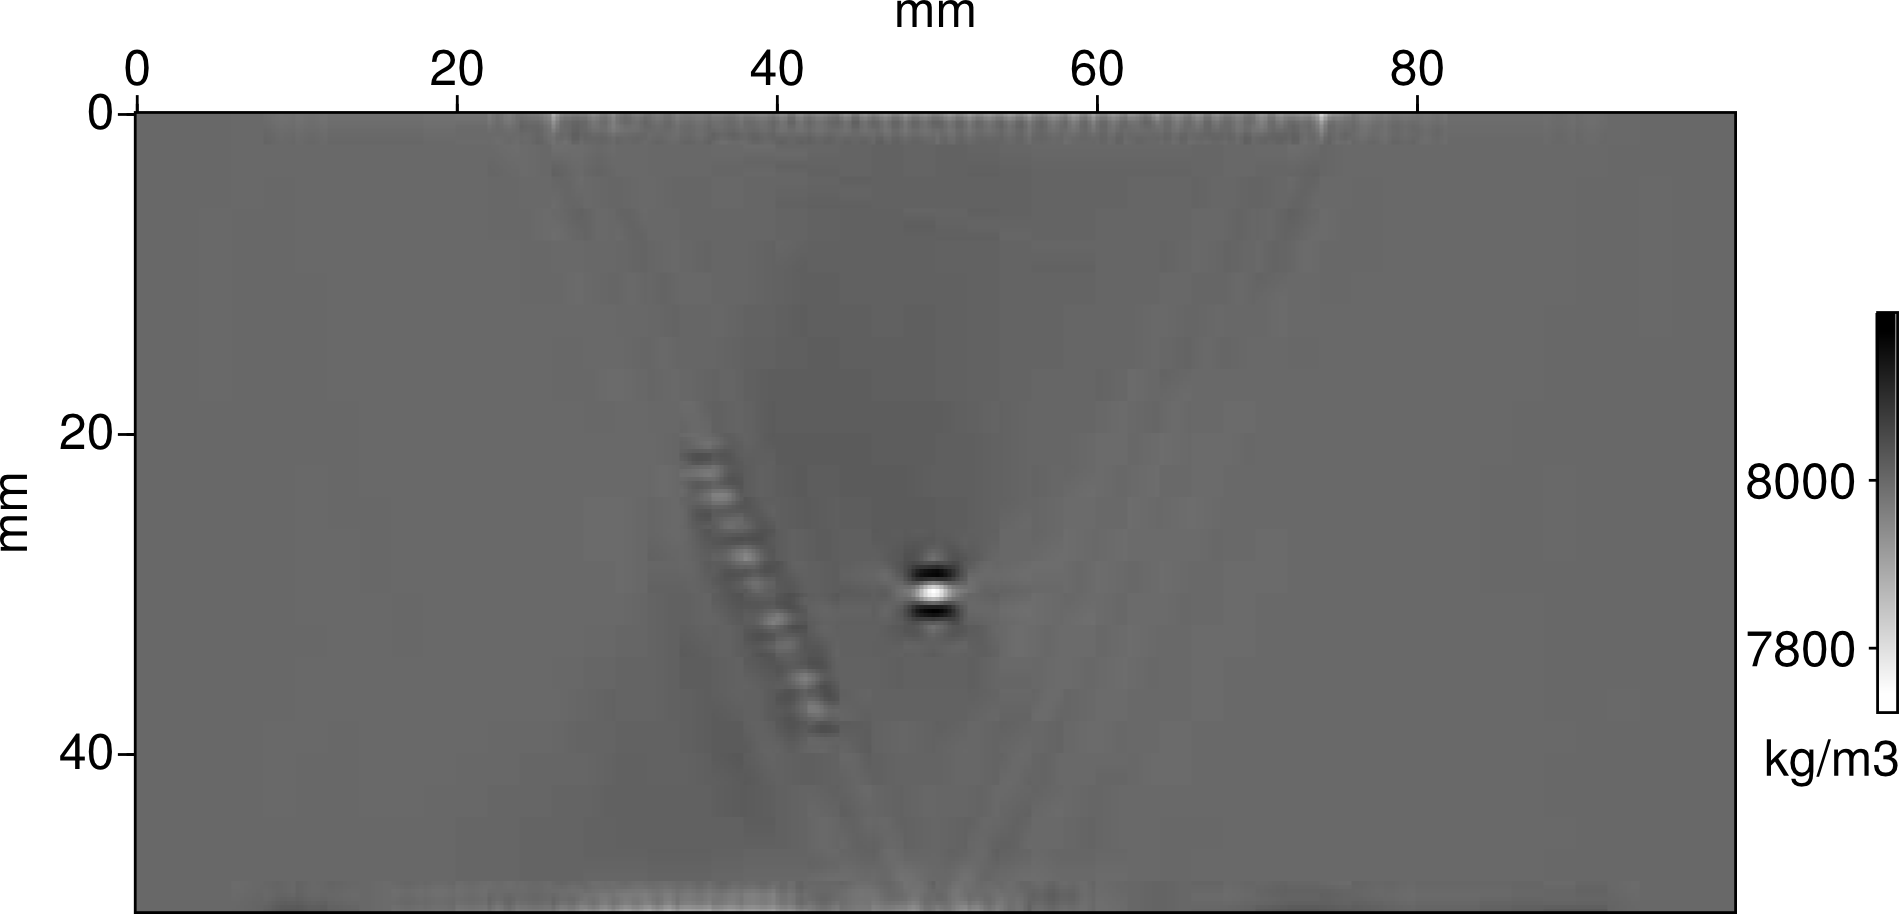
\includegraphics[width=\textwidth]{img/rho_mono/rho_mono.png}\\
%	
%			\column{0.35\textwidth}
%			\centering
%			Masse volumique vraie : \\[0.2cm]
%			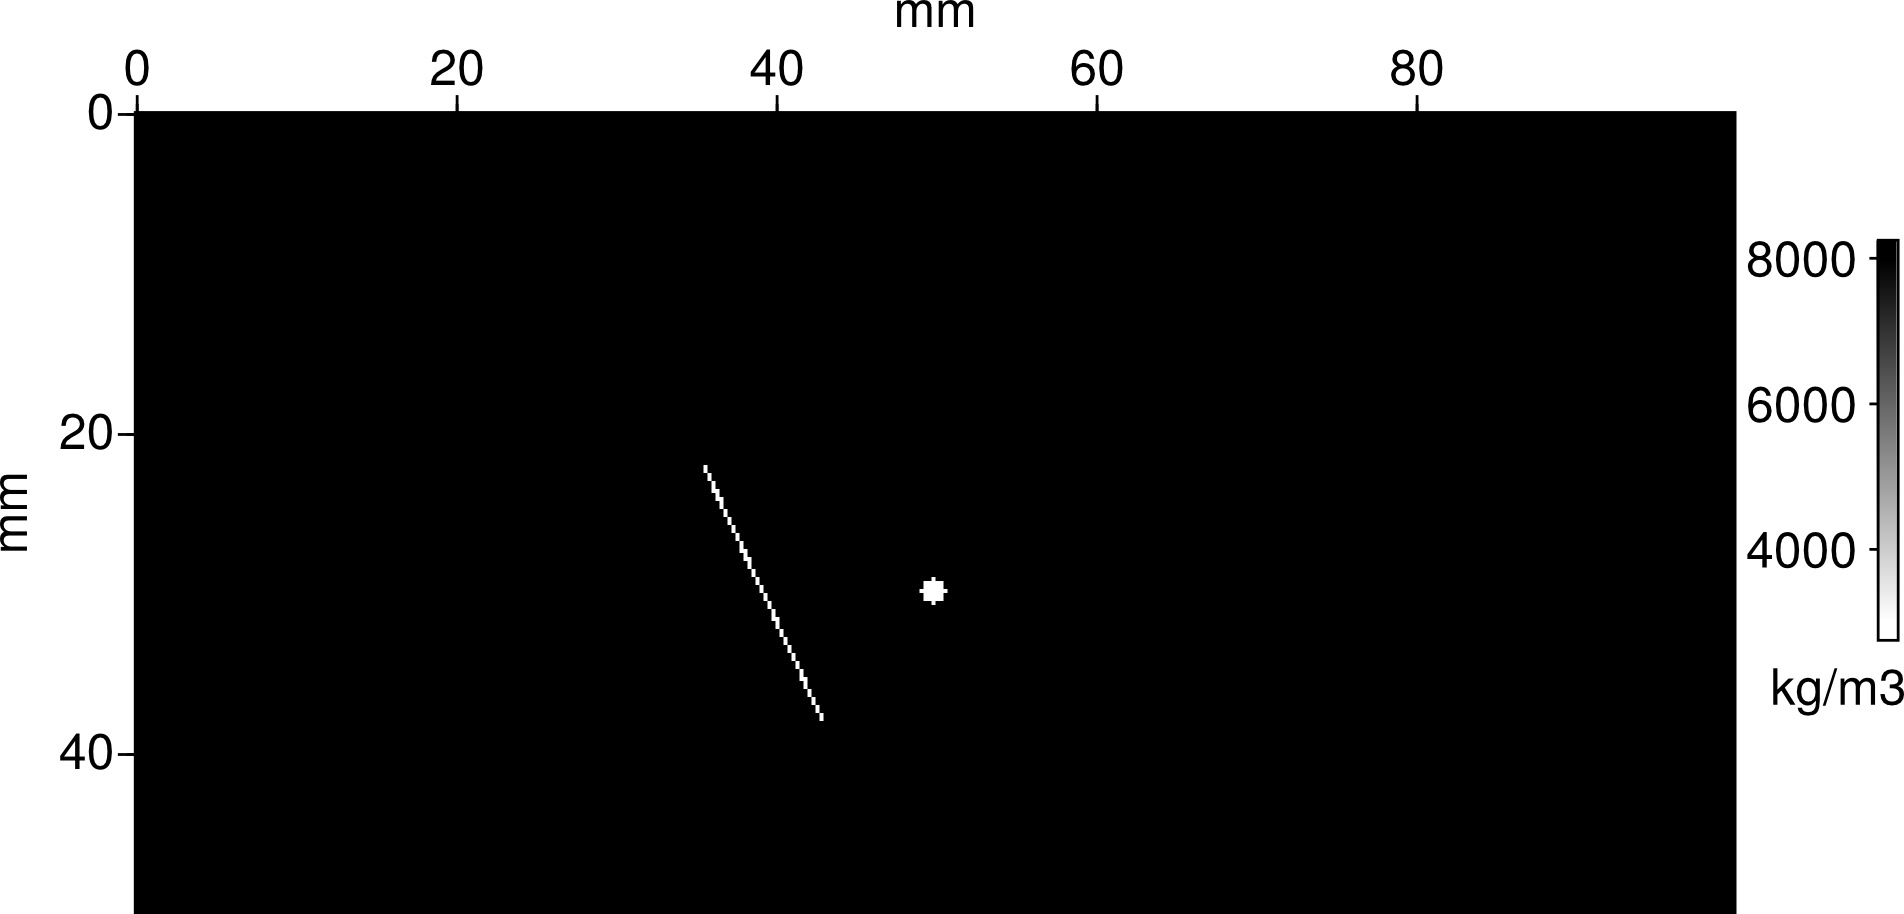
\includegraphics[width=\textwidth]{img/rho_true.png}
%		\end{columns}
%
%\end{footnotesize}		
%\end{frame}
%
%
%\subsection{Inversion multiparamètre}
%\begin{frame}{Isotropic case}
%\begin{small}
%	\centering
%	Vitesse initiale :
%	\begin{figure}
%		\centering
%		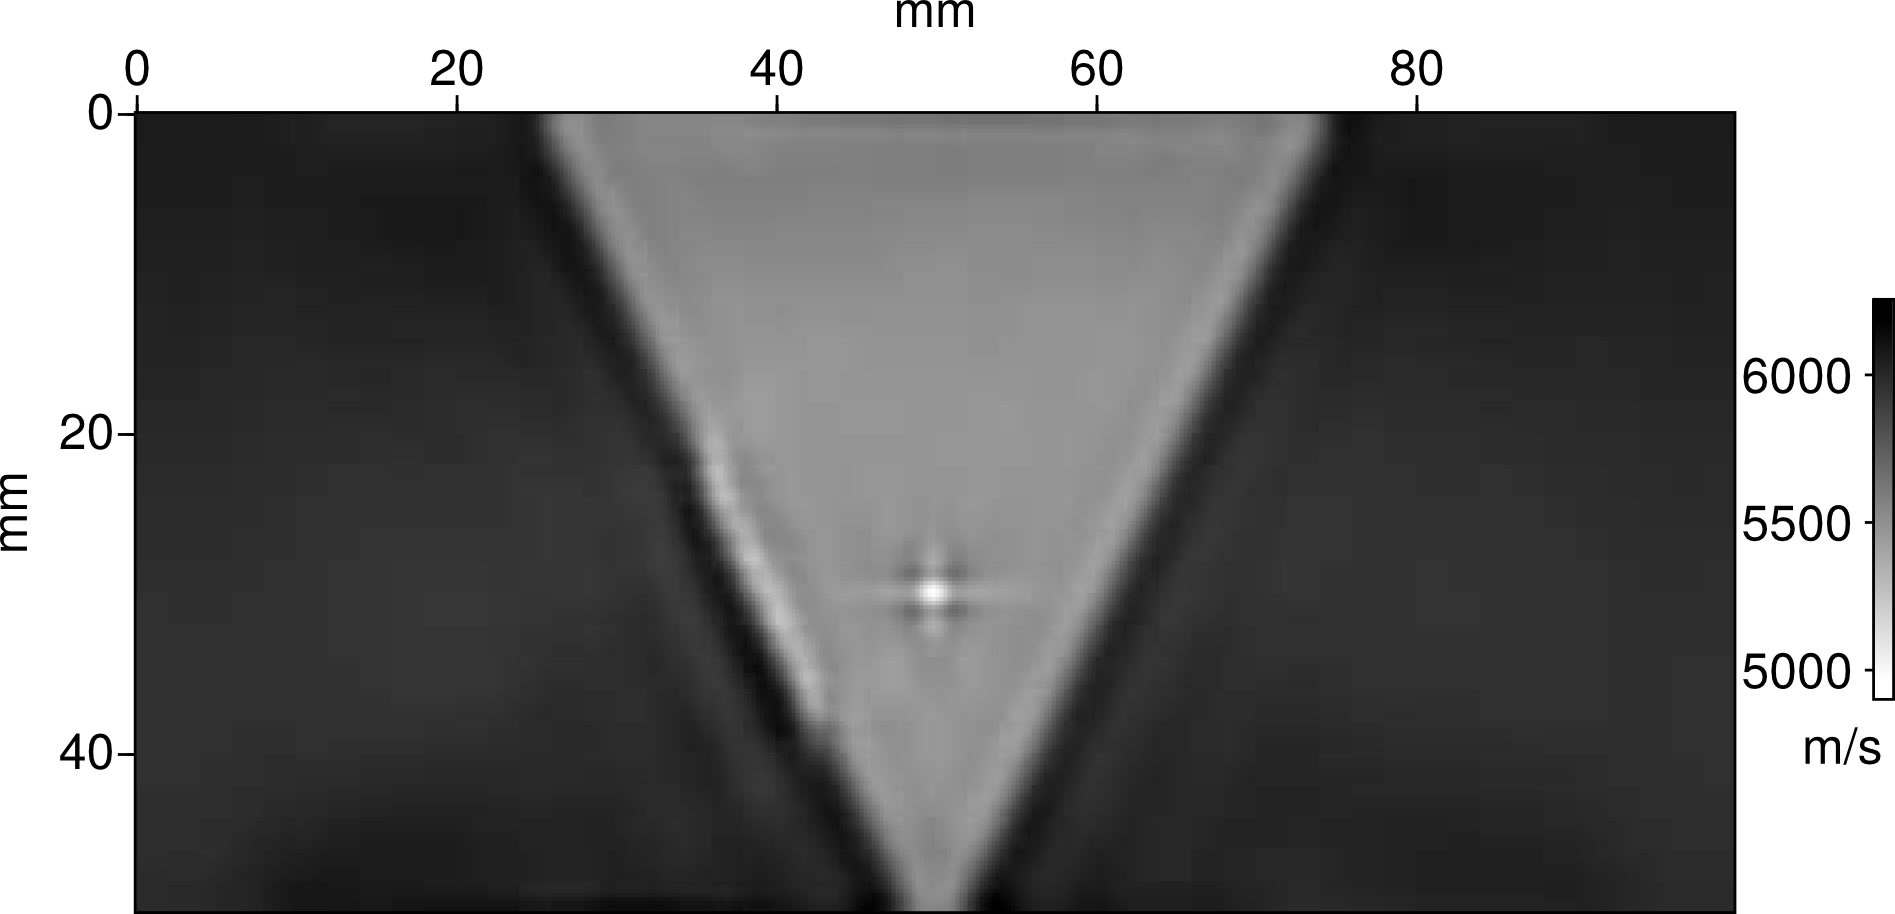
\includegraphics[width=0.35\textwidth]{img/vp_mono_smooth/vp_smooth.png}\\
%	\end{figure}
%	
%	\begin{columns}
%		\column{0.5\textwidth}
%		\centering
%		Vitesse reconstruite :\\[0.2cm]
%		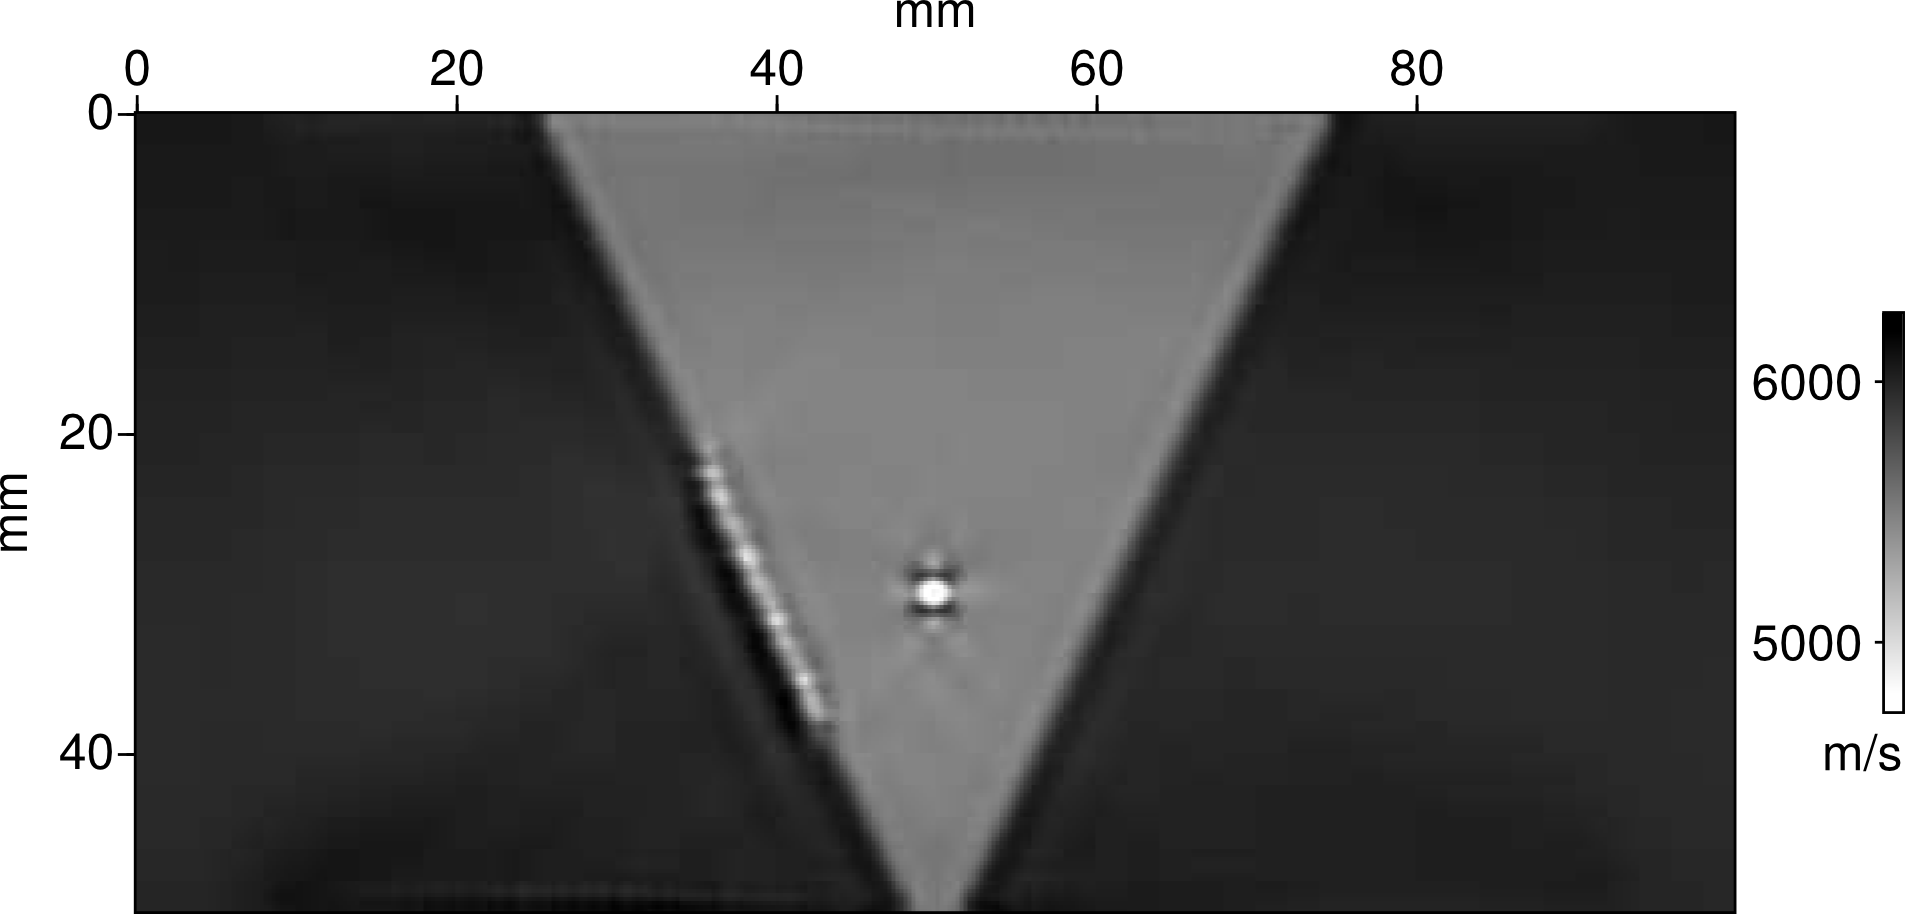
\includegraphics[width=0.7\textwidth]{img/multi/vp_multi_6000k.png}	\\
%		
%		Vitesse vraie : \\[0.2cm]
%		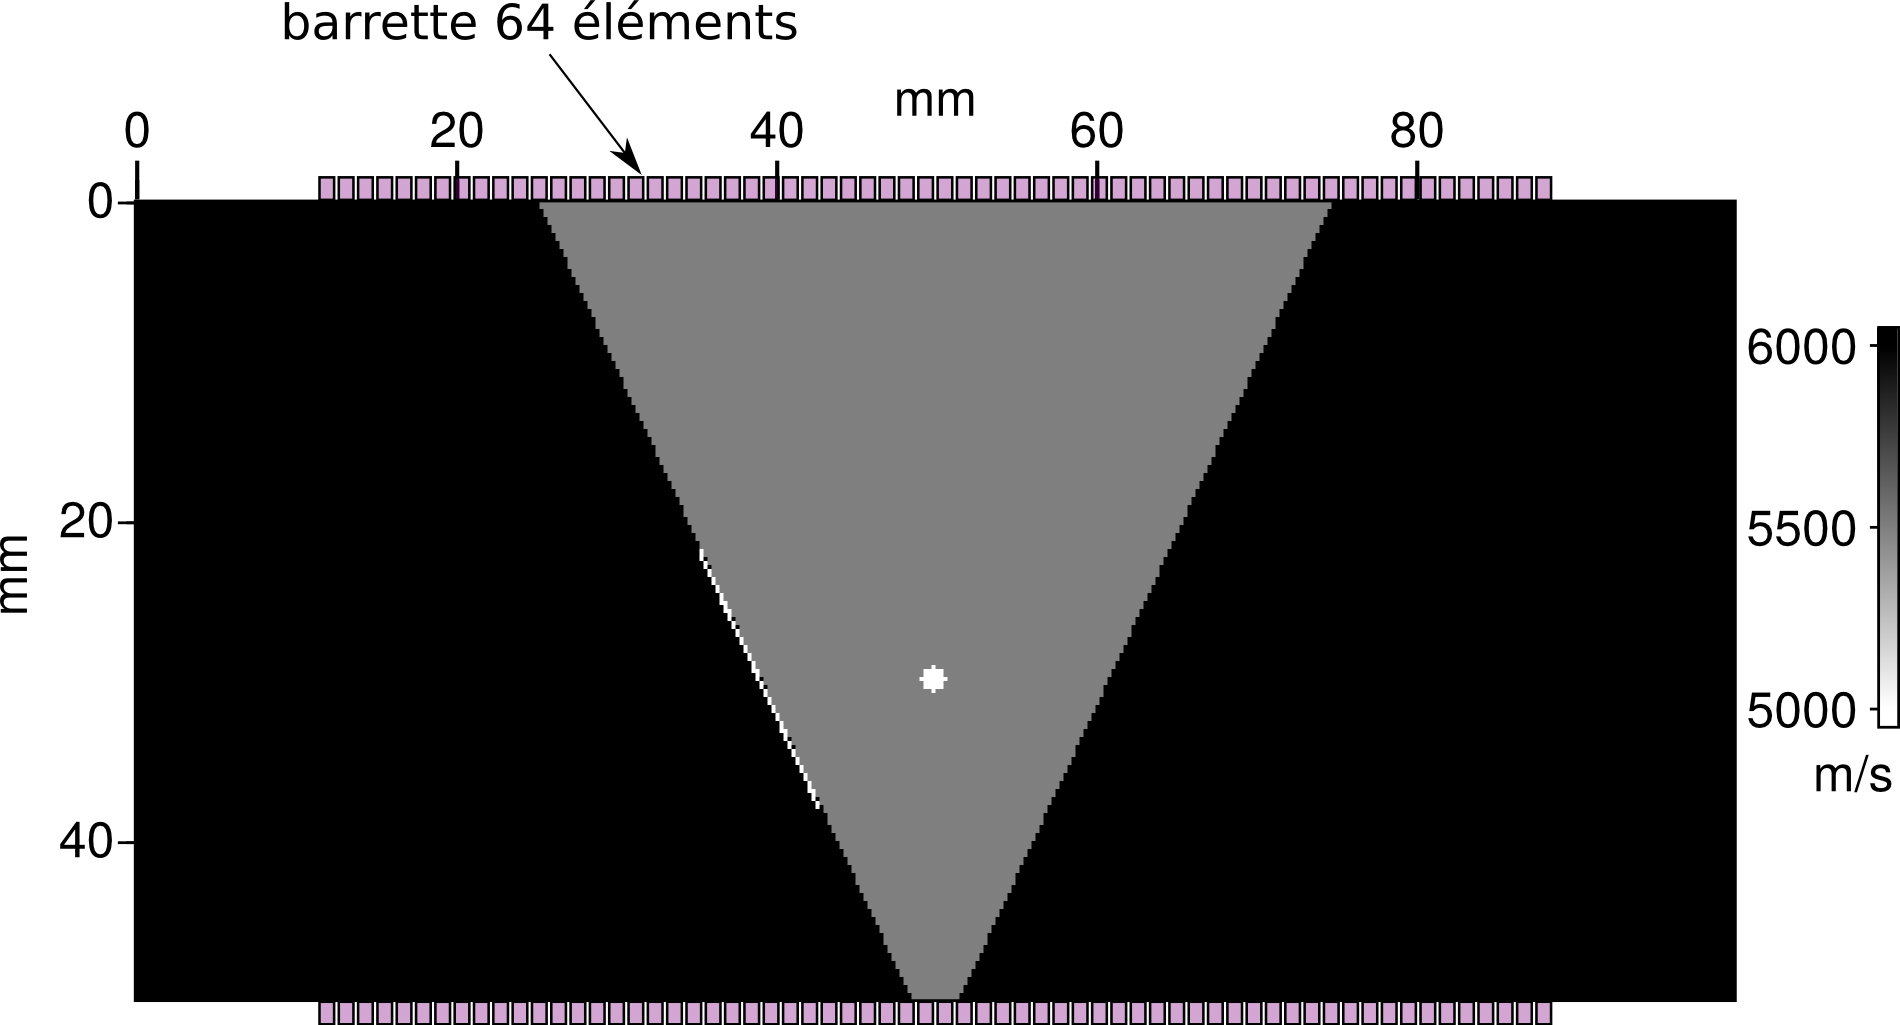
\includegraphics[width=0.7\textwidth]{img/vp_true.png}
%		\column{0.5\textwidth}
%		\centering
%		Masse volumique reconstruite :\\[0.2cm]
%		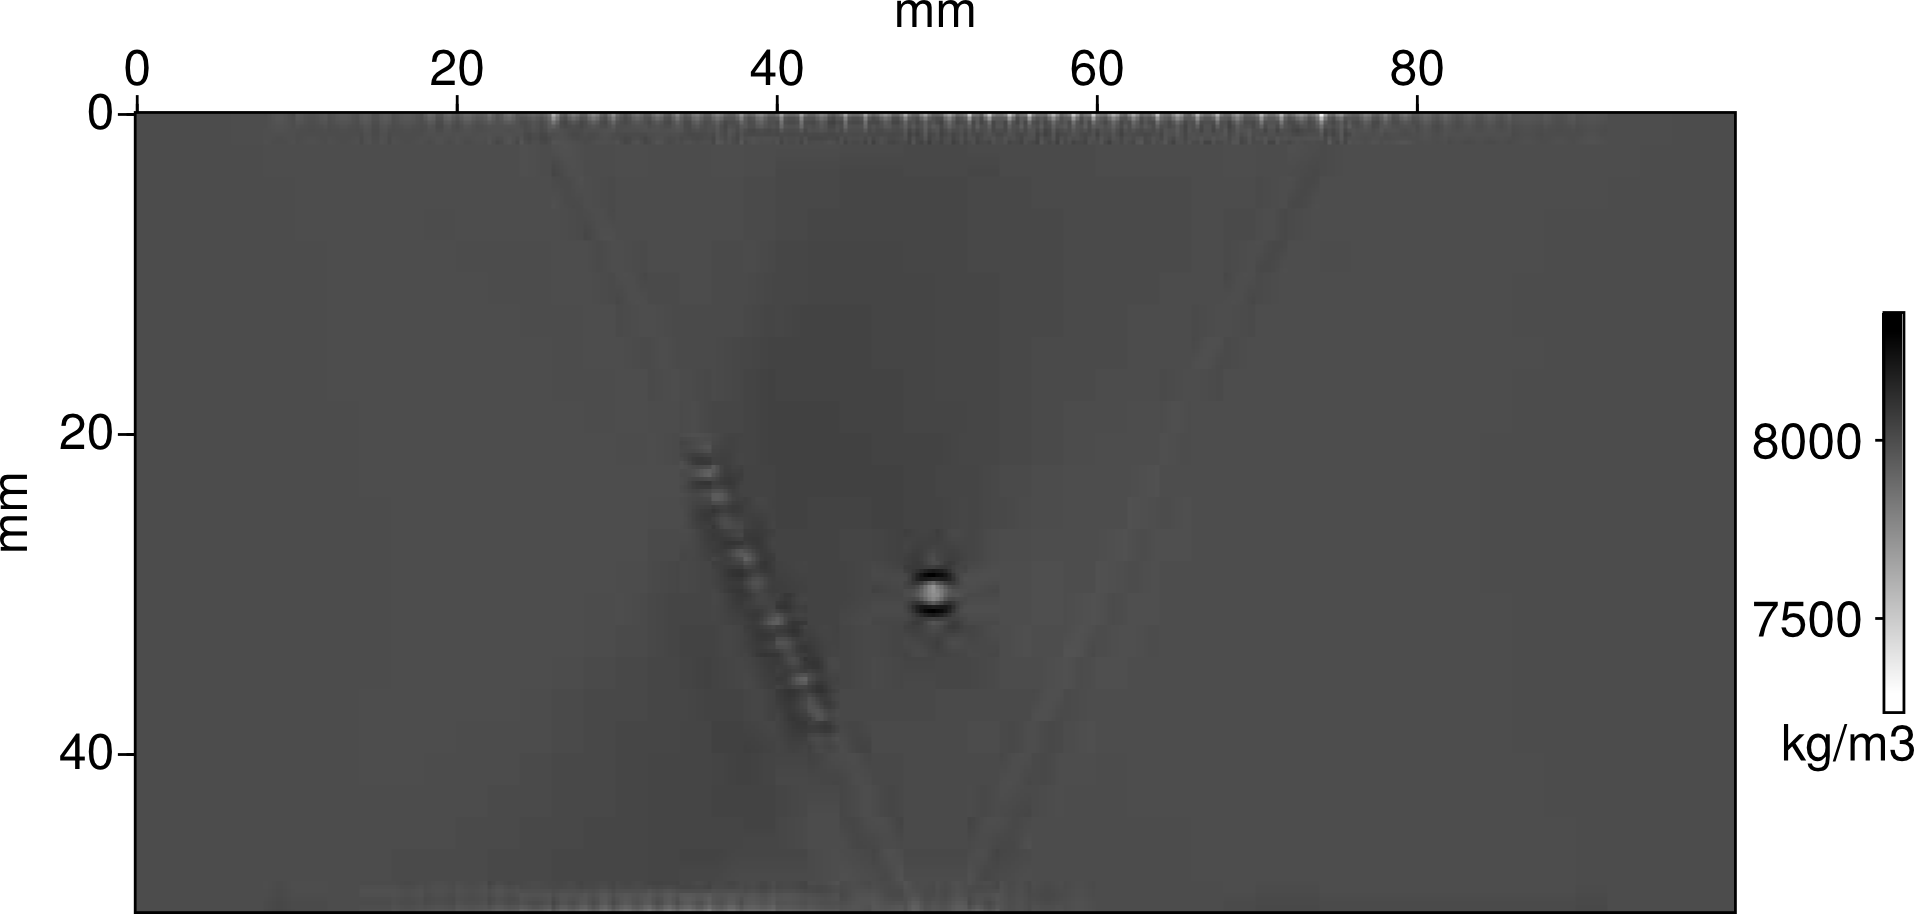
\includegraphics[width=0.7\textwidth]{img/multi/rho_6000k.png}\\	
%		
%		Masse volumique vraie : \\[0.2cm]
%		\includegraphics[width=0.7\textwidth]{img/rho_true.png}
%	\end{columns}	
%	
%\end{small}
%\end{frame}
%
\subsection*{}
\begin{frame}{Isotropic case}
\begin{itemize}
	\item Monoparamter inversion : \\[0.2cm]
	\begin{columns}
		\column{0.5\textwidth}
		\centering
		\small{velocity} \\[0.2cm]
		\includegraphics[width=0.6\textwidth]{img/multi/coupe_vp_mono_smooth_hor.png}\\
		\column{0.5\textwidth}
		\centering
		\small{density} \\[0.2cm]
		\includegraphics[width=0.6\textwidth]{img/multi/coupe_rho_mono.png}\\
	\end{columns}
	\item Multiparameter inversion : \\[0.2cm]
	\begin{columns}
		\column{0.5\textwidth}
		\centering
		\small{velocity} \\[0.2cm]
		\includegraphics[width=0.6\textwidth]{img/multi/coupe_vp_multi.png}\\
		\column{0.5\textwidth}
		\centering
		\small{density} \\[0.2cm]
		\includegraphics[width=0.6\textwidth]{img/multi/coupe_rho_multi.png}\\
	\end{columns}	
\end{itemize}
\centering
\hspace{3cm}Horizontal profiles at 3 cm depth
\end{frame}

\section{HTI case}
\subsection*{}
\begin{frame}{\insertsectionhead}
%\begin{small}
	\begin{columns}
		\centering
		\column{0.5\textwidth}
		\centering
		\begin{itemize}
			\item  Acoustic approximation, transverse isotropic, horizontal symmetry axis\\[0.3cm]
			\item Anisotropy parameters :
		\end{itemize}			 
		\begin{equation*}
			\epsilon = \frac{\bm{v}_{p}.\bm{e}_{x}-\bm{v}_{p}.\bm{e_{z}}}{\bm{v}_{p}.\bm{e}_{z}}
		\end{equation*}
		\column{0.3\textwidth}
		\centering
		\vspace{-0.3cm}\begin{figure}
		\vspace{-0.65cm}\hspace{-0.5cm}\includegraphics[height=4cm]{img/anisotrope/e20.png}\\ \small{Data from true model}
		\end{figure}
		\column{0.3\textwidth}
		\centering
		\vspace{-0.3cm}\begin{figure}
		\vspace{-0.65cm}\hspace{-0.3cm}\includegraphics[height=4cm]{img/anisotrope/residu_init.png}\\ \small{Initial residual data}
		\end{figure}
	\end{columns}	
	\vspace{0.2cm}
	\begin{columns}
		\column{0.5\textwidth}
		\centering
		True $\epsilon$ : \\[0.2cm]
		\includegraphics[width=0.8\textwidth]{img/anisotrope/epsilon_true.png}\\
		
		\column{0.5\textwidth}
		\centering
		Reconstructed $\epsilon$ : \\[0.2cm]
		\includegraphics[width=0.8\textwidth]{img/anisotrope/epsilon_final.png}\\		
	\end{columns}	
%\end{small}
\begin{itemize}
	\item Get info from horizontal rays : $\theta\sim \pi~~~\rightarrow~~k\sim 0$
	\item Not realistic model
\end{itemize}
\end{frame}


\section{Conclusions}
\subsection*{}
\begin{frame}{\insertsectionhead}
\setlength{\leftmargin}{-1cm}
\setlength{\rightmargin}{-1cm}

	\begin{itemize}
		\item<2-> Anisotropy model : 
		\begin{itemize}
			\item acoustic case : tilted transverse isotropic medium
			\item elastic case : $6\times C_{ij}$
		\end{itemize} 
		\begin{figure}[!h]
		    \centering
		    \hspace{-1cm}\begin{subfigure}[b]{0.25\textwidth}
		    	\centering
		 		\includegraphics[height=2cm]{img/ogilvy_model.png}
		 		\vspace{0.2cm}\caption{\centering \scriptsize Grain orientation}
			\end{subfigure}
			\begin{subfigure}[b]{0.7\textwidth}
				\centering
		 		\includegraphics[height=2cm]{img/ogilvy_ray1.png}
		 		\includegraphics[height=2cm]{img/ogilvy_ray2.png}\\
		 		\raggedright{\vspace{-0.25cm}\tiny{\itshape Pictures from~Ogilvy, 1986}}
		 		\caption{\scriptsize Ray tracing (compressional wave) }
			\end{subfigure}\\
				
		\end{figure}	
		\item<3-> Building another initial model 
		\item<4-> Real data application : 3D case
		\item<5-> Real acquisition geometry
			\begin{itemize}
				\item curvature at the top/root of welds
				\item optimial illumination/resolution
			\end{itemize}
	\end{itemize}
	\begin{picture}(0,0)(0,0)\put(240,0){
		\only<4->{
		\begin{tikzpicture}
			\node (a) at (0,0) {\includegraphics[width=2.5cm]{img/linear_array.png}};
			\node (b) [below=-0.2cm of a] {\tiny \itshape Image Olympus};
		\end{tikzpicture}
		}
	}\end{picture}
	
\end{frame}


%\begin{frame}[hide,allowframebreaks]{Références}
%
%	\begin{adjustwidth}{-2em}{-2.5em}
%		\scriptsize
%		\bibliographystyle{abbrvnat}
%		\bibliography{biblio}
%	\end{adjustwidth}
%\end{frame}



\end{document}
